\chapter{Implementasi dan Pengujian}
\label{chap:Implementasi}

Pada bab ini akan ditunjukkan tampilan dari implementasi perangkat lunak dan juga bagaimana perangkat lunak diimplementasikan. Pengujian juga akan diterapkan pada perangkat lunak secara fungsional dan eksperimental. Hasil dari pegujian akan dijelaskan secara rinci dan sistemasi serta akan dibuat kesimpulan untuk pengujian yang telah dilakukan.


% \section{Implementasi Perangkat Lunak}
% \label{sec:implementasi-pl}

% \subsection{Instalasi}
% \label{sec:instalasi}

% \subsection{Antarmuka}
% \label{sec:antarmuka}

% \subsection{Randomisasi}
% \label{sec:randomisasi}


\section{Implementasi Antarmuka}
\label{sec:implementasi-antarmuka}

Antarmuka perangkat lunak diimplementasikan dengan memakai \textit{framework} antarmuka grafis berbasis bahasa pemograman Python yang bernama Kivy\footnote{https://kivy.org/\#home}. Implementasi antarmuka disesuaikan dengan rancangan antarmuka perangkat lunak yang telah dibuat pada bab~\ref{chap:perancangan}. Gambar~\ref{fig:antarmukautama} adalah tampilan antarmuka dari implementasi perangkat lunak.

\begin{figure}
	\centering
	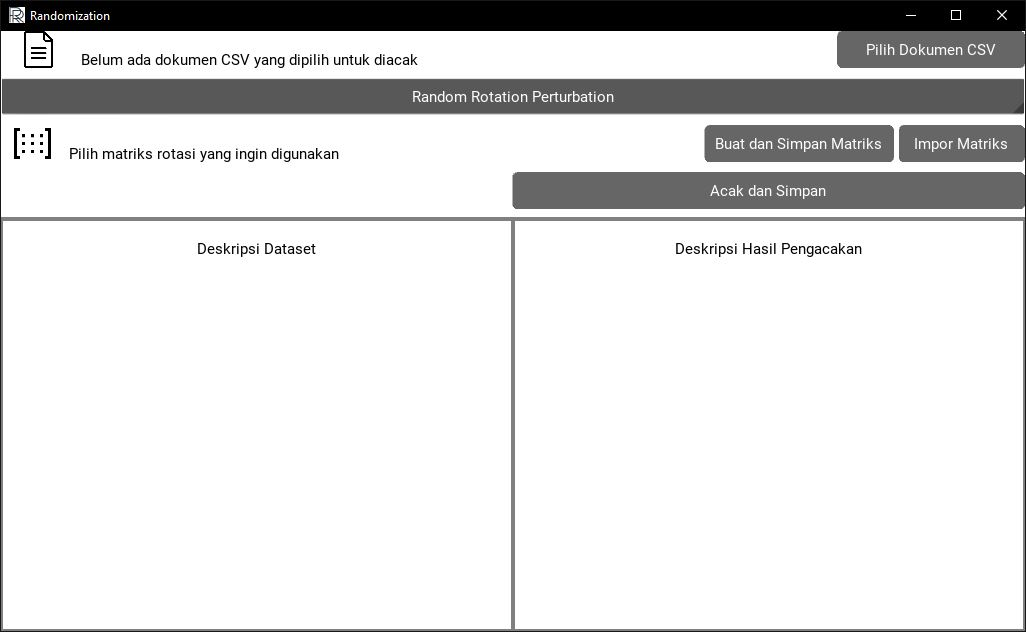
\includegraphics[scale=0.6]{antarmukautama}
	\caption{Tampilan perangkat lunak yang pertama ditampilkan saat perangkat lunak baru dibuka}
	\label{fig:antarmukautama}
\end{figure}

Antarmuka perangkat lunak mempunyai tiga buah bagian yang mempunyai fungsinya masing-masing. Ketiga bagian ini dapat dilihat pada Gambar~\ref{fig:antarmukautamabernomor} Pertama adalah bagian masukan dan pengaturan, terdapat pada bagian atas yang bernomor satu dan dikelilingi kotak merah. Kedua adalah bagian deskripsi dataset, terdapat pada bagian bawah sebelah kiri yang bernomor dua dan dikelilingi kotak biru. Terakhir adalah bagian deskripsi hasil randomisasi, terdapat pada bagian bawah sebelah kanan yang bernomor tiga dan dikelilingi kotak hijau. Ketiga bagian ini akan dijelaskan secara rinci pada subbab-subbab berikutnya.

\begin{figure}
	\centering
	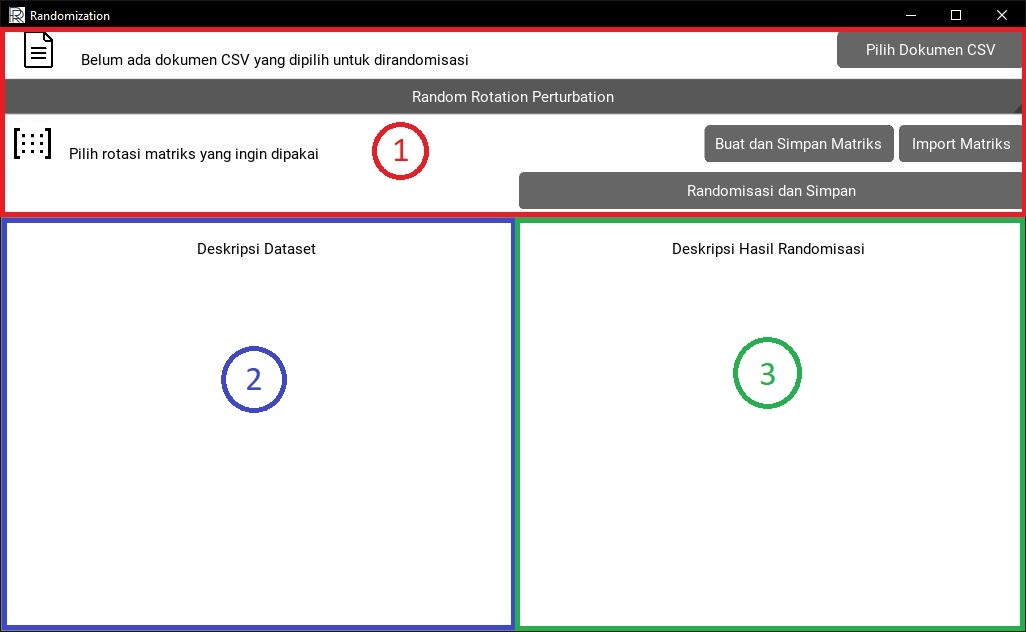
\includegraphics[scale=0.6]{antarmukautamabernomor}
	\caption{Bagian-bagian pada antarmuka perangkat lunak}
	\label{fig:antarmukautamabernomor}
\end{figure}

Perangkat lunak randomisasi ini mengimplementasikan dua buah teknik randomisasi yang berbeda yaitu \textit{Random Rotation Perturbation} dan \textit{Random Projection Perturbation}. Oleh karena itu, antarmuka perangkat lunak akan menyesuaikan dengan teknik yang dipilih oleh pengguna. Ketiga bagian antarmuka yang telah disebutkan tadi dengan otomatis akan berubah sesuai dengan teknik yang dipilih. Pada setiap subbab akan dijelaskan juga sekaligus perbedaan antarmuka teknik randomisasi satu dengan yang lainnya.

\subsection{Masukan dan Pengaturan}
\label{sec:masukanpengaturan}

Bagian masukan dan pengaturan menyediakan berbagai interaksi untuk pengguna dapat mengatur masukan yang perlu diberikan kepada perangkat lunak dan menerapkan teknik randomisasi yang diinginkan. Ada beberapa fungsi inti pada bagian ini yaitu masukan dataset berupa file \textit{comma-separated values} yang ingin dirandomisasi, memilih teknik randomisasi yang ingin digunakan, membuat baru dan memilih matriks rotasi atau proyeksi yang ingin digunakan, masukan nilai variabel Epsilon dan nilai variabel K untuk teknik \textit{Random Projection Perturbation}, dan sebuah tombol untuk menerapkan teknik randomisasi dan menyimpan hasilnya. Berikut akan dijelaskan secara rinci dengan gambar setiap fungsi tersebut yang dapat dilihat pada Gambar~\ref{fig:antarmukamasukanpengaturan} dan cara pemakaiannya yang benar secara berturut. 

\begin{figure}
	\centering
	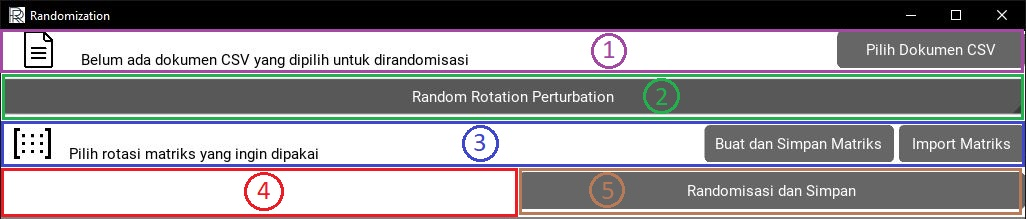
\includegraphics[scale=0.6]{antarmukamasukanpengaturan}
	\caption{Bagian antarmuka masukan dan pengaturan perangkat lunak}
	\label{fig:antarmukamasukanpengaturan}
\end{figure}

\subsubsection{Masukan Dataset}
\label{sec:masukandataset}

Pertama pengguna perlu memberikan masukan dataset yang ingin dirandomisasi berupa dokumen berjenis \textit{comma-separated values}. Perangkat lunak menyediakan fitur tersebut yang dapat dilihat pada Gambar~\ref{fig:antarmukamasukanpengaturan} yang terdapat pada bagian yang dikelilingi kotak berwarna merah dan bernomor satu. Pengguna dapat menekan tombol \textquotedblleft Pilih Dokumen CSV\textquotedblright~yang terletak pada ujung sebelah kanan. Tombol ini bertujuan untuk memilih dokumen yang ingin dirandomisasi pada direktori pengguna. Ketika tombol ditekan, perangkat lunak akan membuka jendela baru untuk memilih dokumen yang dapat dilihat pada gambar~\ref{fig:pilihdokumen}.

\begin{figure}
	\centering
	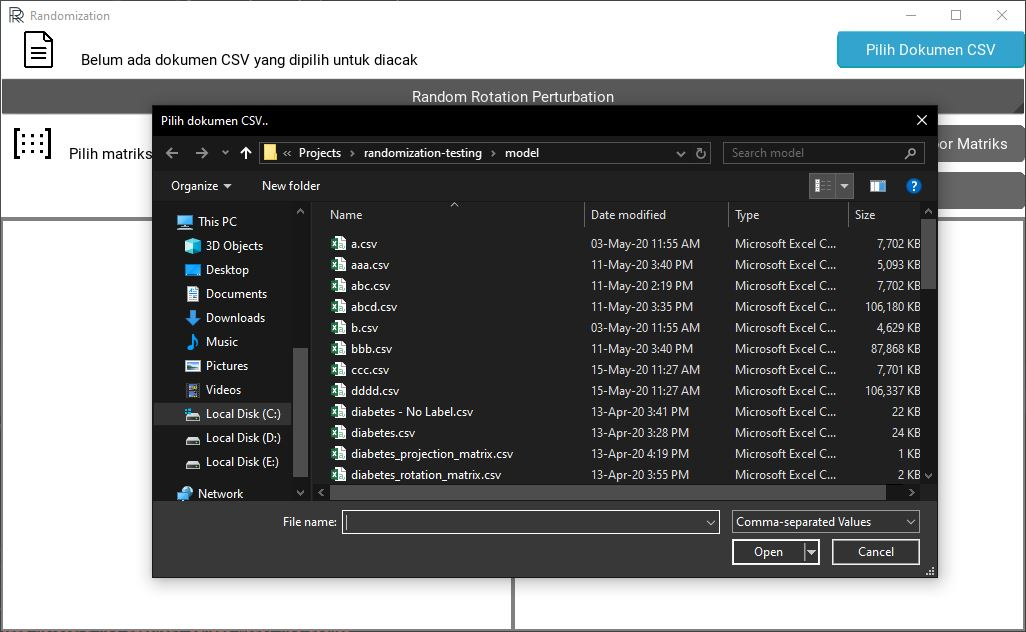
\includegraphics[scale=0.6]{pilihdokumen}
	\caption{Jendela untuk memilih dataset yang berupa dokumen CSV}
	\label{fig:pilihdokumen}
\end{figure}

Setelah pengguna memilih dataset yang diinginkan, perangkat lunak akan otomatis menuliskan lokasi dokumen yang dipilih berada. Perangkat lunak akan menampilkan lokasi dokumen tersebut pada bagian tengah sebelah kanan simbol dokumen dan sebelah kiri tombol \textquotedblleft Pilih Dokumen CSV\textquotedblright. Jika belum ada dataset yang dipilih maka perangkat lunak akan menampilkan label yang berupa kalimat \textquotedblleft Belum ada dokumen CSV yang dipilih untuk dirandomisasi\textquotedblright~yang menunjukkan bahwa belum ada dokumen yang dipilih oleh pengguna. Jika pengguna memilih ulang dokumen, maka secara otomatis juga perangkat lunak akan memperbaharui lokasi dokumen sesuai dokumen yang dipilih pengguna.

Apabila dokumen yang dipilih berukuran besar, maka perangkat lunak akan memakan sedikit waktu yang lebih lama. Dalam rangka memberitahukan kepada pengguna bahwa perangkat lunak sedang melakukan proses pemilihan dokumen, perangkat lunak akan menampilkan sebuah \textit{popup} yang memberitahukan bahwa proses pemilihan sedang berjalan dan perangkat lunak tidak berhenti bekerja maupun \textit{error} sehingga pengguna tidak bingung apabila perangkat lunak memakan waktu yang lebih lama untuk memproses dokumen yang dipilih. Tampilan antarmuka \textit{popup} tersebut dapat dilihat pada Gambar~\ref{fig:loadingmemilihdokumen}. Setelah dokumen dipilih pengguna dan perangkat lunak berhasil memproses dokumen tersebut, perangkat lunak akan memperbaharui lokasi dokumen dan menampilkan beberapa informasi dataset yang dipilih pada bagian deskripsi dataset yang akan dijelaskan pada subbab berikutnya. Tampilan antarmuka setelah pengguna memilih dokumen dapat dilihat pada Gambar~\ref{fig:dokumendipilih}

\begin{figure}
	\centering
	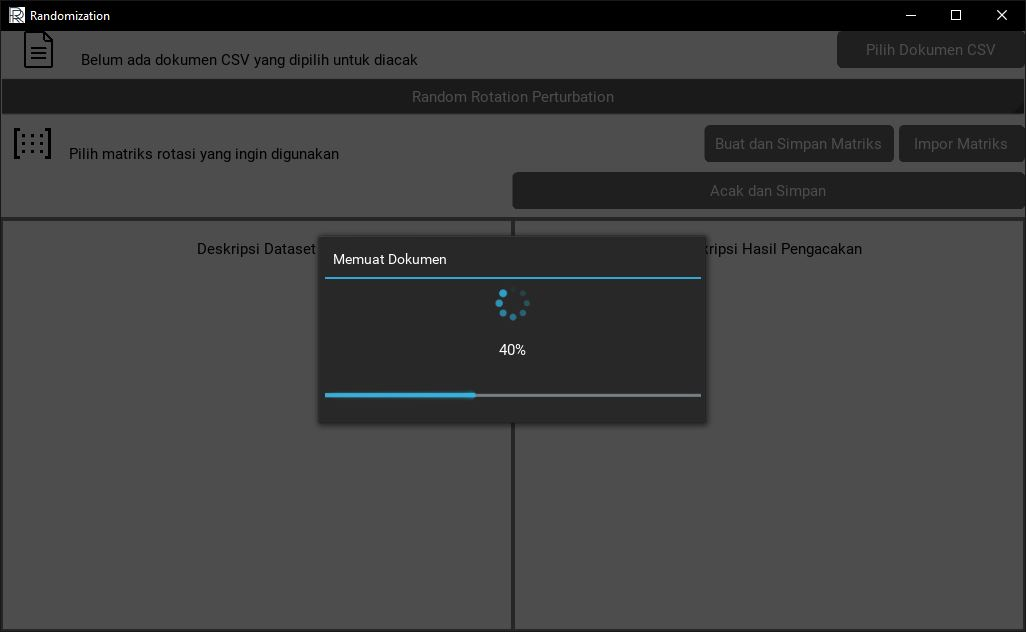
\includegraphics[scale=0.6]{loadingmemilihdokumen}
	\caption{Tampilan \textit{popup} yang ditampilkan saat proses berlangsung}
	\label{fig:loadingmemilihdokumen}
\end{figure}

\begin{figure}
	\centering
	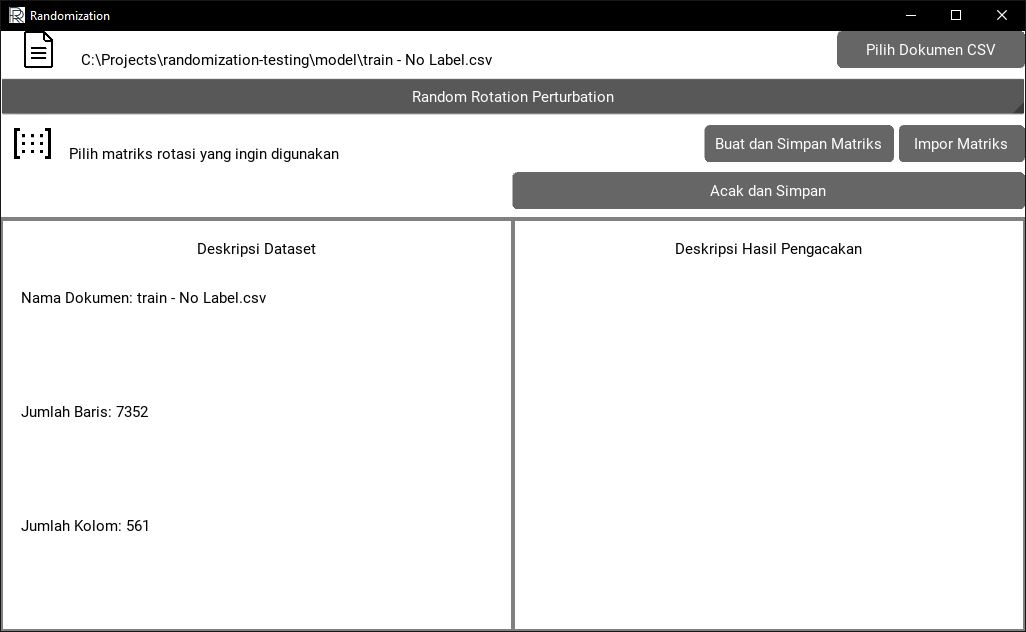
\includegraphics[scale=0.6]{dokumendipilih}
	\caption{Tampilan antarmuka setelah sebuah dokumen dipilih}
	\label{fig:dokumendipilih}
\end{figure}

Selain itu setelah pengguna memilih dokumen CSV, perangkat lunak akan membaca dokumen tersebut dan memproses isi dari dokumen tersebut menjadi dataset yang berupa matriks. Proses ini dilakukan sekali saja tepat setelah pengguna memilih dokumen dengan menekan tombol \textquotedblleft Pilih Dokumen CSV\textquotedblright. Oleh karena itu, apabila sebuah dokumen CSV diubah isinya setelah dokumen tersebut dipilih oleh pengguna maka perangkat lunak tetap akan menggunakan isi dari dokumen tersebut yang belum diubah. Pengguna harus berhati-hati apabila isi dokumen diubah maka pengguna juga harus memilih kembali dokumen yang sama tersebut walaupun perangkat lunak sudah menunjukkan lokasi dokumen yang digunakan adalah dokumen yang pengguna inginkan.

\subsubsection{Pemilihan Teknik Randomisasi}
\label{sec:pilihteknik}

Setelah pengguna memilih dataset yang ingin dirandomisasi, pengguna juga harus memilih teknik randomisasi apa yang ingin diterapkan terhadap dataset yang sudah dipilih. Pada awal perangkat lunak dibuka, secara otomatis teknik \textit{Random Rotation Perturbation} yang dipilih. Apabila pengguna ingin mengganti teknik yang ingin diterapkan pada dataset, pengguna dapat menekan tombol \textit{dropdown} yang bertuliskan nama teknik randomisasi. Tombol ini dapat dilihat pada Gambar~\ref{fig:antarmukamasukanpengaturan} yang dikelilingi kotak berwarna hijau dan bernomor dua.

Apabila pengguna menekan tombol ini maka perangkat lunak akan menampilkan \textit{dropdown} yang mempunyai dua buah opsi teknik randomisasi yaitu \textquotedblleft Random Rotation Perturbation\textquotedblright~dan \textquotedblleft Random Projection Perturbation\textquotedblright. Antarmuka tersebut dapat dilihat pada Gambar~\ref{fig:opsipilihteknik} yang dikelilingi oleh kotak merah. Pemilihan teknik ini juga akan memicu beberapa perubahan pada tampilan antarmuka perangkat lunak menyesuaikan dengan teknik yang dipilih. Beberapa perubahan pada perangkat lunak tersebut melingkupi bagian pembuatan dan pemilihan matriks, parameter teknik randomisasi, dan bagian randomisasi dan simpan yang akan dijelaskan setiap perubahan tersebut pada subbab berikutnya.

\begin{figure}
	\centering
	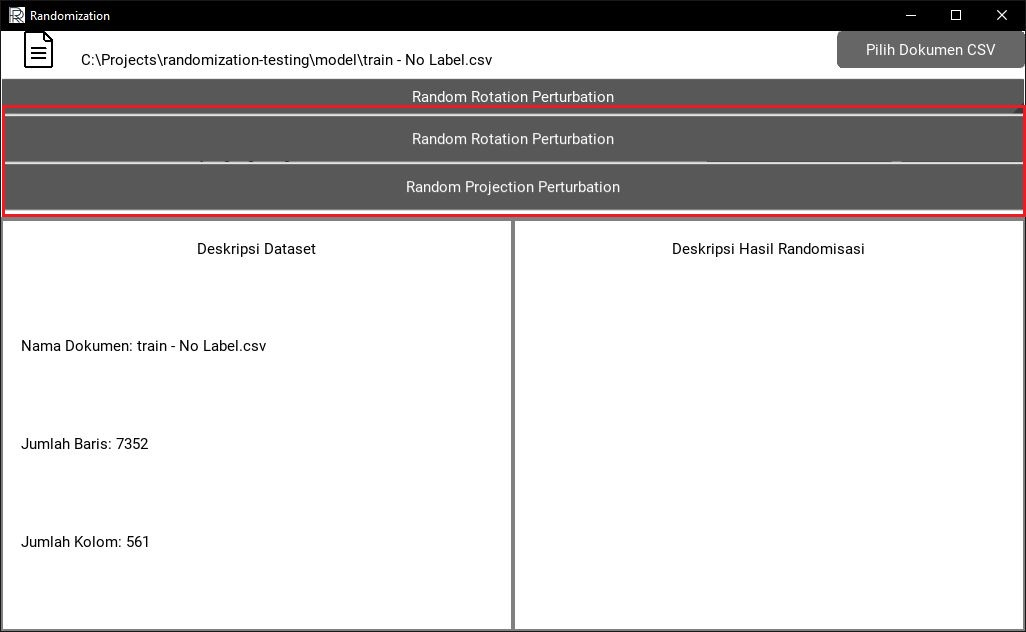
\includegraphics[scale=0.6]{opsipilihteknik}
	\caption{Tampilan antarmuka saat pengguna memilih teknik}
	\label{fig:opsipilihteknik}
\end{figure}

\subsubsection{Pembuatan dan Pemilihan Matriks}
\label{sec:pilihmatriks}

Setelah pengguna memilih teknik yang ingin diterapkan, pengguna harus memilih matriks yang diinginkan atau membuat baru. Matriks yang dimaksudkan adalah matriks rotasi atau matriks proyeksi sesuai teknik randomisasi yang dipilih. Apabila teknik \textit{Random Rotation Perturbation} yang dipilih maka perangkat lunak akan mengubah fungsi pembuatan dan pemilihan matriks ini menjadi matriks rotasi. Apabila teknik \textit{Random Projection Perturbation} yang dipilih maka perangkat lunak akan mengubah fungsi pembuatan dan pemilihan matriks ini menjadi matriks proyeksi. Perubahan ini dapat terlihat pada label yang berada di sebelah kanan simbol matriks apabila belum memilih atau membuat matriks maka label tersebut akan menampilkan kalimat \textquotedblleft Pilih matriks rotasi yang ingin digunakan\textquotedblright~atau \textquotedblleft Pilih matriks proyeksi yang ingin digunakan\textquotedblright. Bagian ini dapat dilihat pada Gambar~\ref{fig:antarmukamasukanpengaturan} yang dikelilingi oleh kotak berwarna hijau dan bernomor dua.

Ada dua buah tombol pada bagian ini yaitu \textquotedblleft Buat dan Simpan Matriks\textquotedblright~dan \textquotedblleft Import Matriks\textquotedblright. Tombol \textquotedblleft Buat dan Simpan Matriks\textquotedblright~mempunyai fungsi untuk membuat matriks rotasi atau proyeksi baru sesuai teknik randomisasi yang dipilih dan menyimpan matriks tersebut pada sebuah dokumen CSV baru yang dibuat oleh perangkat lunak pada direktori tertentu yang akan dipilih oleh pengguna. Pada saat perangkat lunak sedang memproses matriks tersebut, perangkat lunak akan menampilkan \textit{popup} memuat yang dapat dilihat pada Gambar~\ref{fig:buatsimpanmatriks}. \textit{Popup} ini juga akan tampil saat proses impor matriks dilakukan. Hasil matriks yang dibuat oleh perangkat lunak dapat digunakan kembali untuk lain kali sehingga rotasi atau proyeksi yang diterapkan akan sama dengan yang sebelumnya. 

Pengguna dapat melakukan impor matriks dengan cara menekan tombol \textquotedblleft Import Matriks\textquotedblright~untuk memilih matriks rotasi atau proyeksi yang diinginkan untuk diterapkan pada dataset. Matriks yang dipilih harus sesuai dengan dataset yang ingin dirandomisasi, misalnya apabila matriks rotasi yang dipilih memiliki dimensi yang berbeda dengan dataset maka perangkat lunak akan melarang impor matriks dilakukan karena randomisasi tidak dapat dilakukan. Perangkat lunak akan menampilkan \textit{popup} peringatan untuk pengguna yang dapat dilihat pada Gambar~\ref{fig:matrikstidaksesuai}. Apabila pengguna memilih teknik \textit{Random Projection Perturbation} dan pengguna mengimpor matriks proyeksi maka parameter variabel K akan terisi secara otomatis sesuai dengan matriks proyeksi yang diimpor.

\begin{figure}
	\centering
	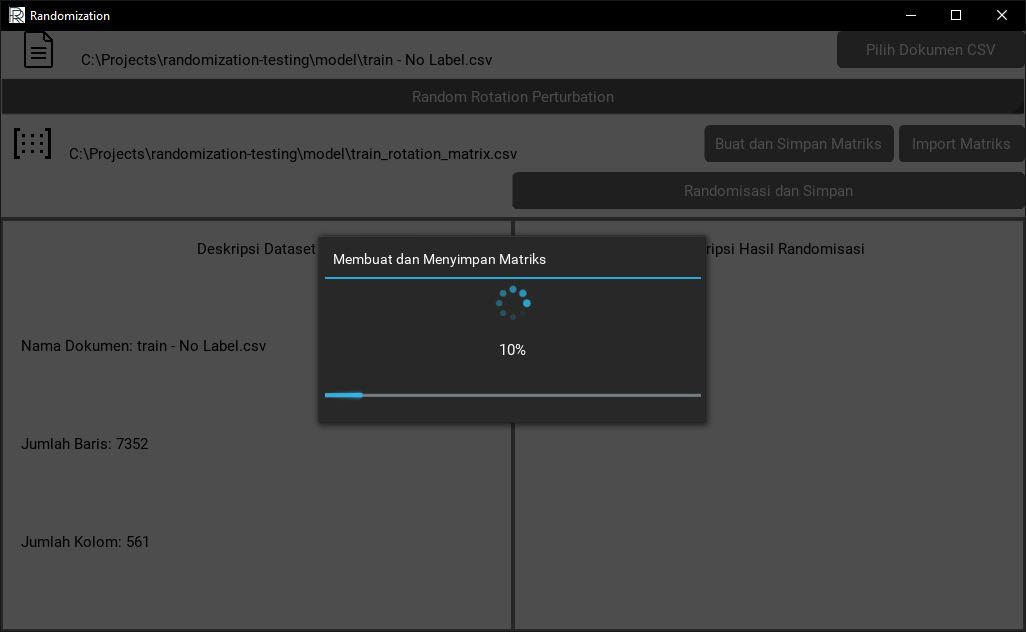
\includegraphics[scale=0.6]{buatsimpanmatriks}
	\caption{Tampilan antarmuka saat perangkat lunak membuat dan menyimpan matriks}
	\label{fig:buatsimpanmatriks}
\end{figure}

\begin{figure}
	\centering
	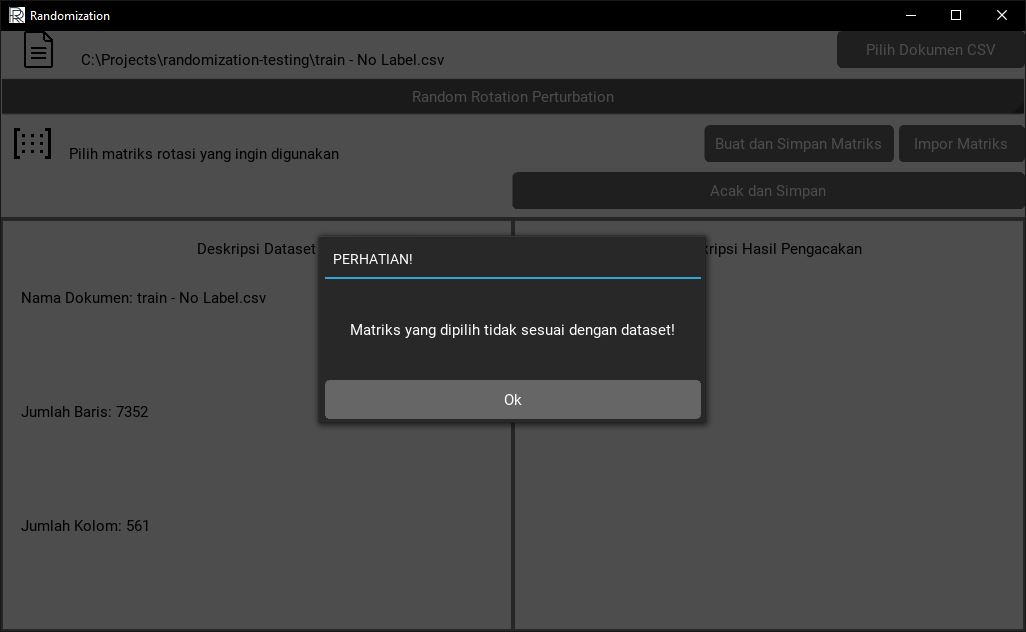
\includegraphics[scale=0.6]{matrikstidaksesuai}
	\caption{Tampilan \textit{popup} yang ditampilkan apabila matriks yang ingin diimpor tidak sesuai dengan dataset}
	\label{fig:matrikstidaksesuai}
\end{figure}

Apabila pengguna belum memilih dataset yang ingin dirandomisasi, pengguna tidak dapat membuat maupun impor matriks terlebih dahulu. Hal ini dikarenakan perlu ada proses pengecekan terlebih dahulu yang dilakukan perangkat lunak untuk memastikan dataset yang ingin dirandomisasi sudah sesuai persyaratan dan sesuai dengan matriks yang akan dipilih. Perangkat lunak akan melarang pengguna membuat maupun impor matriks dengan menampilkan sebuah \textit{popup} peringatan yang dapat dilihat pada Gambar~\ref{fig:larangmatriks}. Pada teknik \textit{Random Projection Perturbation}, pengguna baru bisa membuat matriks proyeksi apabila sudah memenuhi persyaratan yang diminta yaitu mengisi parameter teknik tersebut yang mana adalah variabel Epsilon dan variabel K.

\begin{figure}
	\centering
	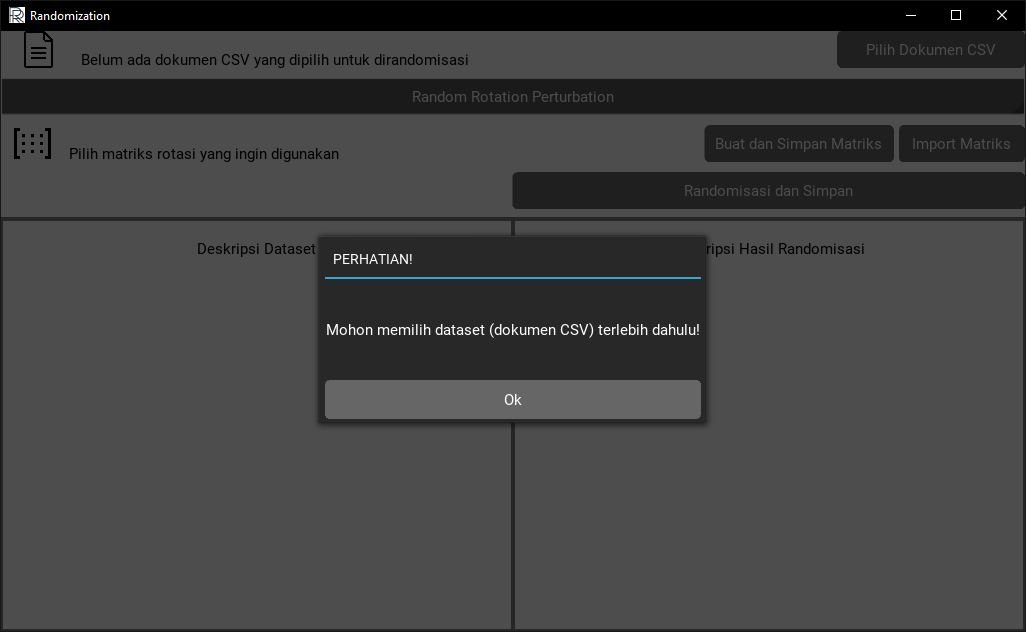
\includegraphics[scale=0.6]{larangmatriks}
	\caption{Tampilan \textit{popup} yang ditampilkan apabila pengguna belum memilih dataset yang ingin dirandomisasi}
	\label{fig:larangmatriks}
\end{figure}

\subsubsection{Parameter Teknik Randomisasi}
\label{sec:parameterteknik}

Perangkat lunak hanya meminta kepada pengguna parameter untuk teknik \textit{Random Projection Perturbation} saja apabila pengguna memilih teknik tersebut. Pada teknik \textit{Random Rotation Perturbation} tidak ada parameter yang perlu pengguna berikan. Ada dua buah parameter yang perlu pengguna berikan yaitu variabel Epsilon dan variabel K. Pengguna dapat memasukkan nilai kedua variabel tersebut dengan menekan kolom variabel tersebut masing-masing. Kedua buah parameter tersebut dapat dilihat antarmukanya pada Gambar~\ref{fig:parameterprojection}

\begin{figure}
	\centering
	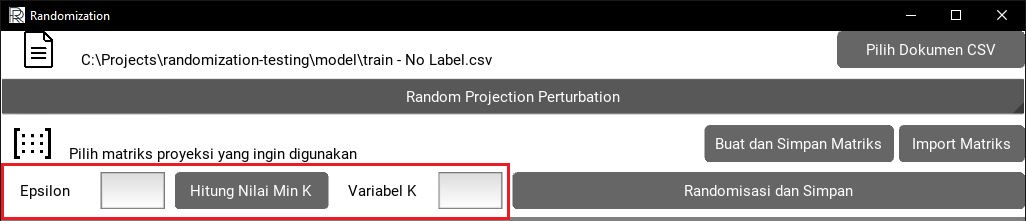
\includegraphics[scale=0.6]{parameterprojection}
	\caption{Tampilan antarmuka parameter teknik randomisasi \textit{Random Projection Perturbation}}
	\label{fig:parameterprojection}
\end{figure}

Seperti yang disinggung pada subbab sebelumnya antarmuka perangkat lunak akan menyesuaikan secara otomatis sesuai teknik yang dipilih pengguna. Pada bagian parameter teknik randomisasi, perangkat lunak akan menyembunyikan antarmuka parameter \textit{Random Projection Perturbation} apabila pengguna memilih teknik \textit{Random Rotation Perturbation}. Antarmuka tersebut dapat dilihat pada Gambar~\ref{fig:antarmukamasukanpengaturan} yang dikelilingi oleh kotak berwarna merah dan bernomor empat, dapat dilihat tidak ada parameter apapun yang tampil apabila teknik \textit{Random Rotation Perturbation} yang dipilih.

Selain dua buah parameter, pada bagian ini juga ada sebuah tombol yaitu \textquotedblleft Hitung Nilai Min K\textquotedblright~yang memiliki fungsi untuk menghitung nilai minimal variabel K yang pengguna berikan. Pada teknik \textit{Random Projection Perturbation}, ada beberapa persyaratan yang harus dipenuhi oleh pengguna dan salah satunya adalah variabel K yang diberikan harus melebihi sebuah nilai minimal yang dihitung berdasarkan ukuran dataset dan nilai variabel Epsilon. Oleh karena itu, sebelum tombol ini dapat berfungsi, pengguna harus memilih terlebih dahulu dataset yang ingin dirandomisasi dan memberikan masukan nilai variabel Epsilon yang sesuai dengan persyaratan variabel Epsilon yaitu nilainya lebih besar dari 0 dan kurang dari 1. Apabila pengguna belum memenuhi kedua persyaratan tersebut, tombol tidak akan berfungsi dan perangkat lunak akan menampilkan \textit{popup} peringatan yang dapat dilihat pada Gambar~\ref{fig:popuphitungk}. Nilai minimal variabel K akan ditampilkan pada bagian antarmuka deskripsi dataset yang akan dijelaskan pada subbab berikutnya.

\begin{figure}
	\centering
	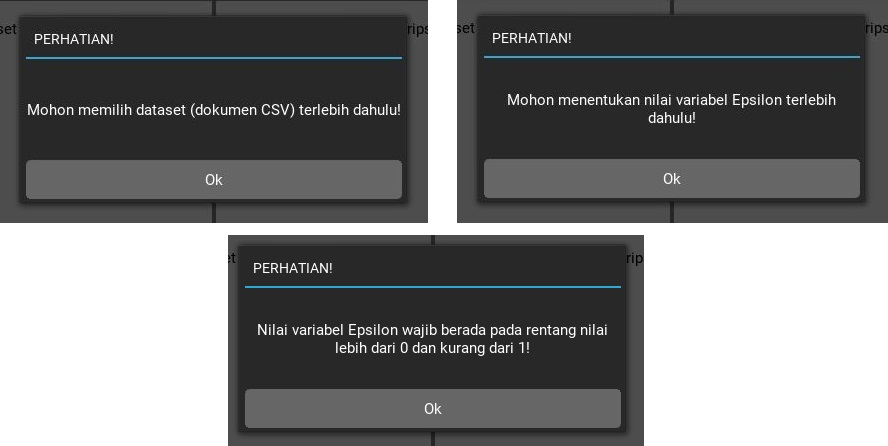
\includegraphics[scale=0.6]{popuphitungk}
	\caption{Tampilan \textit{popup} peringatan tombol \textquotedblleft Hitung Nilai Min K\textquotedblleft }
	\label{fig:popuphitungk}
\end{figure}

Perangkat lunak juga akan memberikan peringatan apabila nilai minimal K melebihi dimensi dari dataset yang ingin dirandomisasi karena salah satu persyaratan dari teknik \textit{Random Projection Perturbation} adalah nilai variabel K harus lebih kecil daripada jumlah dimensi pada dataset yang ingin dirandomisasi. Apabila pengguna melakukan impor matriks maka variabel K akan terisi secara otomatis dan pengguna harus menyesuaikan nilai variabel Epsilon dengan variabel K yang tidak boleh diubah oleh pengguna. 

\subsubsection{Randomisasi dan Simpan}
\label{sec:randomisasisimpan}

Setelah pengguna memberikan masukan yang sesuai dan mengatur pengaturan yang diinginkan maka pengguna telah dapat melakukan randomisasi dengan menekan tombol \textquotedblleft Randomisasi dan Simpan\textquotedblright. Tombol ini akan menerapkan teknik randomisasi yang dipilih oleh pengguna terhadap dataset yang ingin dirandomisasi menggunakan matriks yang telah dibuat atau dipilih oleh pengguna dan parameter-parameter yang pengguna berikan. Tampilan antarmuka saat proses randomisasi dilakukan perangkat lunak dapat dilihat pada Gambar~\ref{fig:loadingrandomisasi}.

\begin{figure}
	\centering
	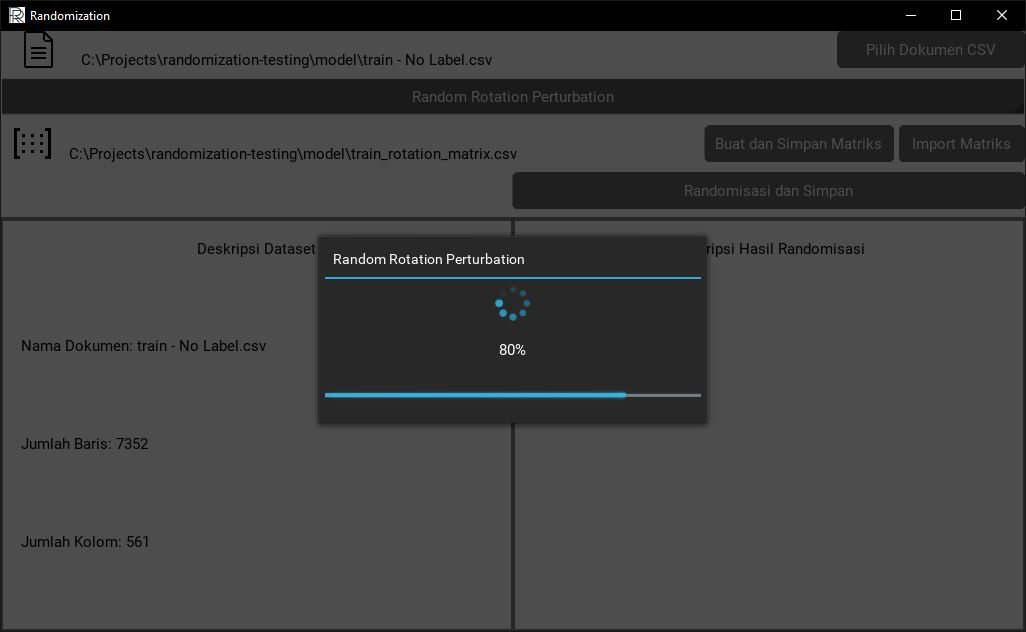
\includegraphics[scale=0.6]{loadingrandomisasi}
	\caption{Tampilan saat perangkat lunak sedang melakukan proses randomisasi}
	\label{fig:loadingrandomisasi}
\end{figure}

Setelah perangkat lunak berhasil melakukan randomisasi, perangkat lunak akan meminta pengguna untuk memilih direktori tempat penyimpanan dan nama dokumen hasil randomisasi. Perangkat lunak akan menyimpan hasil randomisasi dalam bentuk dokumen berjenis \textit{comma-separated values}. Jendela baru untuk memilih direktori penyimpanan akan ditampilkan perangkat lunak, apabila pengguna membatalkan atau dengan kata lain menutup jendela tersebut tanpa memilih direktori penyimpanan maka perangkat lunak tidak akan melanjutkan proses randomisasi dan dianggap gagal. Tampilan antarmuka \textit{popup} yang akan tampil setelah perangkat lunak berhasil melakukan proses randomisasi dan menyimpan hasilnya pada direktori yang pengguna pilih dapat dilihat pada Gambar~\ref{fig:popupberhasilrandomisasi}. Perangkat lunak juga akan menampilkan berbagai informasi hasil randomisasi pada bagian antarmuka deskripsi hasil randomisasi yang akan dijelaskan pada subbab berikutnya.

\begin{figure}
	\centering
	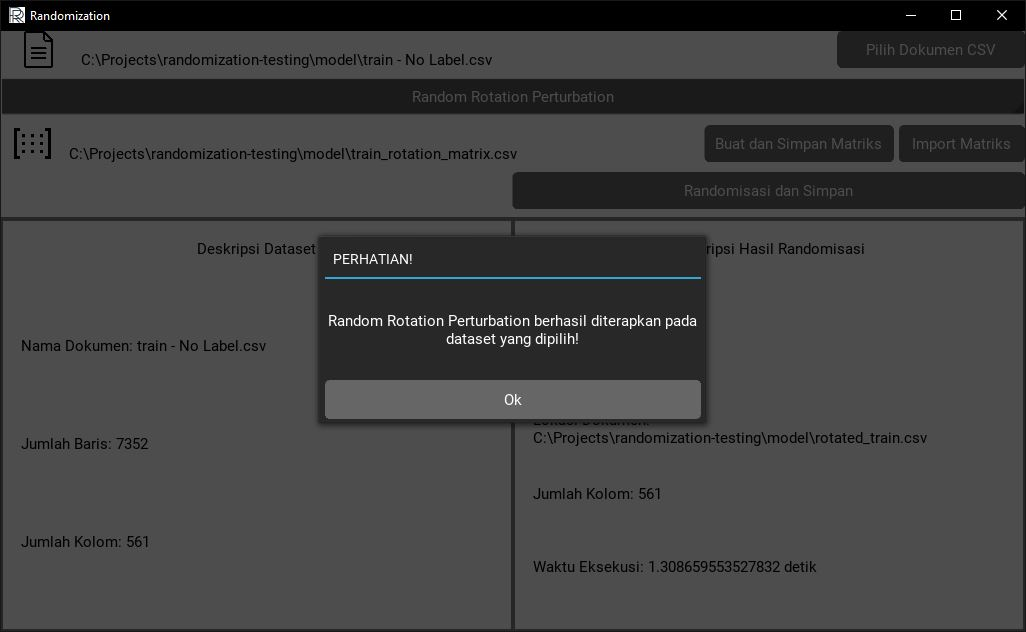
\includegraphics[scale=0.6]{popupberhasilrandomisasi}
	\caption{Tampilan \textit{popup} untuk memberitahukan pengguna bahwa randomisasi berhasil dilakukan}
	\label{fig:popupberhasilrandomisasi}
\end{figure}

Ada beberapa persyaratan yang harus dipenuhi oleh pengguna sebelum melakukan randomisasi yaitu memilih dataset yang ingin dirandomisasi, memilih teknik randomisasi yang diinginkan, membuat atau memilih matriks rotasi atau proyeksi, dan memberikan masukan nilai yang sesuai persyaratan yang ada kepada parameter-parameter teknik randomisasi. Apabila ada persyaratan yang tidak dipenuhi oleh pengguna maka perangkat lunak akan menampilkan \textit{popup} untuk memberikan peringatan kepada pengguna dan perangkat lunak tidak akan melanjutkan proses randomisasi. Perangkat lunak akan menampilkan \textit{popup} peringatan terhadap pelanggaran masing-masing persyaratan tersebut, salah satu contoh tampilan antarmuka \textit{popup} tersebut dapat dilihat pada Gambar~\ref{fig:popupdataset}.

\begin{figure}
	\centering
	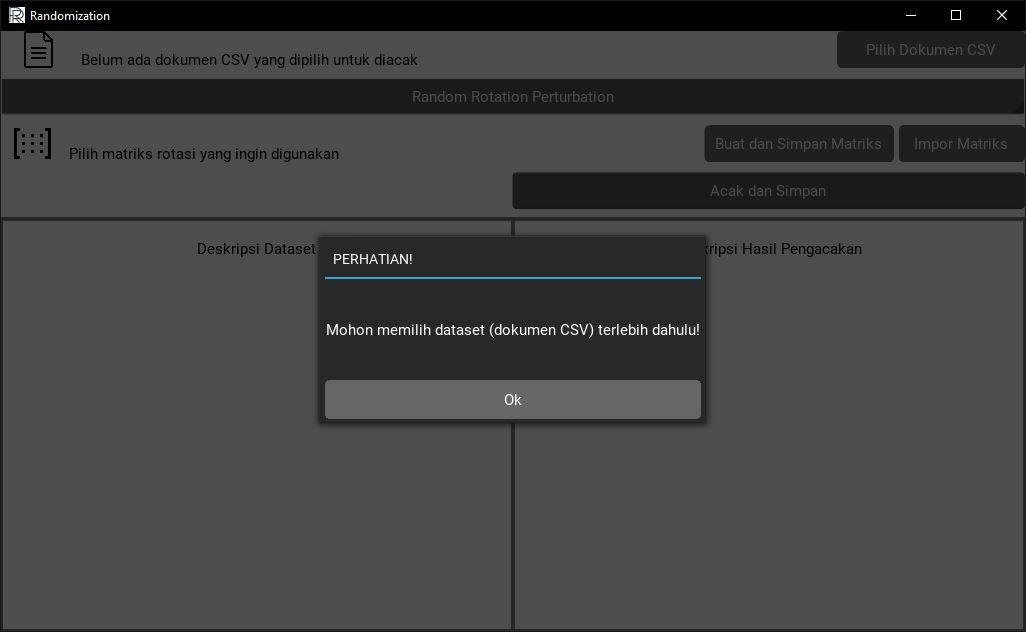
\includegraphics[scale=0.6]{popupdataset}
	\caption{Tampilan \textit{popup} peringatan apabila pengguna belum memilih dataset yang diinginkan untuk dirandomisasi}
	\label{fig:popupdataset}
\end{figure}

\subsection{Deskripsi Dataset}
\label{sec:deskripsidataset}

Pengguna dapat melihat berbagai informasi dokumen \textit{comma-separated values} yang dipilih sebagai dataset yang ingin dirandomisasi pada bagian antarmuka deskripsi dataset. Perangkat lunak akan menampilkan berbagai informasi dataset yaitu nama dokumen, jumlah baris dataset, jumlah kolom dataset, dan nilai minimal variabel K. Seperti yang disinggung pada subbab sebelumnya, pada awalnya nilai minimal variabel K belum diketahui karena belum dihitung. Pengguna harus mengisi variabel Epsilon dan menekan tombol \textquotedblleft Hitung Nilai Min K\textquotedblright~agar perangkat lunak menghitung nilai minimal variabel K dan dapat menampilkannya pada deskripsi dataset.

Bagian antarmuka deskripsi dataset ini akan selalu secara otomatis diperbaharui setiap pengguna memilih dataset baru. Tampilan antarmuka bagian deskripsi dataset dapat dilihat pada Gambar~\ref{fig:antarmukautamabernomor} yang dikelilingi oleh kotak berwarna biru dan bernomor dua. Apabila pengguna telah memilih dataset yang diinginkan untuk dirandomisasi maka perangkat lunak secara otomatis akan memperbaharui tampilan antarmuka deskripsi dataset yang dapat dilihat pada Gambar~\ref{fig:antarmukadeskripsidataset}

\begin{figure}
	\centering
	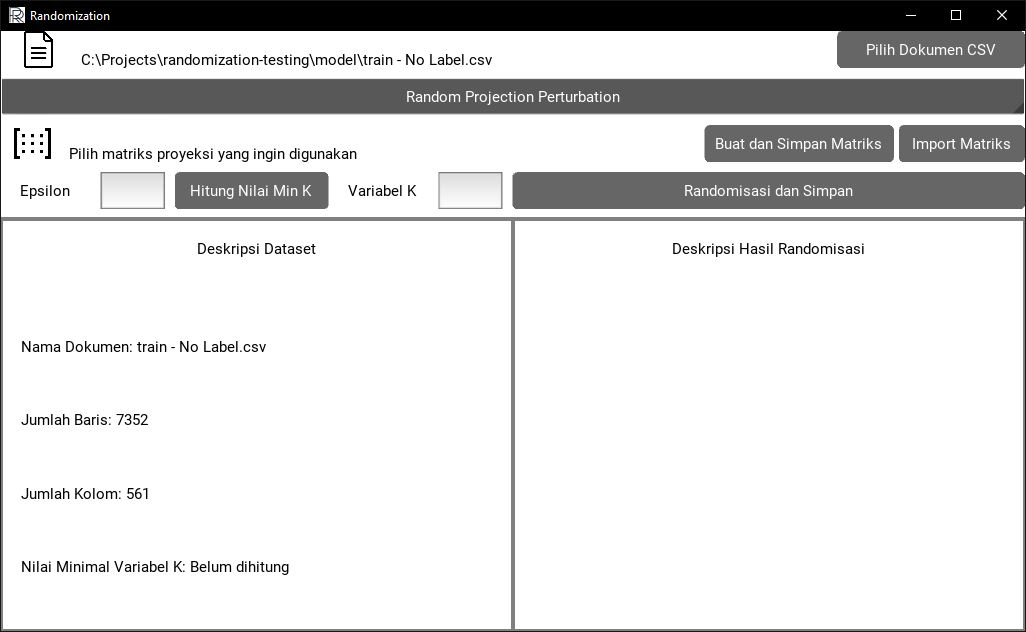
\includegraphics[scale=0.6]{antarmukadeskripsidataset}
	\caption{Tampilan antarmuka deskripsi dataset setelah pengguna memilih dataset yang ingin dirandomisasi}
	\label{fig:antarmukadeskripsidataset}
\end{figure}

\subsection{Deskripsi Hasil Randomisasi}
\label{sec:masukanpengaturan}

Perangkat lunak akan menampilkan isi dari deskripsi hasil randomisasi setelah pengguna menekan tombol \textquotedblleft Randomisasi dan Simpan\textquotedblright~dan perangkat lunak melakukan proses randomisasi. Bagian deskripsi hasil randomisasi ini akan menampilkan informasi-informasi yang berkaitan dengan hasil randomisasi dan deskripsi dataset yang baru. Informasi-informasi tersebut adalah status, lokasi dokumen, lokasi dokumen matriks yang dipakai, jumlah kolom, waktu eksekusi, nilai variabel Epsilon yang digunakan, dan nilai variabel K yang digunakan. Dua informasi terakhir tersebut hanya tampil apabila pengguna memilih teknik randomisasi \textquotedblleft Random Projection Perturbation\textquotedblright.

Bagian antarmuka deskripsi dataset ini akan selalu secara otomatis diperbaharui setiap pengguna memilih dataset baru. Tampilan antarmuka bagian deskripsi dataset dapat dilihat pada Gambar~\ref{fig:antarmukautamabernomor} yang dikelilingi oleh kotak berwarna biru dan bernomor dua. Apabila pengguna telah memilih dataset yang diinginkan untuk dirandomisasi maka perangkat lunak secara otomatis akan memperbaharui tampilan antarmuka deskripsi dataset yang dapat dilihat pada Gambar~\ref{fig:antarmukahasilrandomisasi}

\begin{figure}
	\centering
	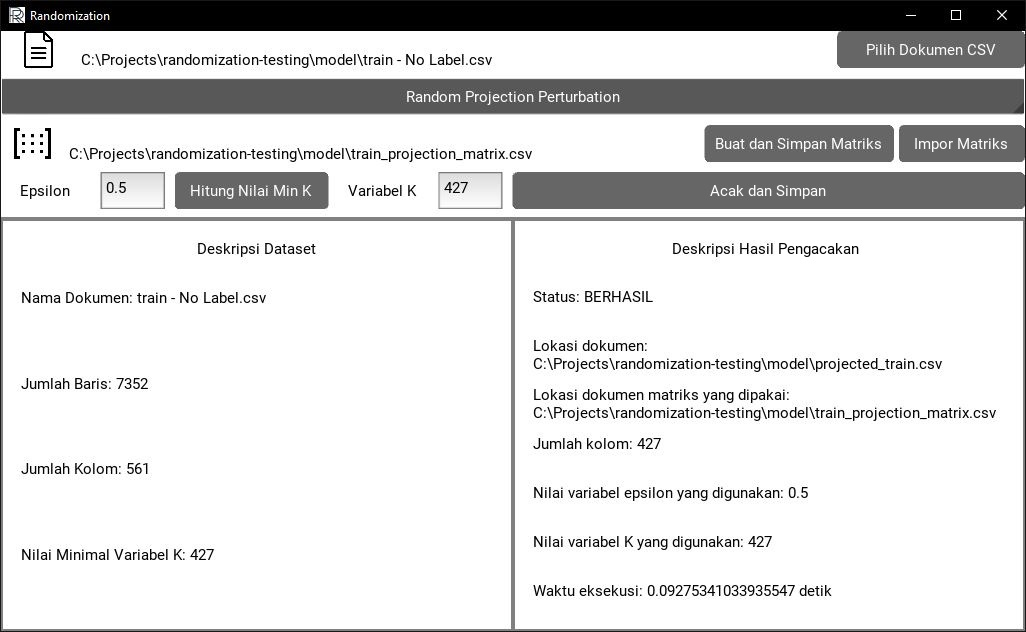
\includegraphics[scale=0.6]{antarmukahasilrandomisasi}
	\caption{Tampilan antarmuka deskripsi hasil randomisasi setelah perangkat berhasil melakukan randomisasi}
	\label{fig:antarmukahasilrandomisasi}
\end{figure}

\section{Pengujian Perangkat Lunak Fungsional}
\label{sec:pengujianfungsional}

Pengujian fungsional bertujuan untuk memastikan perangkat lunak randomisasi dapat menerapkan kedua teknik randomisasi yaitu \textit{Random Rotation Perturbation} dan \textit{Random Projection Perturbation} dengan baik terhadap dataset yang memenuhi syarat. Proses pengujian akan dilakukan dengan cara menerapkan kedua teknik tersebut dari awal memasukkan dataset sampai menghasilkan dataset yang telah dirandomisasi. Berikut pengujian pada setiap teknik randomisasi dengan menerapkan teknik penambangan data. Berikut pengujian pada setiap teknik randomisasi dengan menerapkan teknik penambangan data.

\subsection{Teknik \textit{Random Rotation Perturbation}}
\label{sec:rrp-fungsional}

Pengujian teknik \textit{Random Rotation Perturbation} akan menggunakan dataset \textit{mall\_customers} yang berisi informasi pribadi pelanggan sebuah mall. Dataset ini memiliki empat buah fitur yaitu jenis kelamin, umur, penghasilan, dan skor pengeluaran. Empat buah fitur tersebut akan dirandomisasi dan diharapkan hasilnya akan mengacak dataset sehingga nilai tiap fitur tersebut berbeda dari aslinya. Selain itu, matriks rotasi harus dapat disimpan dan digunakan kembali untuk lain kali. Dataset yang telah dirandomisasi juga diharapkan masih dapat diterapkan teknik penambangan data dengan hasil yang kualitasnya sama dengan dataset asli, pengujian untuk hal ini akan dilakukan pada bagian berikutnya yaitu pada pengujian eksperimental.

Pada teknik \textit{Random Rotation Perturbation} untuk merotasikan sebuah dataset diperlukan sebuah matriks rotasi dan translasi acak. Perangkat lunak diharapkan dapat membuat kedua matriks tersebut dan menyimpannya ke dalam sebuah dokumen \textit{commas-separated values}. Beberapa kolom pada dataset \textit{mall\_customers} harus dihilangkan terlebih dahulu agar hanya fitur (bersifat numerik) pada dataset tersebut saja yang terandomisasi. Dataset \textit{mall\_customers} mempunyai 3 buah fitur yang akan dirandomisasi, oleh karena itu matriks rotasi dan translasi acak yang dibuat perangkat lunak seharusnya berukuran \(3*3\) kecuali matriks translasi yang akan berukuran \(4*4\) karena matriks translasi mempunyai kolom terakhir tambahan yang dibutuhkan untuk melakukan tranformasi translasi. 

Pada pengujian yang dilakukan, perangkat lunak berhasil membuat kedua matriks acak tersebut dengan ukuran yang benar dan menyimpannya pada satu dokumen \textit{commas-separated values} yang isinya dapat dilihat pada Gambar~\ref{fig:mall_rotation_matrix}. Matriks rotasi dan translasi ini akan digunakan untuk menerapkan teknik \textit{Random Rotation Perturbation} terhadap dataset \textit{mall\_customers}. Perangkat lunak juga berhasil menggunakan ulang kedua matriks yang telah disimpan tersebut untuk menerapkan teknik \textit{Random Rotation Perturbation} terhadap dataset \textit{mall\_customers} dan hasilnya sama persis seperti hasil yang pertama kali. Kedua matriks tersebut juga dapat digunakan untuk data \textit{mall\_customers} yang lain dengan syarat masih memiliki jumlah fitur yang sama.

\begin{figure}
	\centering
	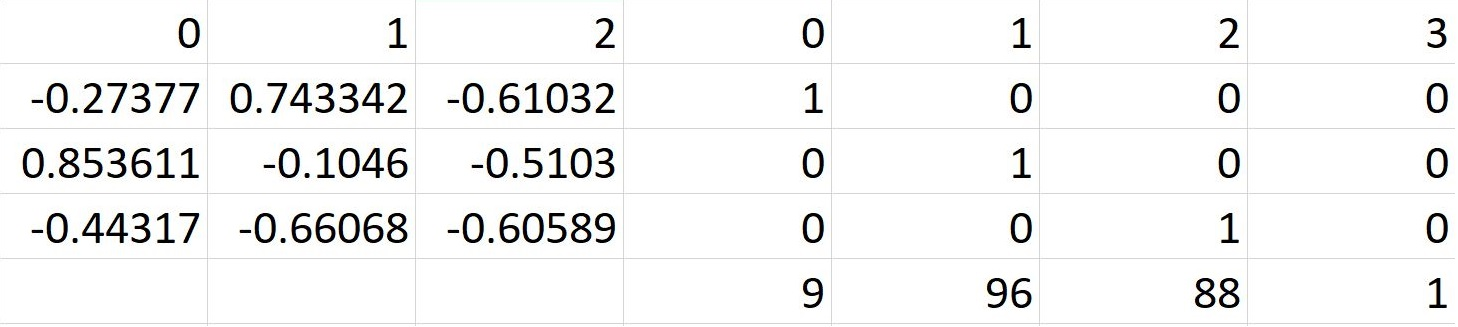
\includegraphics[scale=0.35]{mall_rotation_matrix}
	\caption{Matriks rotasi dan translasi acak yang dibuat perangkat lunak dan disimpan pada satu dokumen  \textit{commas-separated values}}
	\label{fig:mall_rotation_matrix}
\end{figure}

Berikut akan ditampilkan 20 baris pertama dataset asli dan dataset yang telah dirandomisasi masing-masing pada Gambar~\ref{fig:mall_customers_asli} dan Gambar~\ref{fig:rotated_mall_customers}. Dapat dilihat pada gambar tersebut, dataset setelah dirandomisasi memiliki nilai yang sangat berbeda dengan aslinya. Terlebih lagi jika diperhatikan, nilai yang sama pada beberapa baris di dataset asli tidak sama dengan dataset yang telah dirandomisasi pada baris yang sama seperti pada kolom \textit{insulin} baris 10 sampai 12 memiliki nilai 19 pada dataset asli tetapi pada dataset yang telah dirandomisasi ketiga baris tersebut memiliki nilai yang berbeda antara satu dengan yang lainnya. Dalam rangka untuk memastikan perangkat lunak berhasil dengan benar menerapkan teknik \textit{Random Rotation Perturbation} dengan matriks rotasi dan translasi yang sebelumnya sudah dibuat dan disimpan oleh perangkat lunak, perhitungan manual dilakukan terhadap dataset \textit{mall\_customers} dengan menggunakan matriks rotasi dan translasi tersebut. Perhitungan manual dan hasil akhirnya pada 20 baris pertama dapat dilihat masing-masing pada <<TODO>> dan <<TODO>>. Apabila dibandingkan hasil dari perangkat lunak dan perhitungan manual, dapat dilihat hasil dari perangkat lunak sama persis dengan hasil dari perhitungan manual. Oleh karena itu, dapat disimpulkan bahwa perangkat lunak sudah berfungsi dengan baik dan benar dalam menerapkan teknik \textit{Random Rotation Perturbation}.

\begin{figure}
	\centering
	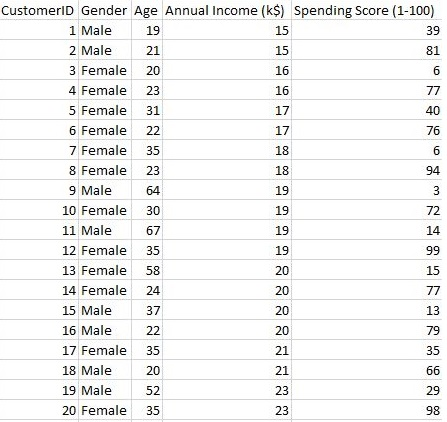
\includegraphics[scale=0.9]{mall_customers_asli}
	\caption{Dua puluh baris pertama dataset \textit{mall\_customers} asli}
	\label{fig:mall_customers_asli}
\end{figure}

\begin{figure}
	\centering
	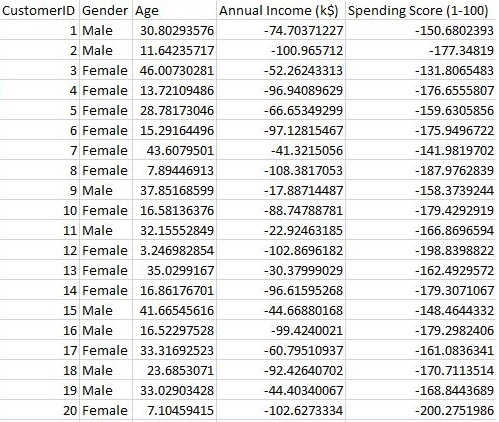
\includegraphics[scale=0.9]{rotated_mall_customers}
	\caption{Dua puluh baris pertama dataset \textit{mall\_customers} setelah dirandomisasi}
	\label{fig:rotated_mall_customers}
\end{figure}

\subsection{Teknik \textit{Random Projection Perturbation}}
\label{sec:rpp-fungsional}

Pengujian teknik \textit{Random Projection Perturbation} akan menggunakan dataset \textit{mobile\_sensor} yang berisi data sensor \textit{smartphone} banyak orang yang sedang melakukan aktivitas tertentu seperti berdiri, duduk, berjalan, berjalan menanjak, berjalan menurun, dan lain-lain. Dataset ini memiliki 561 buah fitur dan sebuah label. Seluruh fitur tersebut akan dirandomisasi dan diharapkan hasilnya akan mengacak dataset sehingga nilai tiap fitur tersebut berbeda dari aslinya. Dataset yang telah dirandomisasi juga diharapkan masih dapat diterapkan teknik penambangan data dengan hasil yang kualitasnya mirip dengan dataset asli, pengujian untuk hal ini akan dilakukan pada bagian berikutnya yaitu pada pengujian eksperimental.

Label pada dataset \textit{mobile\_sensor} yang ingin dirandomisasi harus dihilangkan terlebih dahulu agar hanya fitur (bersifat numerik) pada dataset tersebut saja yang terandomisasi. Nilai variabel Epsilon yang dipilih pada pengujian ini adalah sebesar 0.52 dan dengan nilai variabel \textit{Epsilon} tersebut nilai minimal variabel \textit{k} adalah sebesar 418.0905. Pada pengujian ini perangkat lunak berhasil menghitung dengan benar nilai minimal variabel \textit{k} yaitu sebesar 418 dengan dataset \textit{mobile\_sensor} dan nilai variabel Epsilon sebesar 0.52. Berikut ini adalah perhitungan manual nilai minimal variabel \textit{k} dengan nilai variabel Epsilon sebesar 0.52 dan jumlah baris pada dataset sebanyak 10299 baris.
\begin{align*}
	k &= \frac{4\ln{n}}{\frac{\epsilon^{2}}{2}-\frac{\epsilon^{3}}{3}} \\
	&= \frac{4\ln{10299}}{\frac{0.52^{2}}{2}-\frac{0.52^{3}}{3}} \\
	&= \frac{36.9592}{0.1352-0.0468} \\
	&= 418.0905
\end{align*}

Pada teknik \textit{Random Projection Perturbation} untuk memproyeksikan sebuah dataset diperlukan sebuah matriks proyeksi acak. Perangkat lunak diharapkan dapat membuat sebuah matriks proyeksi acak dan menyimpannya ke dalam sebuah dokumen \textit{commas-separated values}. Dataset \textit{mobile\_sensor} memiliki 561 buah fitur yang akan dirandomisasi dan sesuai dengan nilai minimal vaiabel \textit{k} yang sudah dihitung sebelumnya yaitu sebesar 418 maka ditentukan nilai \textit{k} yang dipakai pada pengujian ini adalah sebesar 427. Oleh karena itu, matriks proyeksi acak yang dibuat perangkat lunak seharusnya berukuran \(427*427\).

Pada pengujian yang dilakukan, perangkat lunak berhasil membuat matriks proyeksi acak tersebut dengan ukuran yang benar dan menyimpannya pada sebuah dokumen \textit{commas-separated values} yang 10 kolom pertama pada 20 baris pertamanya dapat dilihat pada Gambar~\ref{fig:mobile_sensor_projection_matrix}. Matriks proyeksi ini akan digunakan untuk menerapkan teknik \textit{Random Projection Perturbation} terhadap dataset \textit{mobile\_sensor}. Perangkat lunak juga berhasil menggunakan ulang matriks yang telah disimpan tersebut untuk menerapkan teknik \textit{Random Projection Perturbation} terhadap dataset \textit{mobile\_sensor} dan hasilnya sama persis seperti hasil yang pertama kali. Matriks proyeksi tersebut juga dapat digunakan untuk data \textit{mobile\_sensor} yang lain dengan syarat masih memiliki jumlah fitur yang sama dan dengan penambahan data tersebut, nilai minimal variabel \textit{k} harus tetap lebih kurang atau sama dengan nilai \textit{k} yang dipilih. Persyaratan tersebut didasarkan oleh sifat pada teknik \textit{Random Projection Perturbation} yaitu nilai minimal variabel \textit{k} berbanding lurus dengan banyaknya data.

\begin{figure}
	\centering
	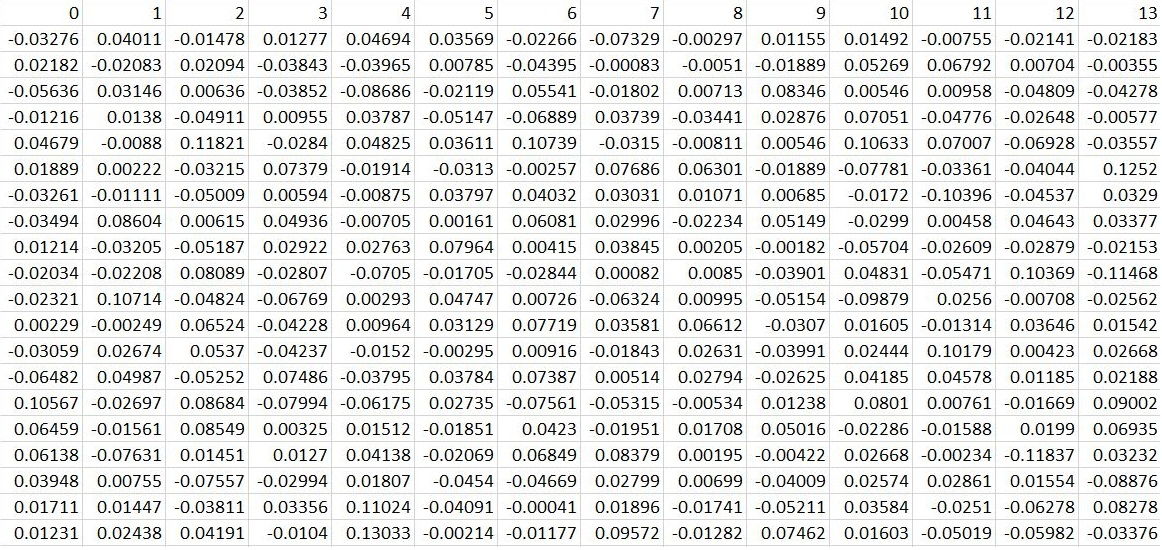
\includegraphics[scale=0.45]{mobile_sensor_projection_matrix}
	\caption{Matriks proyeksi acak yang dibuat perangkat lunak dan disimpan pada sebuah dokumen  \textit{commas-separated values}}
	\label{fig:mobile_sensor_projection_matrix}
\end{figure}

Berikut akan ditampilkan 7 fitur terakhir serta label pada 20 baris pertama dataset asli dan dataset yang telah dirandomisasi masing-masing pada Gambar~\ref{fig:mobile_sensor_asli} dan Gambar~\ref{fig:projected_mobile_sensor}. Dapat dilihat pada gambar tersebut, dataset setelah dirandomisasi memiliki nilai yang berbeda dengan aslinya. Terlebih lagi setiap fitur pada dataset yang telah dirandomisasi tidak diketahui arti dari setiap fitur tersebut apa karena sudah tereduksi sehingga seluruh fitur pada dataset asli tercampur secara acak dan terproyeksikan ke dalam 427 fitur yang ada pada dataset yang telah dirandomisasi. Dalam rangka untuk memastikan perangkat lunak berhasil dengan benar menerapkan teknik \textit{Random Projection Perturbation} dengan matriks proyeksi acak yang sebelumnya sudah dibuat dan disimpan oleh perangkat lunak, perhitungan manual dilakukan terhadap dataset \textit{mobile\_sensor} dengan menggunakan matriks proyeksi tersebut. Perhitungan manual dan hasil akhirnya (7 kolom terakhir pada 20 baris pertama) dapat dilihat masing-masing pada <<TODO>> dan <<TODO>>. Apabila dibandingkan hasil dari perangkat lunak dan perhitungan manual, dapat dilihat hasil dari perangkat lunak sama persis dengan hasil dari perhitungan manual. Oleh karena itu, dapat disimpulkan bahwa perangkat lunak sudah berfungsi dengan baik dan benar dalam menerapkan teknik \textit{Random Projection Perturbation}.

\begin{figure}
	\centering
	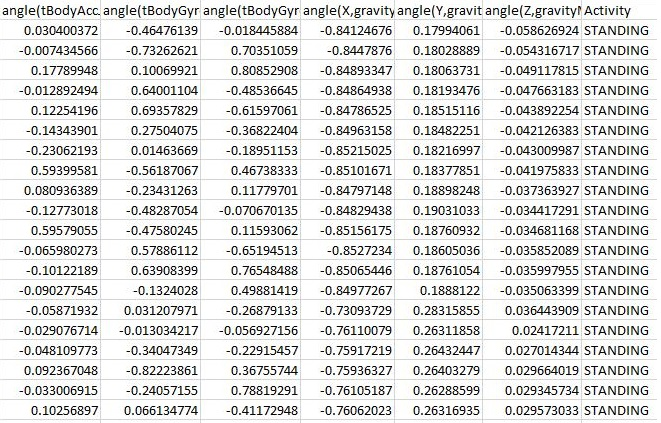
\includegraphics[scale=0.9]{mobile_sensor_asli}
	\caption{Dua puluh baris terakhir dataset \textit{mobile\_sensor} yang asli}
	\label{fig:mobile_sensor_asli}
\end{figure}

\begin{figure}
	\centering
	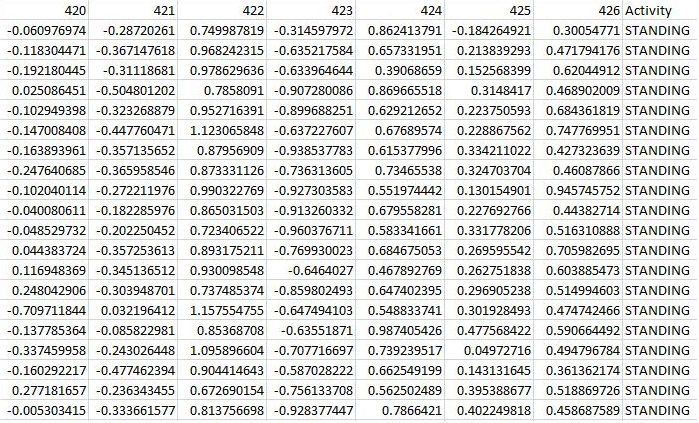
\includegraphics[scale=0.8]{projected_mobile_sensor}
	\caption{Dua puluh baris terakhir dataset \textit{mobile\_sensor} setelah dirandomisasi}
	\label{fig:projected_mobile_sensor}
\end{figure}

Dalam rangka memastikan lebih lagi apakah perangkat lunak menerapkan teknik \textit{Random Projection Perturbation} dengan akurat, perangkat lunak pengujian dibuat untuk menguji jarak Euclidean dari setiap titik pada dataset terhadap setiap titik lainnya. Pengujian dilakukan dengan menggunakan pertidaksamaan rentang jarak Euclidean berikut untuk menguji apakah jarak Euclidean pada dataset yang telah dirandomisasi mempunyai \textit{error} yang lebih besar dari harapan pengguna. Hasil dari perangkat lunak diharapkan (dataset yang telah dirandomisasi) memenuhi pertidaksamaan berikut ini.

\begin{equation}
	(1-eps)||u - v||^{2}<||p(u) - p(v)||^{2}<(1+eps)||u - v||^{2}
\end{equation}

Pada pengujian ini, dengan nilai variabel Epsilon sebesar 0.52 pertidaksamaan tersebut terpenuhi pada seluruh data yang ada pada dataset. Ada salah satu kasus saat pertidaksamaan tersebut tidak terpenuhi yaitu apabila nilai variabel Epsilon ditentukan sebesar 0.4. Salah satu jarak Euclidean yang melanggar pertidaksamaan tersebut adalah baris 473 dengan baris 1306 yang memiliki jarak Euclidean sebesar 8.167734238223167 pada dataset asli dan 9.723888530285468 pada dataset yang telah dirandomisasi. Pengujian ini membuktikan bahwa perangkat lunak berhasil menerapkan teknik \textit{Random Projection Perturbation} dengan akurat sesuai batas \textit{error} yang ditentukan pengguna.

\section{Pengujian Eksperimental}
\label{sec:pengujianeksperimental}

Pengujian eksperimental bertujuan untuk menguji kualitas hasil dari perangkat lunak randomisasi pada kedua teknik randomisasi dan membandingkan kualitas hasil randomisasi dari kedua teknik tersebut pada penambangan data. Pengujian akan dilakukan dalam dua bagian yaitu pengujian kualitas teknik randomisasi untuk penambangan data klasifikasi dan pengujian kualitas teknik randomisasi untuk penambangan data \textit{clustering}. Pada setiap bagian tersebut akan dibagi lagi menjadi tiga bagian yaitu pengujian teknik \textit{Random Rotation Perturbation}, pengujian teknik \textit{Random Projection Perturbation}, dan pengujian untuk membandingkan kedua teknik randomisasi tersebut. Pengujian akan dilakukan dengan menggunakan program pengujian yang menerapkan teknik penambangan data yang telah dibuat pada bahasa pemograman Python dan didukung oleh perangkat lunak \textit{Spyder} untuk menampilkan visualisasi hasil penambangan data.

\subsection{Penambangan Data Klasifikasi}
\label{sec:pengujian-klasifikasi}
Pengujian dengan penambangan data klasifikasi akan berpusat pada pembuatan model dengan dataset asli dan dataset yang telah dirandomisasi dan membandingkan kualitas model tersebut. Teknik penambangan data klasifikasi yang digunakan adalah \textit{K-nearest neighbors}. Berikut hasil pengujian eksperimental yang telah dilakukan.

\subsubsection{\textit{Random Rotation Perturbation}}
\label{sec:pengujian-klasifikasi-rrp}

Pengujian teknik \textit{Random Rotation Perturbation} untuk penambangan data klasifikasi dengan algoritma \textit{K-nearest neighbors} akan dilakukan dengan dataset \textit{diabetes} yang dapat dilihat 20 baris pertamanya pada Gambar~\ref{fig:diabetes_asli}. Dataset ini dirandomisasi dengan teknik \textit{Random Rotation Perturbation} dan hasil randomisasi dapat dilihat pada Gambar~\ref{fig:rotated_diabetes}. Dengan kedua dataset tersebut, dilakukan penambangan data terhadap kedua dataset tersebut dan dihasilkan berbagai macam informasi yang dapat dibandingkan. Berikut adalah hasil pengujian dan penjelasannya.

\begin{figure}
	\centering
	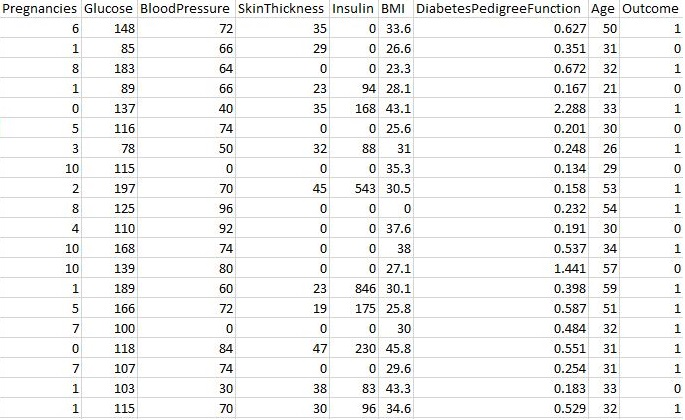
\includegraphics[scale=0.9]{diabetes_asli}
	\caption{Dua puluh baris pertama dataset \textit{diabetes} asli}
	\label{fig:diabetes_asli}
\end{figure}

\begin{figure}
	\centering
	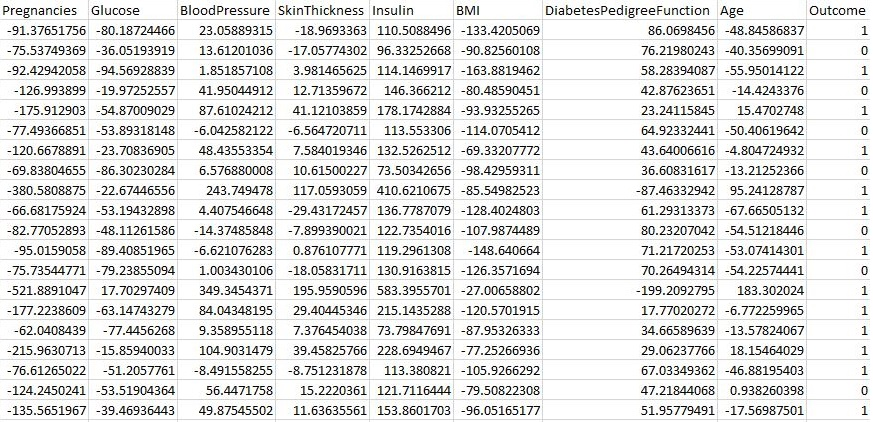
\includegraphics[scale=0.71]{rotated_diabetes}
	\caption{Dua puluh baris pertama dataset \textit{diabetes} setelah dirandomisasi}
	\label{fig:rotated_diabetes}
\end{figure}

\begin{itemize}
	\item Pada dataset \textit{diabetes}, jumlah kasus diabetes atau dengan kata lain distribusi label pada dataset ini dapat dilihat pada Gambar~\ref{fig:distribusi_label_diabetes}. Dataset \textit{diabetes} asli dan dataset \textit{diabetes} yang telah dirandomisasi tentunya memiliki distribusi label yang sama karena label tidak dirandomisasi sehingga tidak berubah.

	\begin{figure}
		\centering
		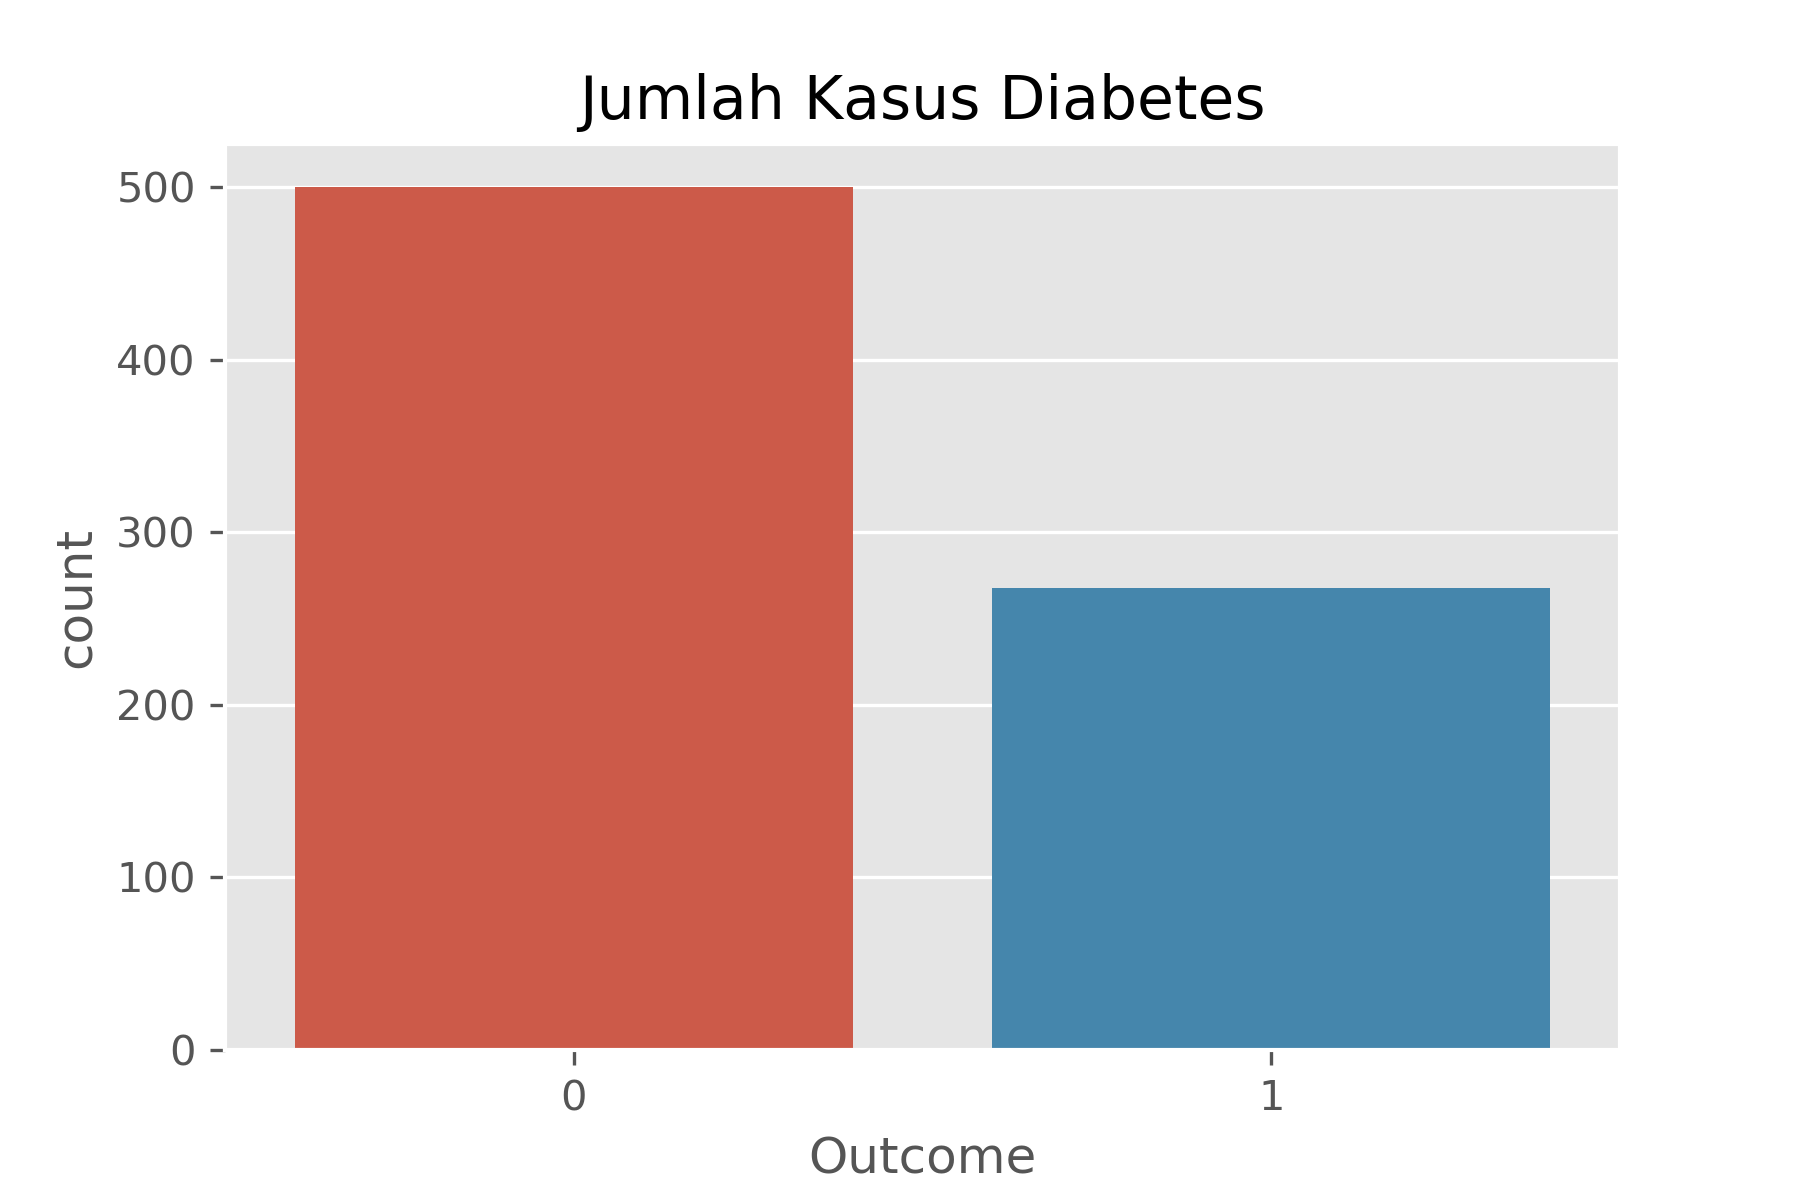
\includegraphics[scale=1]{distribusi_label_diabetes}
		\caption{Histogram distribusi label dataset \textit{diabetes}}
		\label{fig:distribusi_label_diabetes}
	\end{figure}
	\item Properti-properti pada dataset \textit{diabetes} asli dapat dilihat pada Tabel~\ref{table:properti-diabetes-asli-1} dan Tabel~\ref{table:properti-diabetes-asli-2}. Sementara untuk dataset \textit{diabetes} yang telah dirandomisasi dapat dilihat pada Tabel~\ref{table:properti-diabetes-randomisasi-1} dan Tabel~\ref{table:properti-diabetes-randomisasi-2}. Jika dilihat pada keempat tabel tersebut, seluruh properti pada dataset yang telah dirandomisasi mempunyai nilai yang berbeda kecuali jumlah baris (\textit{count}) dan kolom label (\textit{Outcome}). Hal ini menunjukkan selain nilai pada setiap data, teknik \textit{Random Rotation Perturbation} juga mengacak bermacam properti data seperti rata-rata, standar deviasi, batas bawah dan batas atas nilai pada data.

	\begin{table}
		\centering
		\caption{Properti-properti pada dataset \textit{diabetes} asli}
		\begin{tabular}{l|lllll}
			\hline
			 & Pregnancies & Glucose & BloodPressure & SkinThickness & Insulin \\ \hline
			count & 768.000000 & 768.000000 & 768.000000 & 768.000000 & 768.000000 \\
			mean & 3.845052 & 120.894531 & 69.105469 & 20.536458 & 79.799479 \\
			std & 3.369578 & 31.972618 & 19.355807 & 15.952218 & 115.244002 \\
			min & 0.000000 & 0.000000 & 0.000000 & 0.000000 & 0.000000 \\
			25\% & 1.000000 & 99.000000 & 62.000000 & 0.000000 & 0.000000 \\
			50\% & 3.000000 & 117.000000 & 72.000000 & 23.000000 & 30.500000 \\
			75\% & 6.000000 & 140.250000 & 80.000000 & 32.000000 & 127.250000 \\
			max & 17.000000 & 199.000000 & 122.000000 & 99.000000 & 846.000000 \\
			\hline
		\end{tabular}
		\label{table:properti-diabetes-asli-1}
	\end{table}
	
	\begin{table}
		\centering
		\caption{Properti-properti pada dataset \textit{diabetes} asli}
		\begin{tabular}{l|llll}
			\hline
			 & BMI & DiabetesPedigreeFunction & Age & Outcome \\ \hline
			count & 768.000000 & 768.000000 & 768.000000 & 768.000000 \\
			mean & 31.992578 & 0.471876 & 33.240885 & 0.348958 \\
			std & 7.884160 & 0.331329 & 11.760232 & 0.476951 \\
			min & 0.000000 & 0.078000 & 21.000000 & 0.000000 \\
			25\% & 27.300000 & 0.243750 & 24.000000 & 0.000000\\
			50\% & 32.000000 & 0.372500 & 29.000000 & 0.000000 \\
			75\% & 36.600000 & 0.626250 & 41.000000 & 1.000000 \\
			max & 67.100000 & 2.420000 & 81.000000 & 1.000000 \\
			\hline
		\end{tabular}
		\label{table:properti-diabetes-asli-2}
	\end{table}
	
	\begin{table}
		\centering
		\caption{Properti-properti pada dataset \textit{diabetes} yang telah dirandomisasi}
		\begin{tabular}{l|lllll}
			\hline
			 & Pregnancies & Glucose & BloodPressure & SkinThickness & Insulin \\ \hline
			count & 768.000000 & 768.000000 & 768.000000 & 768.000000 & 768.000000 \\
			mean & -125.296036 & -46.928128 & 38.476869 & 8.970500 & 149.05599 \\
			std & 65.385296 & 24.314318 & 48.951102 & 29.325358 & 64.087311 \\
			min & -521.889105 & -130.730268 & -21.449526 & -40.186125 & 60.899387\\
			25\% & -156.640887 & -61.988042 & 4.264140 & -9.412375 & 109.984343 \\
			50\% & -102.169672 & -44.481520 & 21.426488 & 2.512069 & 127.946623 \\
			75\% & -79.991828 & -30.399185 & 61.569078 & 20.287410 & 171.374079 \\
			max & -43.084371 & 29.654467 & 349.345437 & 195.959060 & 583.395570 \\
			\hline
		\end{tabular}
		\label{table:properti-diabetes-randomisasi-1}
	\end{table}
	
	\begin{table}
		\centering
		\caption{Properti-properti pada dataset \textit{diabetes} yang telah dirandomisasi}
		\begin{tabular}{l|llll}
			\hline
			 & BMI & DiabetesPedigreeFunction & Age & Outcome \\ \hline
			count & 768.000000 & 768.000000 & 768.000000 & 768.000000 \\
			mean & -103.101329 & 50.477502 & -23.129061 & 0.348958 \\
			std & 24.146554 & 35.533157 & 32.695887 & 0.476951  \\
			min & -176.332307 & -199.209279 & -74.182020 & 0.000000 \\
			25\% & -116.872237 & 35.049918 & -46.748389 & 0.000000 \\
			50\% & -101.458852 & 58.320138 & -28.463990 & 0.000000 \\
			75\% & -86.757613 & 73.320823 & -9.757361 & 1.000000 \\
			max & -22.156712 & 116.151884 & 183.302024 & 1.000000 \\
			\hline
		\end{tabular}
		\label{table:properti-diabetes-randomisasi-2}
	\end{table}
	\item Pada Gambar~\ref{fig:distribusi_kolom_diabetes_asli} terdapat \textit{scatter plot} antara satu fitur dengan fitur lainnya dan pada pada dataset asli. Sementara pada dataset yang telah dirandomisasi dapat dilihat pada Gambar~\ref{fig:distribusi_kolom_diabetes_randomisasi}. Dapat terlihat pada kedua gambar tersebut, lokasi pada titik-titik pada seluruh scatter plot berbeda. Hal ini menunjukkan teknik \textit{Random Rotation Perturbation} berhasil mengacak dengan baik setiap nilai yang ada dengan rotasi sehingga visualisasi seperti ini akan terlihat acak karena dataset dirotasi pada dimensi yang lebih besar.

	\begin{figure}
		\centering
		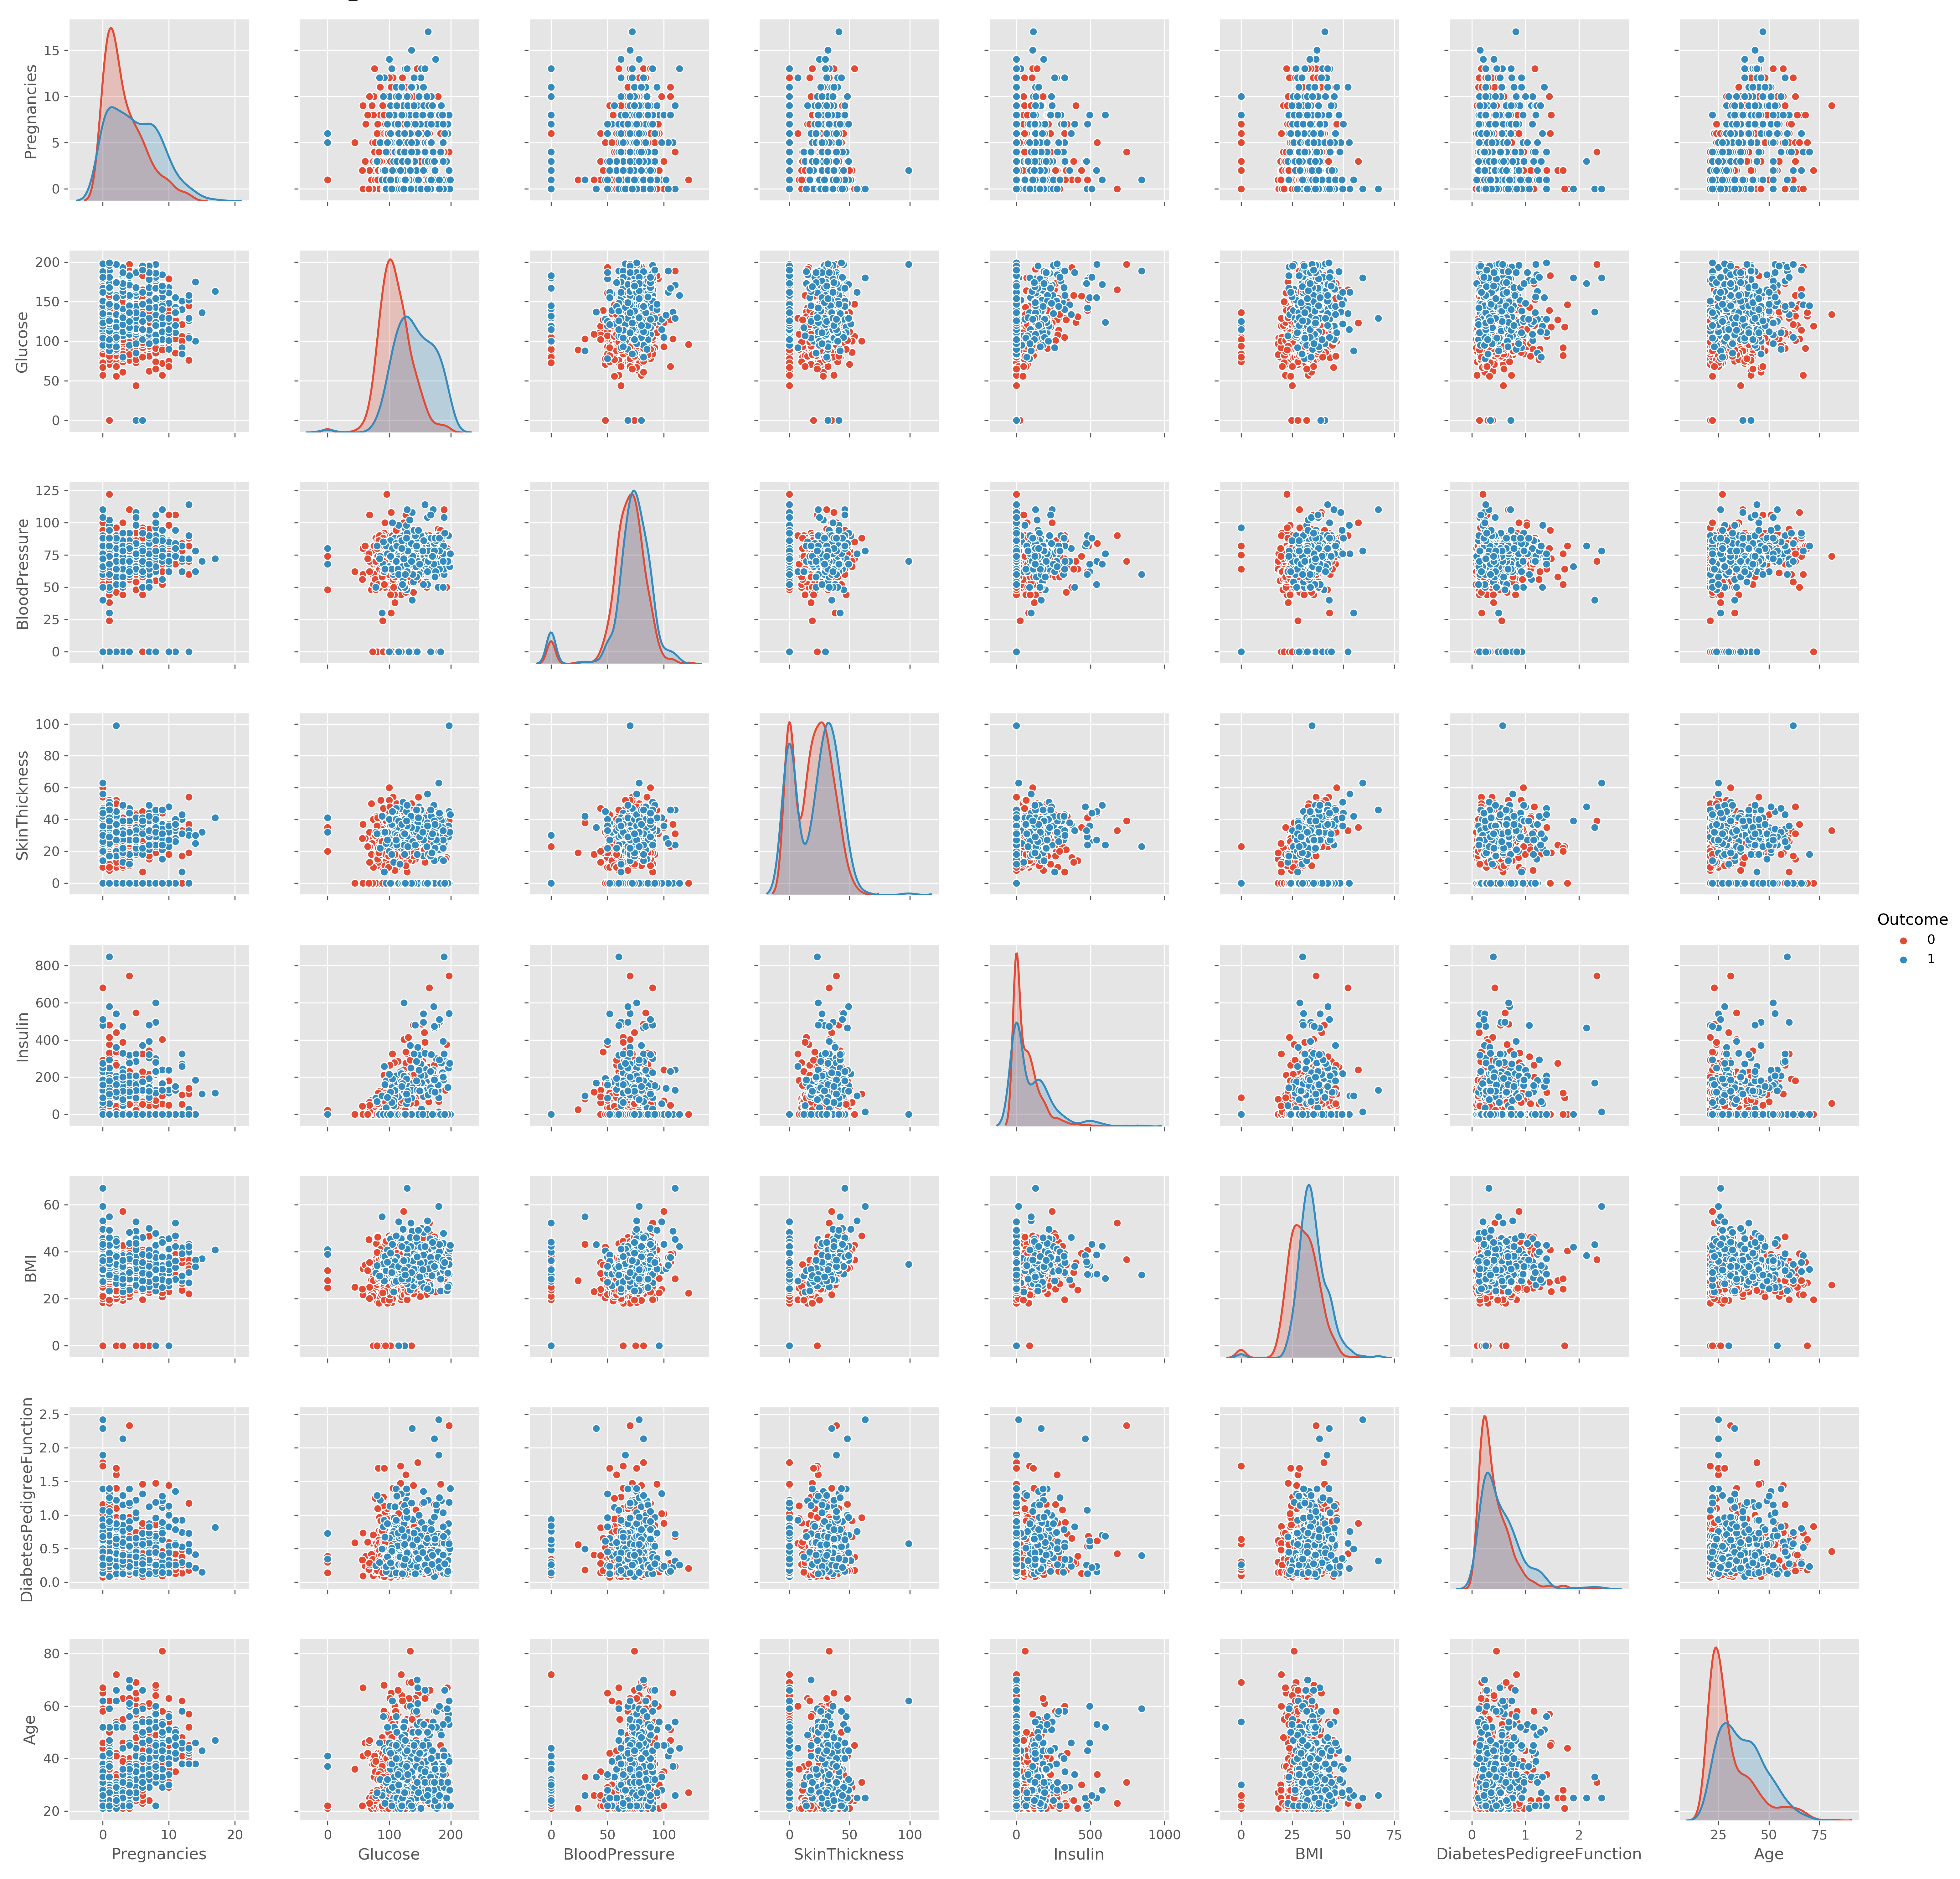
\includegraphics[scale=0.3]{distribusi_kolom_diabetes_asli}
		\caption{\textit{Scatter plot} antara seluruh fitur pada dataset \textit{diabetes} yang asli}
		\label{fig:distribusi_kolom_diabetes_asli}
	\end{figure}
	
	\begin{figure}
		\centering
		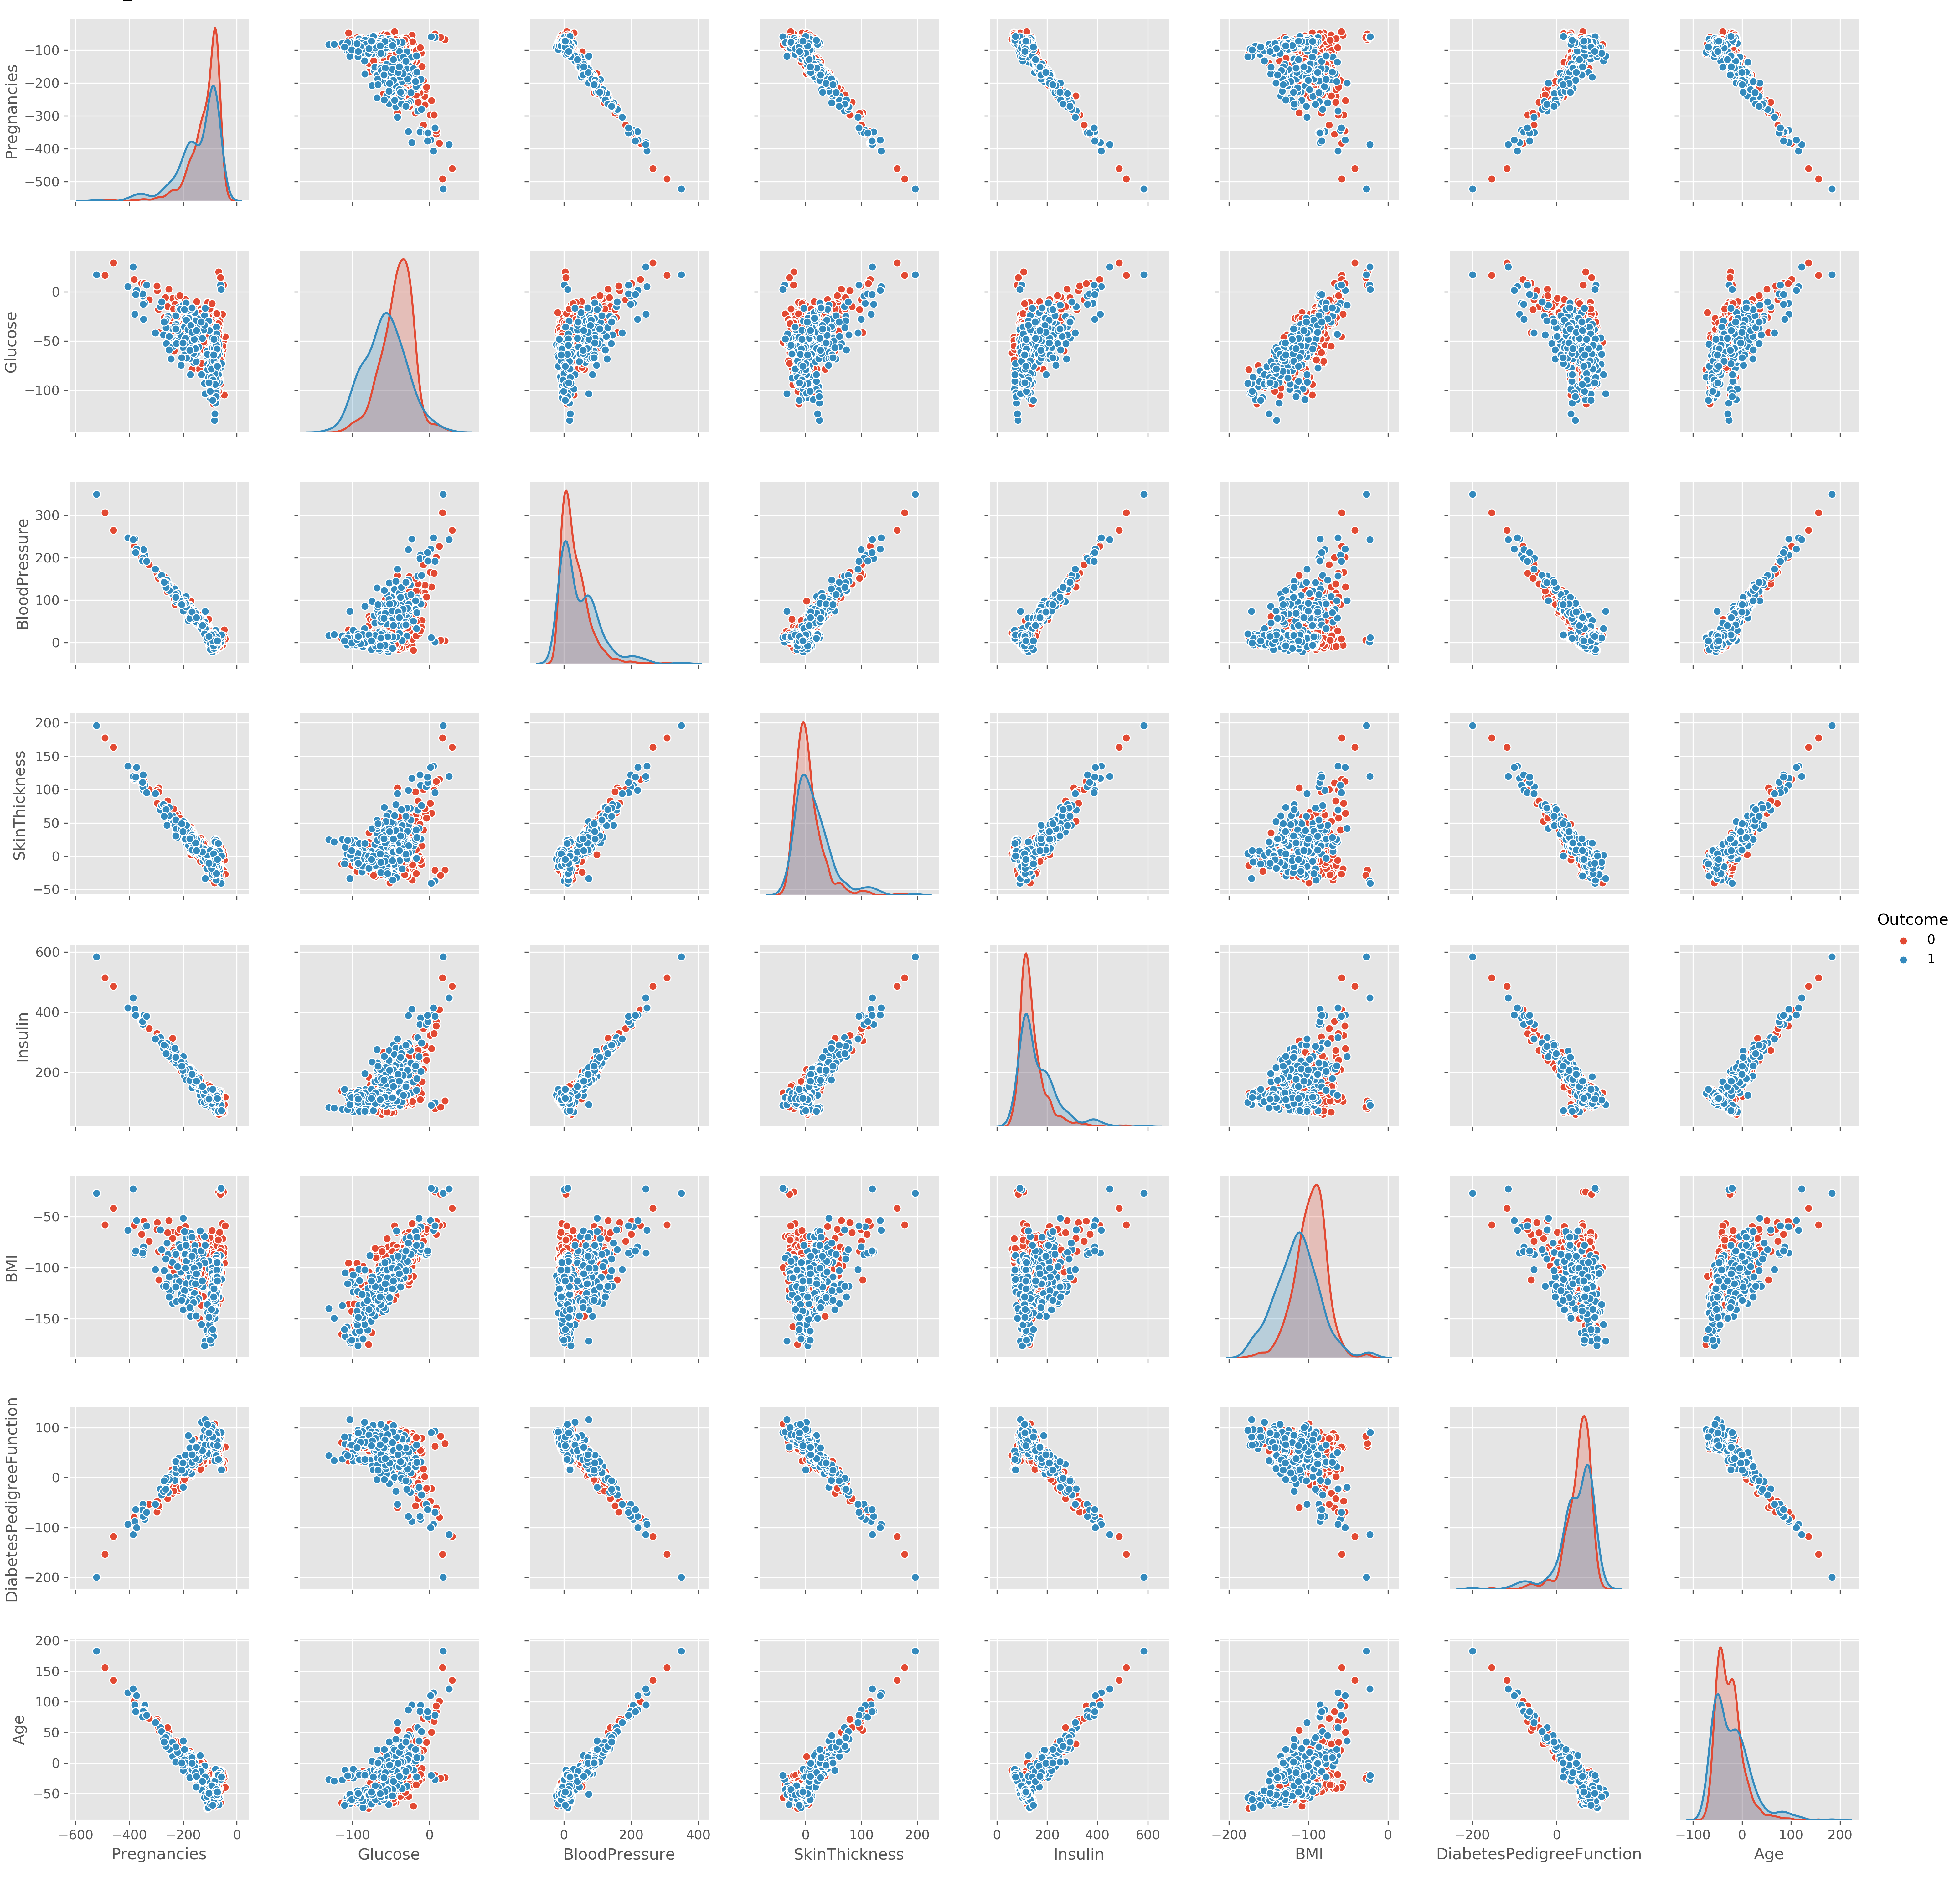
\includegraphics[scale=0.3]{distribusi_kolom_diabetes_randomisasi}
		\caption{\textit{Scatter plot} antara seluruh fitur pada dataset \textit{diabetes} yang telah dirandomisasi}
		\label{fig:distribusi_kolom_diabetes_randomisasi}
	\end{figure}
	\item Pada Gambar~\ref{fig:heatmap_diabetes} dapat dilihat korelasi antara satu fitur dengan fitur lainnya pada dataset asli dan dataset yang telah dirandomisasi. Apabila dibandingkan korelasi antar fitur pada dataset randomisasi sangat berbeda dengan dataset asli, bahkan tidak terlihat ada indikasi kesamaan atau ada properti pada dataset asli yang sama dengan dataset randomisasi. Hal ini menunjukkan teknik \textit{Random Rotation Perturbation} mengacak setiap nilai pada data tanpa menjaga properti lain selain jarak Euclidean.

	\begin{figure}
		\centering
		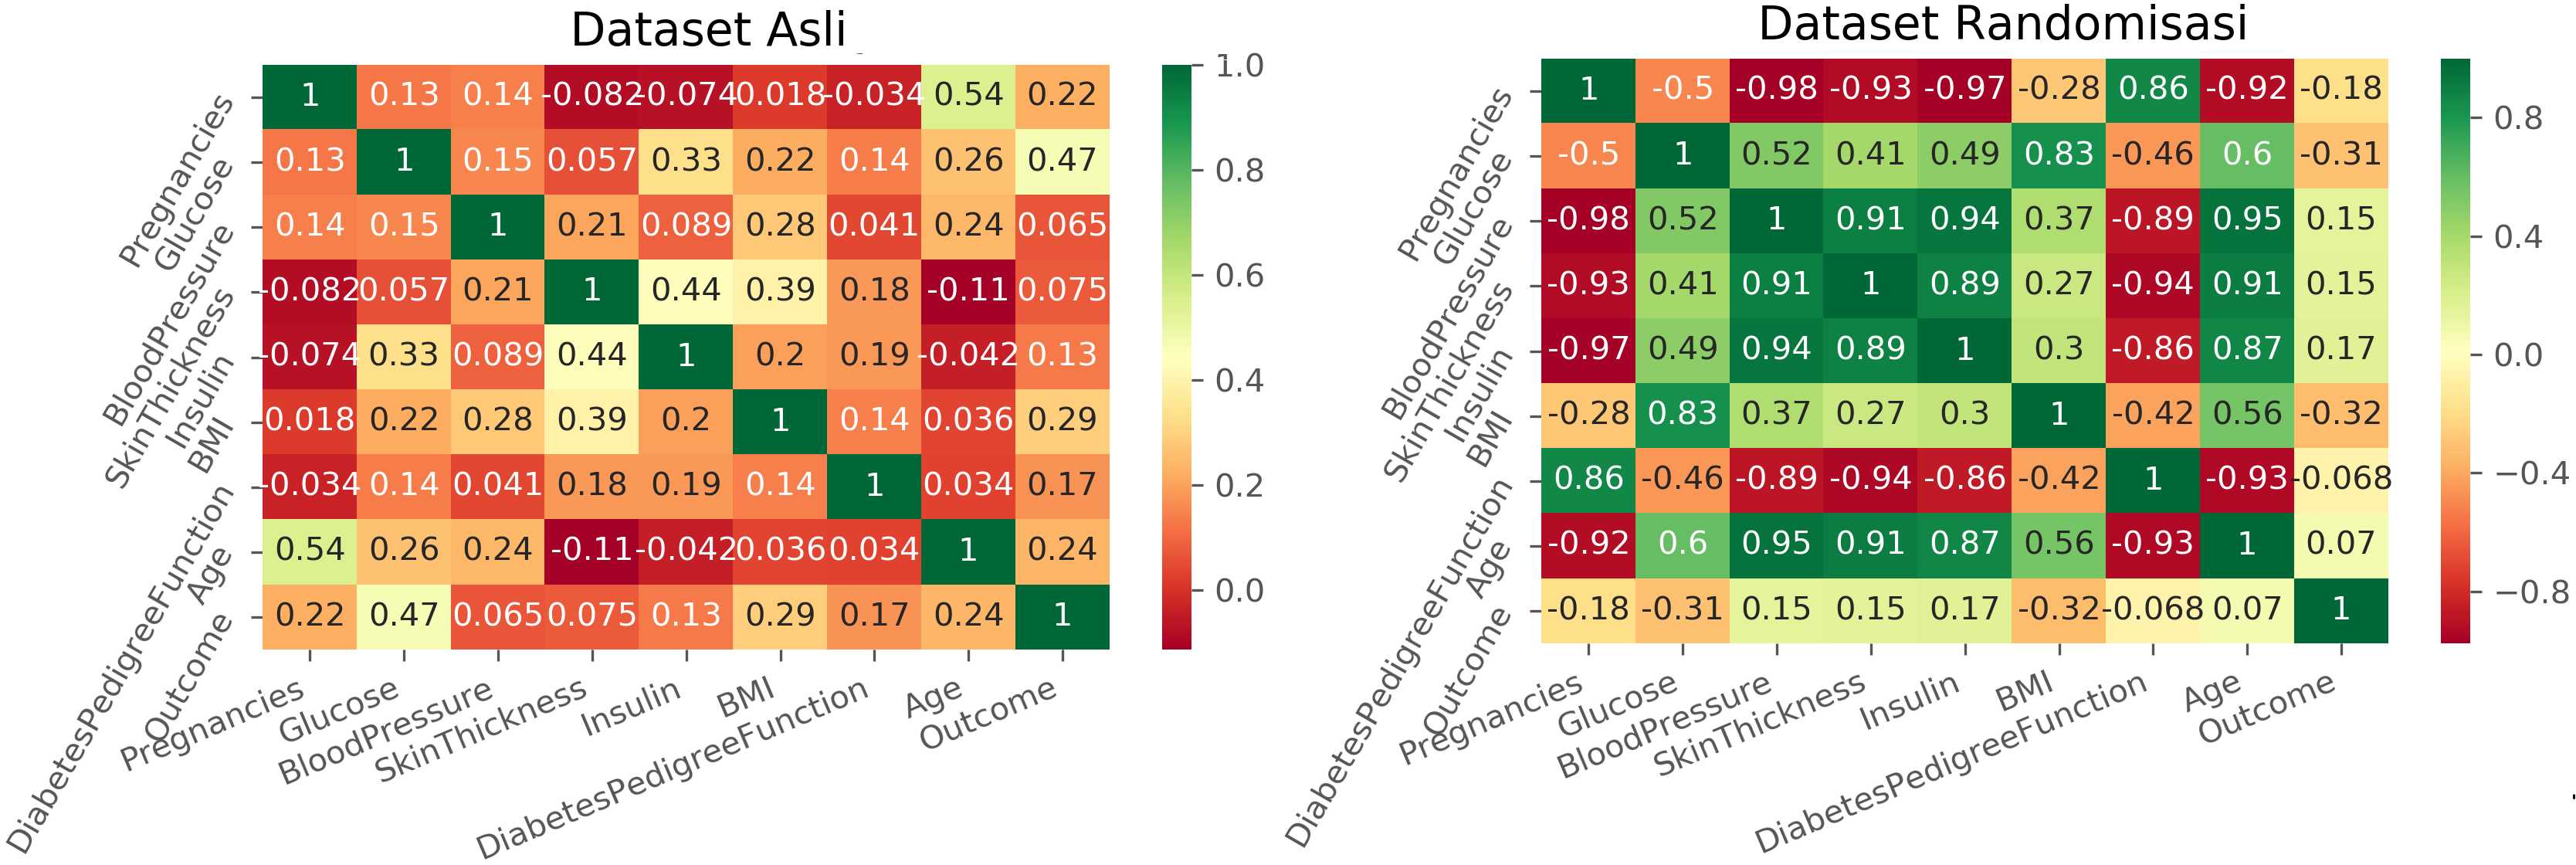
\includegraphics[scale=0.185]{heatmap_diabetes}
		\caption{\textit{Heatmap} korelasi antar fitur pada dataset \textit{diabetes}}
		\label{fig:heatmap_diabetes}
	\end{figure}
	\item Teknik penambangan data \textit{K-nearest Neighbors} diterapkan menggunakan delapan buah fitur yang ada untuk menguji apakah dataset asli dan dataset yang telah dirandomisasi mempunyai akurasi model klasifikasi yang sama persis. Pengujian tersebut didasarkan pada sifat dari teknik \textit{Random Rotation Perturbation} yang menjamin jarak Euclidean setiap titik tidak berubah sama sekali. Dataset akan dibagi dua menjadi \textit{train set} dan \textit{test set} yang masing-masing berguna untuk melatih model dan menghitung akurasi model. Akurasi akan dihitung pada setiap jumlah tetangga (nilai \textit{k}) dari 1 sampai 20. Implementasi kode teknik penambangan data ini diterapkan dengan bahasa pemograman Python dan dibantu oleh \textit{library} Scikit-learn. Pada Gambar~\ref{fig:plot_akurasi_diabetes} dapat dilihat grafik akurasi model \textit{K-nearest Neighbors} dalam memprediksi label \textit{training set} dan \textit{test set} pada dataset asli dan dataset yang telah dirandomisasi. Apabila dibandingkan, kedua grafik tersebut terlihat memiliki nilai akurasi yang sama persis untuk setiap nilai \textit{k}. 

	\begin{figure}
		\centering
		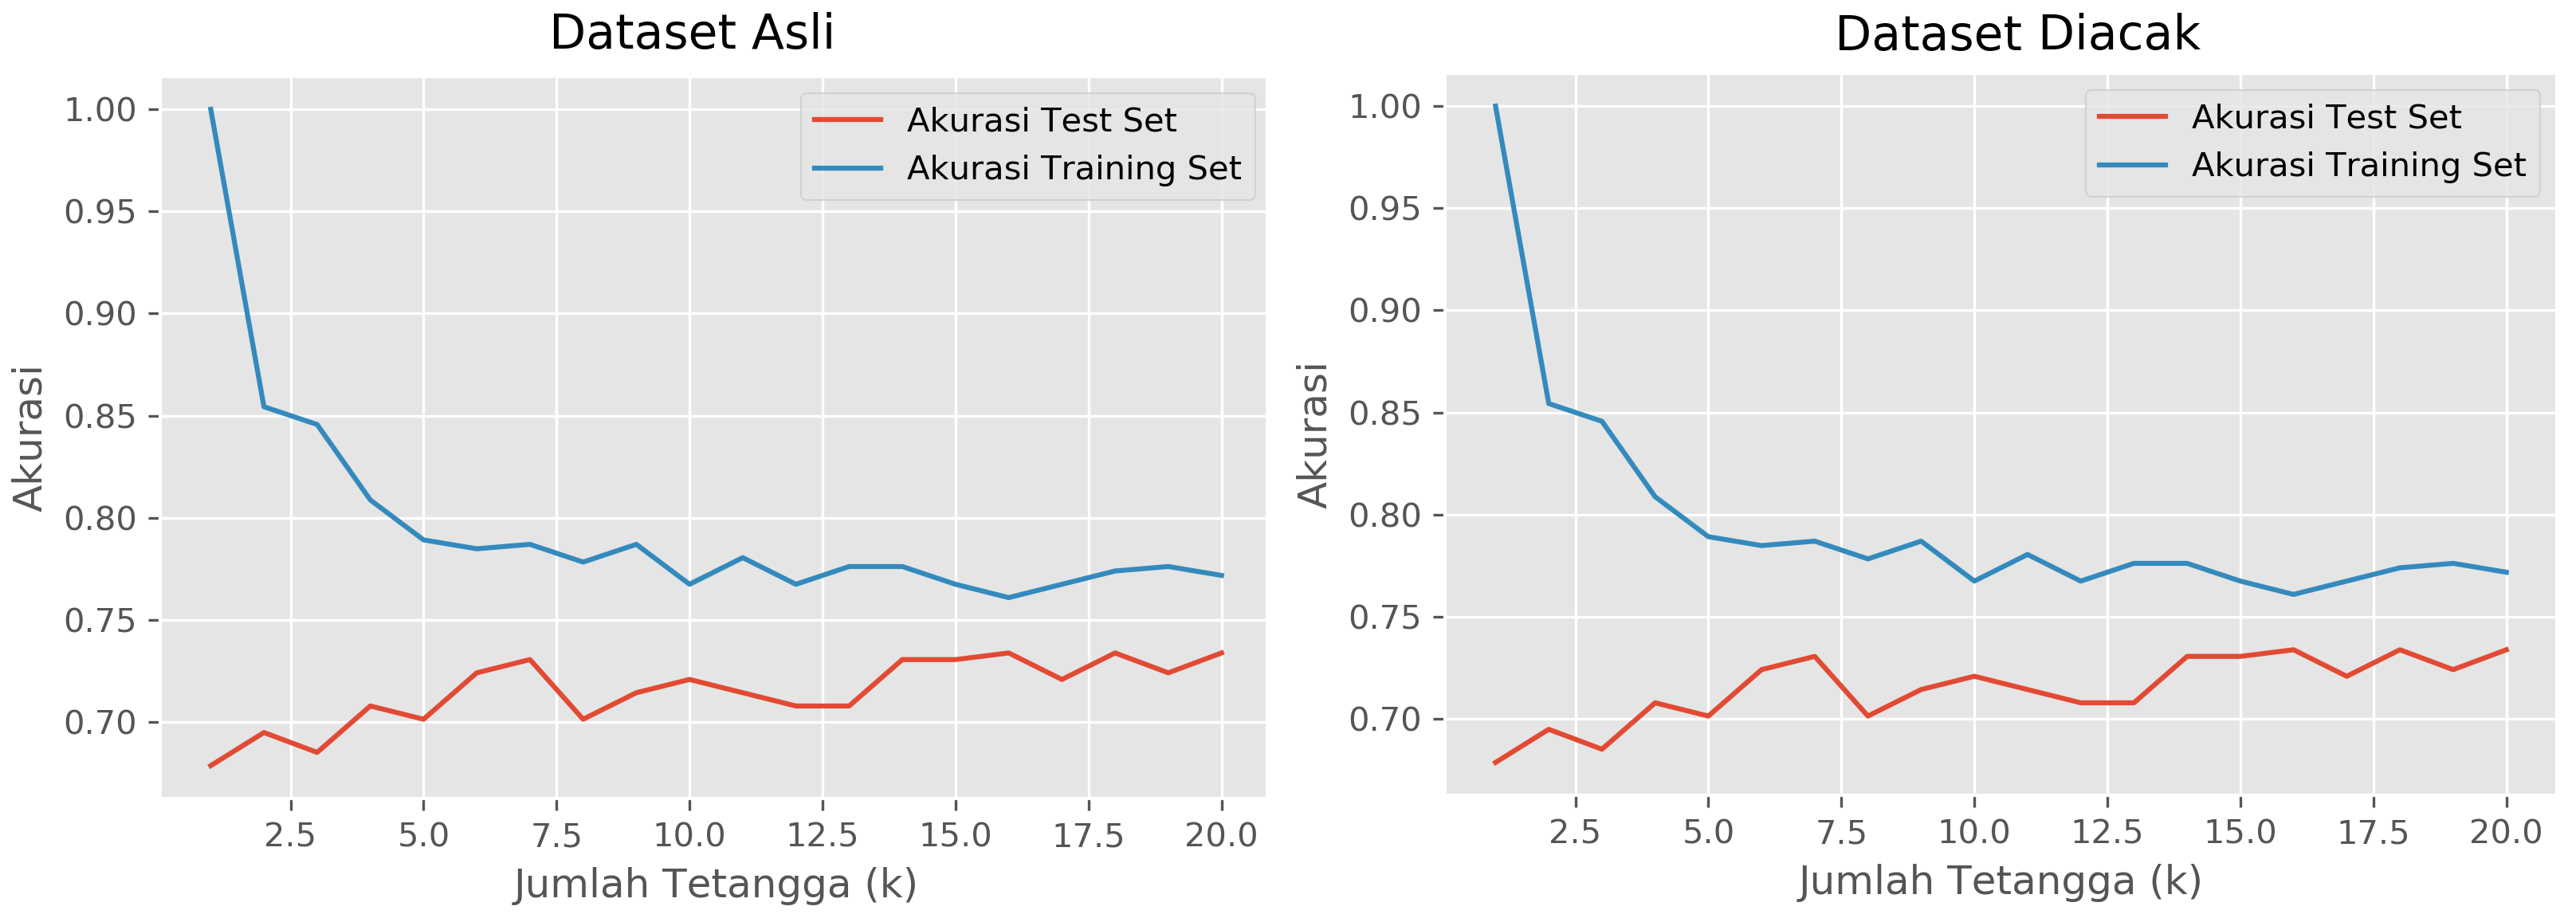
\includegraphics[scale=0.185]{plot_akurasi_diabetes}
		\caption{Grafik akurasi model klasifikasi pada \textit{training set} dan \textit{test set} dataset \textit{diabetes}}
		\label{fig:plot_akurasi_diabetes}
	\end{figure}
	\item Akurasi model untuk setiap nilai \textit{k} pada dataset asli dan dataset yang telah dirandomisasi dapat dilihat masing-masing pada Listing~\ref{diabetes_akurasi_asli} dan Listing~\ref{diabetes_akurasi_randomisasi}. Akurasi tertinggi pada model \textit{K-nearest Neighbors} dengan dataset asli adalah sebesar 0.7337662337662337 dengan nilai \textit{k} sebesar 16. Nilai yang sama juga muncul pada dataset yang telah dirandomisasi. Hal ini dapat menjadi bukti bahwa teknik \textit{Random Rotation Perturbation} menjaga jarak Euclidean dengan sempurna, tidak ada perubahan sama sekali pada jarak Euclidean antara seluruh titik. Oleh karena itu model \textit{K-nearest Neighbors} yang terbuat memiliki hasil yang sama persis.

	\noindent\begin{minipage}{.44\textwidth}
	\begin{lstlisting}[caption=Akurasi Dataset Asli,frame=tlrb, label=diabetes_akurasi_asli]{Name}
Akurasi setiap K pada 
training set dataset asli: 
1: 1.0
2: 0.8543478260869565
3: 0.8456521739130435
4: 0.808695652173913
5: 0.7891304347826087
6: 0.7847826086956522
7: 0.7869565217391304
8: 0.7782608695652173
9: 0.7869565217391304
10: 0.7673913043478261
11: 0.7804347826086957
12: 0.7673913043478261
13: 0.7760869565217391
14: 0.7760869565217391
15: 0.7673913043478261
16: 0.7608695652173914
17: 0.7673913043478261
18: 0.7739130434782608
19: 0.7760869565217391
20: 0.7717391304347826

Akurasi setiap K pada 
test set dataset asli: 
1: 0.6785714285714286
2: 0.6948051948051948
3: 0.685064935064935
4: 0.7077922077922078
5: 0.7012987012987013
6: 0.724025974025974
7: 0.7305194805194806
8: 0.7012987012987013
9: 0.7142857142857143
10: 0.7207792207792207
11: 0.7142857142857143
12: 0.7077922077922078
13: 0.7077922077922078
14: 0.7305194805194806
15: 0.7305194805194806
16: 0.7337662337662337
17: 0.7207792207792207
18: 0.7337662337662337
19: 0.724025974025974
20: 0.7337662337662337
	\end{lstlisting}
	\end{minipage}\hfill
	\begin{minipage}{.46\textwidth}
	\begin{lstlisting}[caption=Akurasi Dataset Randomisasi,frame=tlrb, label=diabetes_akurasi_randomisasi]{Name}
Akurasi setiap K pada training 
set dataset randomisasi: 
1: 1.0
2: 0.8543478260869565
3: 0.8456521739130435
4: 0.808695652173913
5: 0.7891304347826087
6: 0.7847826086956522
7: 0.7869565217391304
8: 0.7782608695652173
9: 0.7869565217391304
10: 0.7673913043478261
11: 0.7804347826086957
12: 0.7673913043478261
13: 0.7760869565217391
14: 0.7760869565217391
15: 0.7673913043478261
16: 0.7608695652173914
17: 0.7673913043478261
18: 0.7739130434782608
19: 0.7760869565217391
20: 0.7717391304347826

Akurasi setiap K pada test 
set dataset randomisasi: 
1: 0.6785714285714286
2: 0.6948051948051948
3: 0.685064935064935
4: 0.7077922077922078
5: 0.7012987012987013
6: 0.724025974025974
7: 0.7305194805194806
8: 0.7012987012987013
9: 0.7142857142857143
10: 0.7207792207792207
11: 0.7142857142857143
12: 0.7077922077922078
13: 0.7077922077922078
14: 0.7305194805194806
15: 0.7305194805194806
16: 0.7337662337662337
17: 0.7207792207792207
18: 0.7337662337662337
19: 0.724025974025974
20: 0.7337662337662337
	\end{lstlisting}
	\end{minipage}
	\item Waktu eksekusi yang dibutuhkan untuk melatih model klasifikasi dengan nilai \textit{k} sebesar 16 memakai dataset asli adalah sebesar 0.0009965896606445312 detik dan waktu yang dibutuhkan untuk memprediksi \textit{test set} sebesar 0.02593088150024414 detik. Sementara untuk dataset yang telah dirandomisasi membutuhkan waktu eksekusi untuk melatih model klasifikasi sebesar 0.0019948482513427734 detik dan waktu yang dibutuhkan untuk melakukan prediksi adalah sebesar 0.009980201721191406 detik. Hal ini menunjukkan tidak ada pengaruh yang signifikan terhadap durasi waktu eksekusi untuk melatih model dan memprediksi dengan dataset asli dan dataset yang telah dirandomisasi.
	\item Pada Gambar~\ref{fig:confusion_diabetes} dapat dilihat \textit{confusion matrix} pada model klasifikasi dengan nilai \textit{k} sebesar 16 memakai \textit{test set} pada dataset asli dan dataset yang telah dirandomisasi. Apabila dibandingkan antar keduanya, \textit{confusion matrix} yang ada memiliki nilai yang sama persis. Hal ini juga menguatkan kesimpulan bahwa teknik \textit{Random Rotation Perturbation} menjaga jarak Euclidean dengan sempurna.

	\begin{figure}
		\centering
		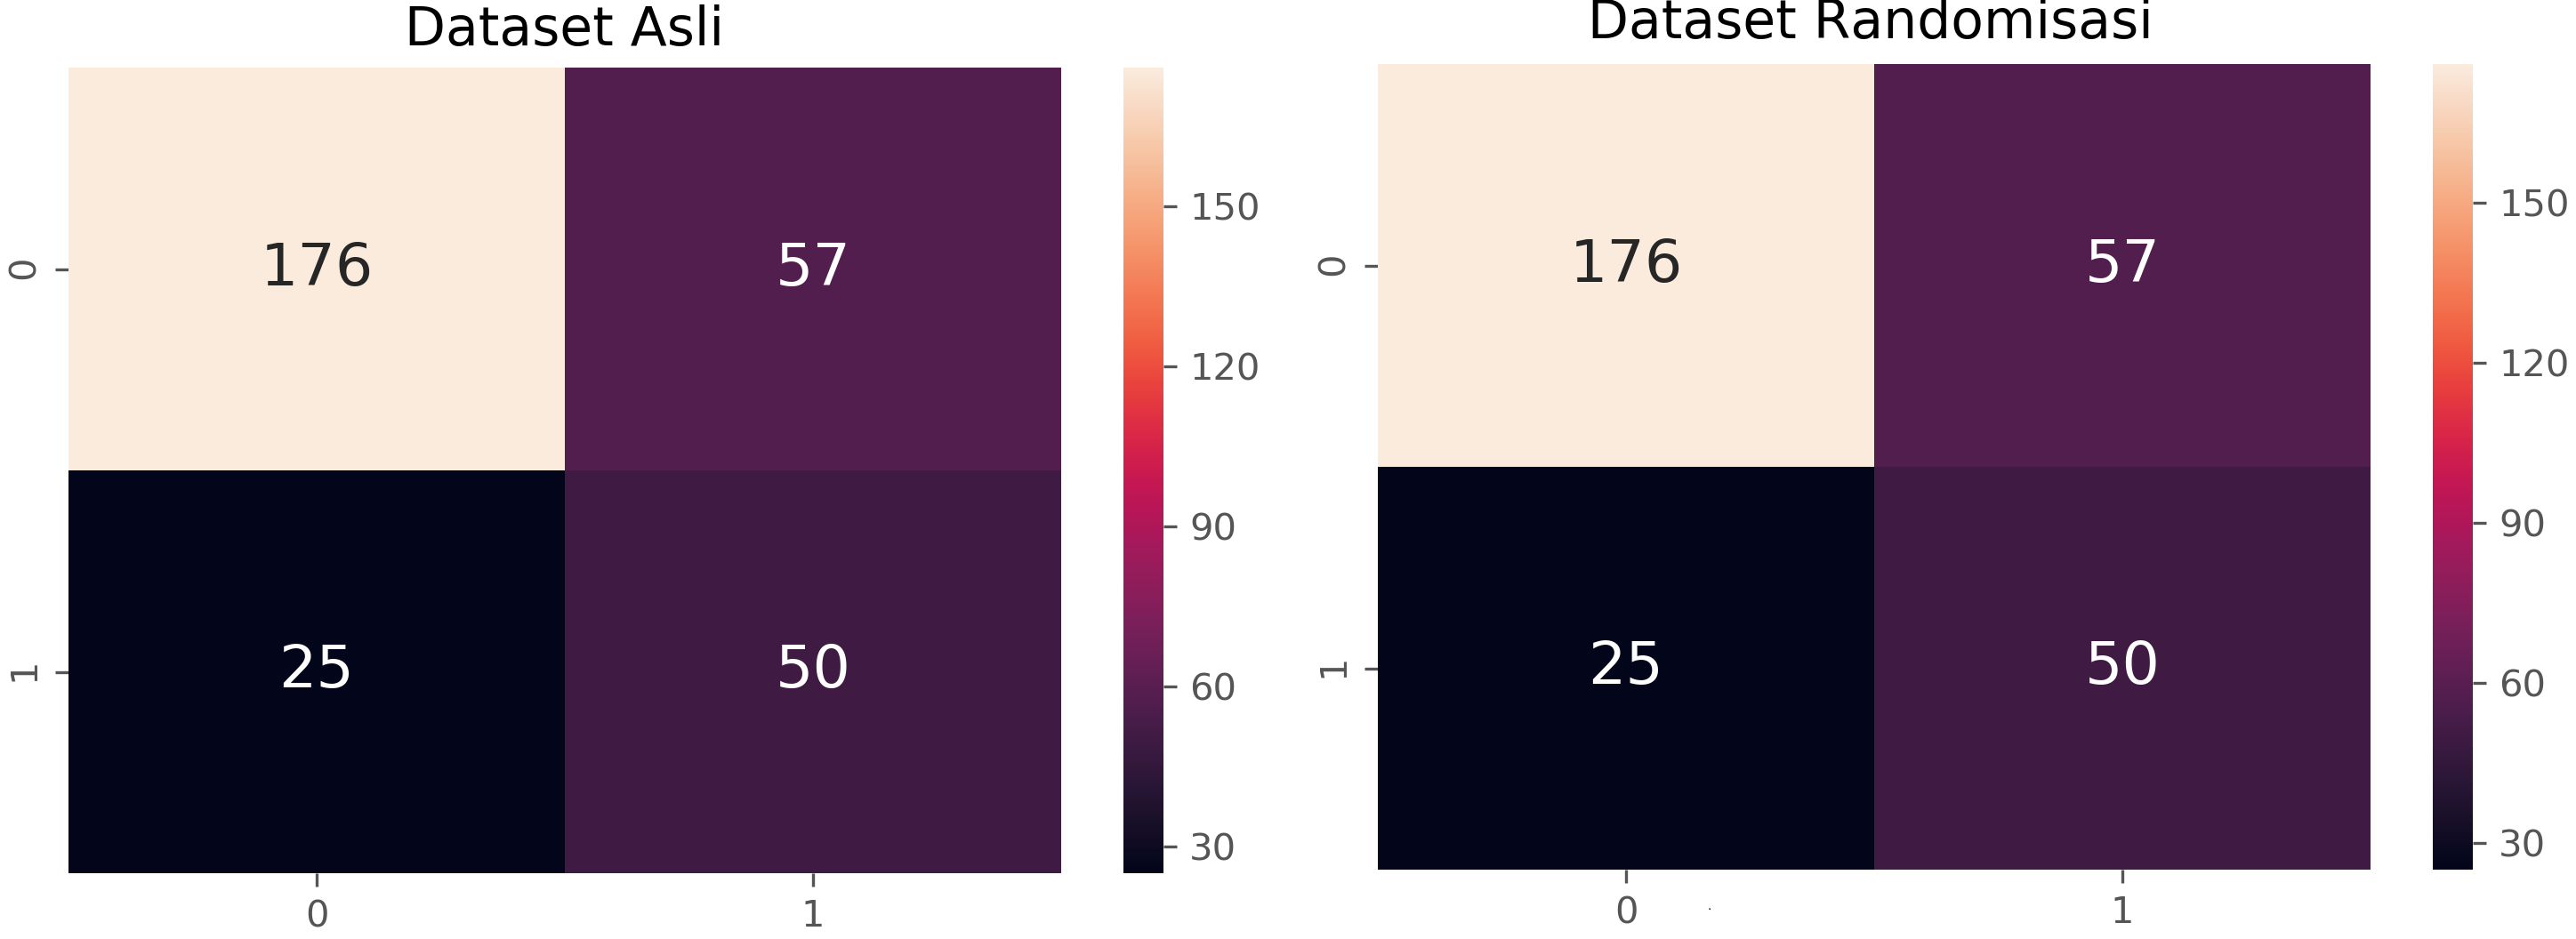
\includegraphics[scale=0.185]{confusion_diabetes}
		\caption{\textit{Confusion matrix} pada hasil prediksi \textit{test set} dataset \textit{diabetes}}
		\label{fig:confusion_diabetes}
	\end{figure}
\end{itemize}

Teknik \textit{Random Rotation Perturbation} terbukti bekerja dengan baik untuk mengacak data sehingga privasi pada data tersebut hilang tetapi data masih dapat digunakan untuk membuat model klasifikasi dengan algoritma \textit{K-nearest Neighbors} dengan hasil yang memuaskan. 

\subsubsection{\textit{Random Projection Perturbation}}
\label{sec:pengujian-klasifikasi-rpp}

Pengujian teknik \textit{Random Projection Perturbation} untuk penambangan data klasifikasi dengan algoritma \textit{K-nearest neighbors} akan dilakukan dengan dataset \textit{mobile\_sensor} yang dapat dilihat 20 baris pertamanya pada Gambar~\ref{fig:mobile_sensor_asli}. Dataset ini dirandomisasi dengan teknik \textit{Random Projection Perturbation} dan hasil randomisasi dapat dilihat pada Gambar~\ref{fig:projected_mobile_sensor}. Dengan kedua dataset tersebut, dilakukan penambangan data terhadap kedua dataset tersebut dan dihasilkan berbagai macam informasi yang dapat dibandingkan. Berikut adalah hasil pengujian dan penjelasannya.

\begin{itemize}
	\item Pada dataset \textit{mobile\_sensor}, jumlah orang yang melakukan aktivitas tertentu atau dengan kata lain distribusi label pada dataset ini dapat dilihat pada Gambar~\ref{fig:distribusi_label_mobile_sensor}. Dataset \textit{mobile\_sensor} asli dan dataset \textit{mobile\_sensor} yang telah dirandomisasi tentunya memiliki distribusi label yang sama karena label tidak dirandomisasi sehingga tidak berubah.

	\begin{figure}
		\centering
		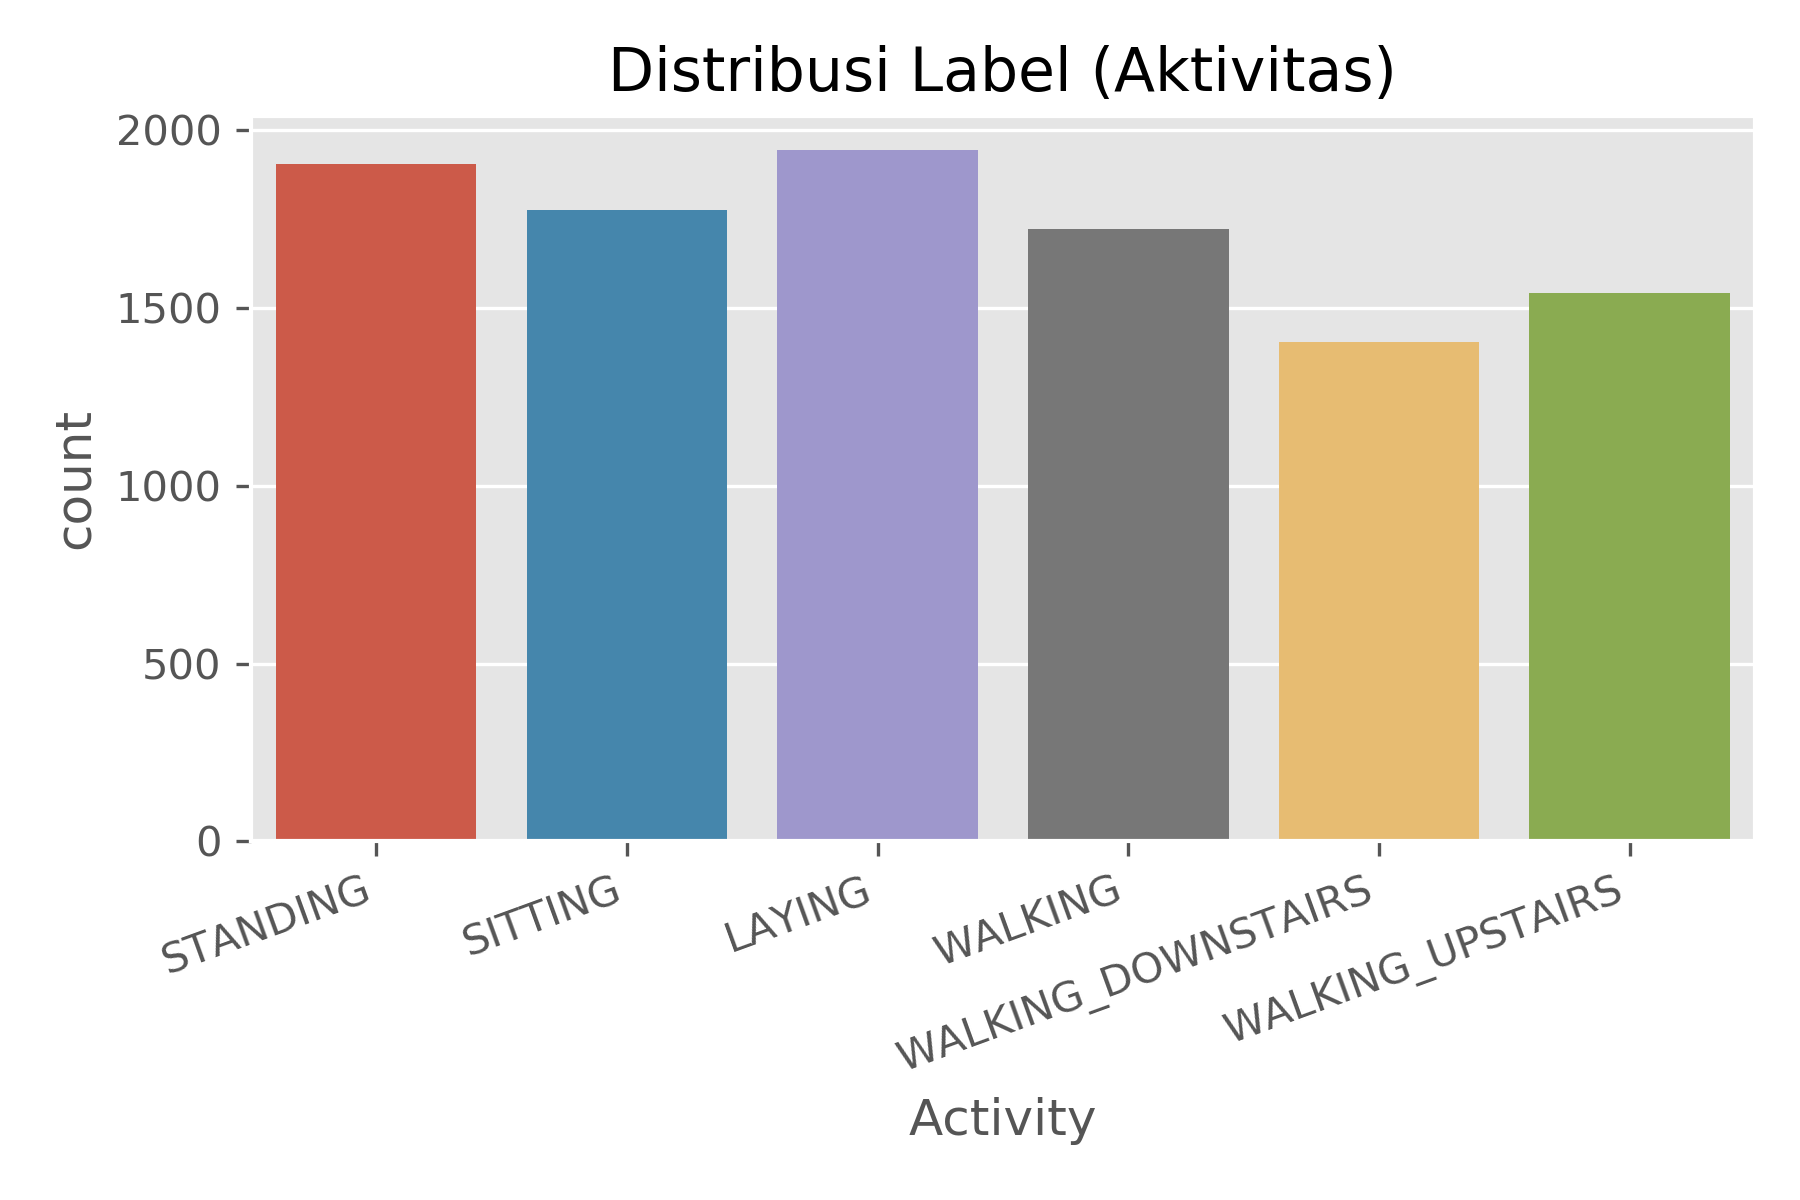
\includegraphics[scale=1]{distribusi_label_mobile_sensor}
		\caption{Histogram distribusi label dataset \textit{mobile\_sensor}}
		\label{fig:distribusi_label_mobile_sensor}
	\end{figure}
	\item Properti-properti pada dataset \textit{mobile\_sensor} asli dapat dilihat pada Tabel~\ref{table:properti-mobile-sensor-asli}. Sementara untuk dataset \textit{mobile\_sensor} yang telah dirandomisasi dapat dilihat pada Tabel~\ref{table:properti-mobile-sensor-asli}. Jika dilihat pada kedua tabel tersebut, seluruh properti pada dataset yang telah dirandomisasi mempunyai nilai yang berbeda kecuali jumlah baris (\textit{count}). Hal ini menunjukkan selain nilai pada setiap data, teknik \textit{Random Projection Perturbation} juga mengacak bermacam properti data seperti rata-rata, standar deviasi, batas bawah dan batas atas nilai pada data.

	\begin{table}
		\centering
		\caption{Properti-properti pada dataset \textit{mobile\_sensor} asli}
		\begin{tabular}{l|llll}
			\hline
			 & tBodyAcc-mean()-X & tBodyAcc-mean()-Y & angle(Y,gravityMean) & angle(Z,gravityMean)\\ \hline
			count & 10299.000000 & 10299.000000 & 10299.000000 & 10299.000000 \\
			mean & 0.274347 & -0.017743 & 0.063255 & -0.054284 \\
			std & 0.067628 & 0.037128 & 0.305468 & 0.268898 \\
			min & -1.000000 & -1.000000 & -1.000000 & -1.000000 \\
			25\% & 0.262625 & -0.024902 & 0.002151 & -0.131880 \\
			50\% & 0.277174 & -0.017162 & 0.182028 & -0.003882 \\
			75\% & 0.288354 & -0.010625 & 0.250790 & 0.102970 \\
			max & 1.000000 & 1.000000 & 1.000000 & 1.000000 \\
			\hline
		\end{tabular}
		\label{table:properti-mobile-sensor-asli}
	\end{table}
	
	\begin{table}
		\centering
		\caption{Properti-properti pada dataset \textit{mobile\_sensor} yang telah dirandomisasi}
		\begin{tabular}{l|llll}
			\hline
			& 0 & 1 & 425 & 426 \\ \hline
			count & 10299.000000 & 10299.000000 & 10299.000000 & 10299.000000 \\
			mean & 0.136942 & -0.289681 & 0.173610 & 0.353280 \\
			std & 0.528322 & 0.266849 & 0.214992 & 0.475443 \\
			min & -1.433025 & -1.206428 & -1.437424 & -0.976616 \\
			25\% & -0.340174 & -0.482918 & 0.033424 & -0.049233 \\
			50\% & 0.308314 & -0.270461 & 0.179048 & 0.322172 \\
			75\% & 0.582374 & -0.097266 & 0.325611 & 0.688616 \\
			max & 1.283867 & 0.726498 & 0.978304 & 1.786145 \\
			\hline
		\end{tabular}
		\label{table:properti-mobile-sensor-asli}
	\end{table}
	\item Teknik penambangan data \textit{K-nearest Neighbors} diterapkan menggunakan 561 fitur yang ada untuk menguji apakah dataset mempunyai akurasi model klasifikasi yang hampir sama. Pengujian tersebut didasarkan pada sifat teknik \textit{Random Projection Perturbation} yang menjamin jarak Euclidean setiap titik terjaga dengan besar \textit{error} yang ditentukan pengguna. Dataset akan dibagi dua menjadi \textit{train set} dan \textit{test set} yang masing-masing berguna untuk melatih model dan menghitung akurasi model. Akurasi akan dihitung dengan jumlah tetangga (nilai \textit{k}) dari 1 sampai 30. Implementasi kode teknik penambangan data ini diterapkan dengan bahasa pemograman Python dan dibantu oleh \textit{library} Scikit-learn.

	Pada Gambar~\ref{fig:plot_akurasi_mobile_sensor} dapat dilihat grafik akurasi model \textit{K-nearest Neighbors} dalam memprediksi label \textit{training set} dan \textit{test set} pada dataset asli dan dataset yang telah dirandomisasi. Apabila dibandingkan, kedua grafik tersebut memiliki nilai akurasi yang mirip. Walaupun begitu, teknik \textit{Random Projection Perturbation} tidak menjamin jarak Euclidean terjaga dengan sempurna maka ada sedikit perbedaan yang lumayan terlihat khususnya pada akurasi \textit{test set} dan nilai \textit{k} yang memiliki akurasi tertinggi. Tetapi perbedaan nilai akurasinya masih mirip dengan dataset asli.
	
	\begin{figure}
		\centering
		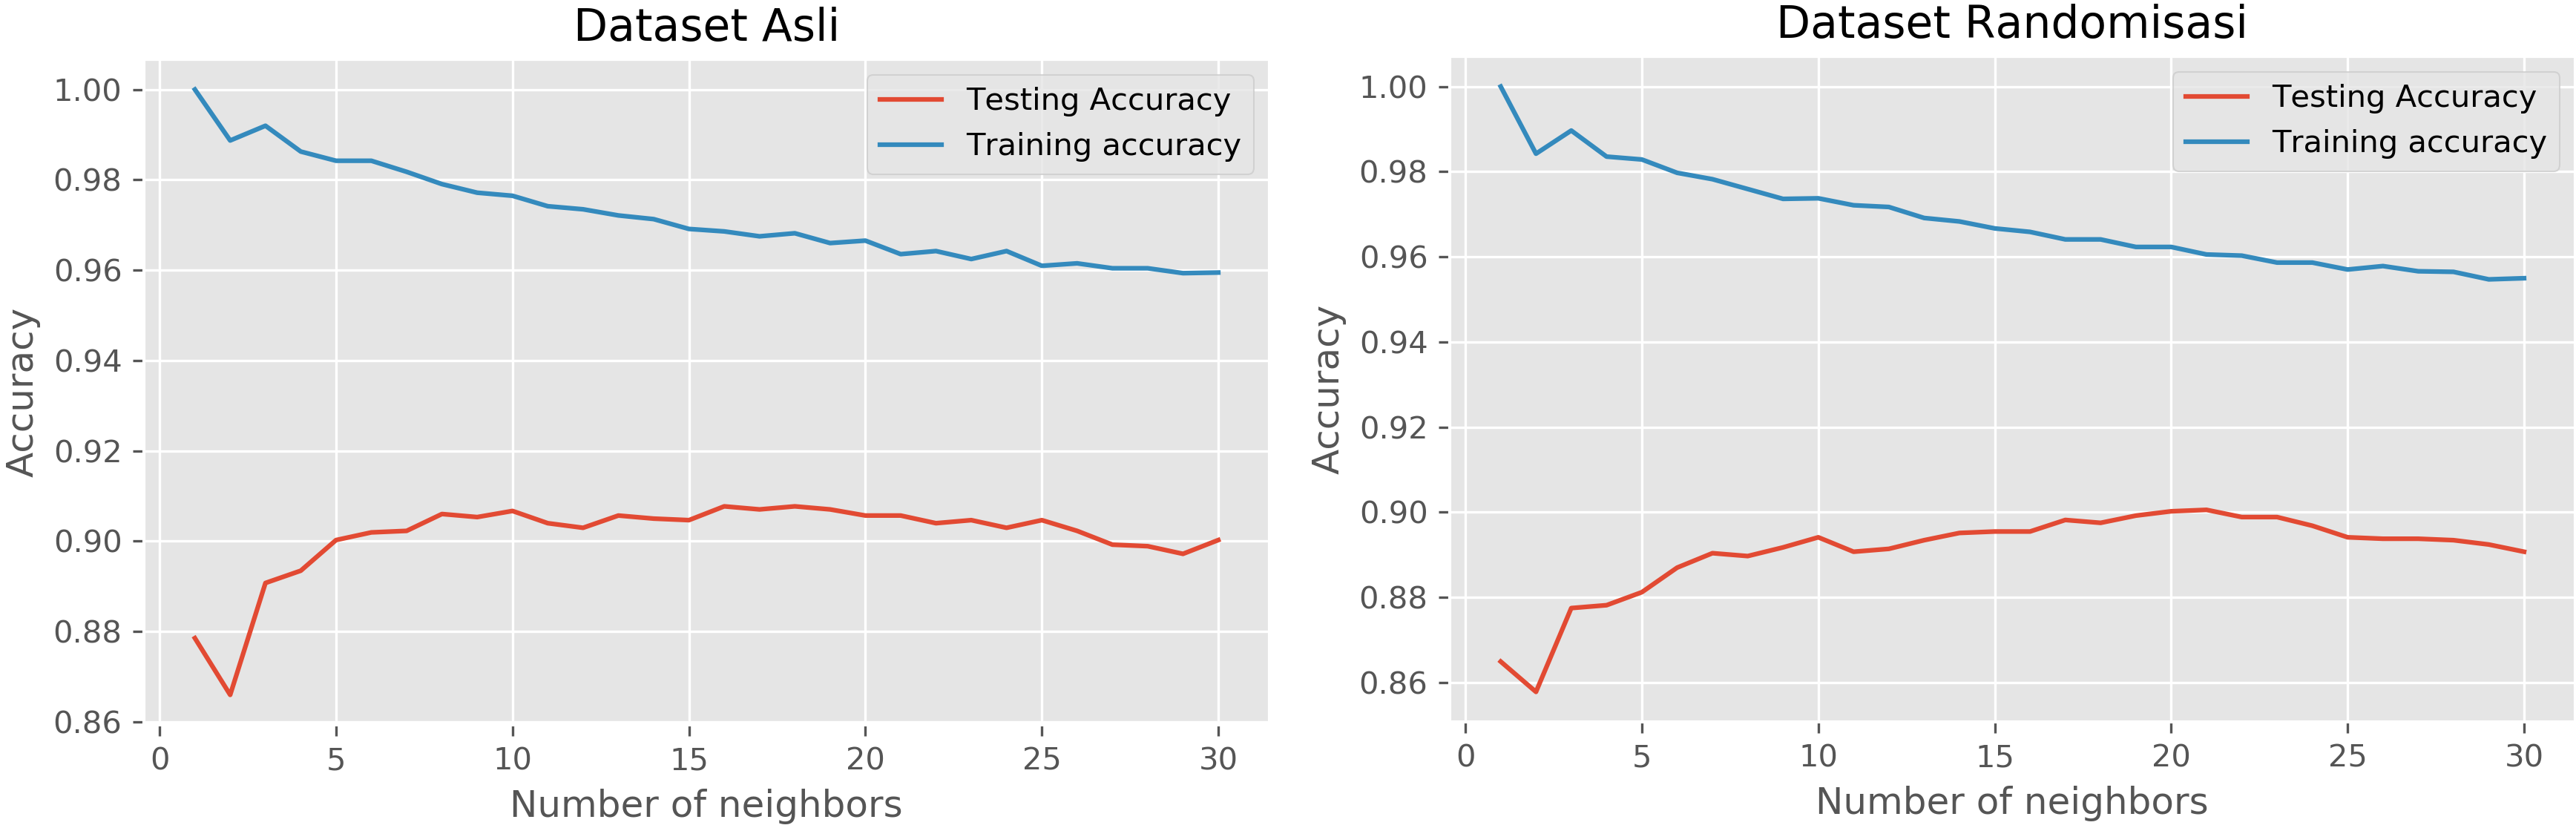
\includegraphics[scale=0.17]{plot_akurasi_mobile_sensor}
		\caption{Grafik akurasi model klasifikasi pada \textit{training set} dan \textit{test set} dataset \textit{mobile\_sensor}}
		\label{fig:plot_akurasi_mobile_sensor}
	\end{figure}
	\item Akurasi model untuk setiap nilai \textit{k} dari 11 sampai 30 pada dataset asli dan dataset yang telah dirandomisasi dapat dilihat masing-masing pada Listing~\ref{mobile_sensor_akurasi_asli} dan Listing~\ref{mobile_sensor_akurasi_randomisasi}. Dapat dilihat pada kedua listing tersebut akurasi \textit{test set} pada kedua dataset berbeda. Akurasi \textit{test set} tertinggi pada dataset asli adalah sebesar 0.9077027485578555 dengan nilai \textit{k} sebesar 16. Sementara pada dataset yang telah dirandomisasi, akurasi \textit{test set} tertingginya adalah sebesar 0.9005768578215134 dengan nilai \textit{k} sebesar 21. Jika dihitung perbedaan akurasinya adalah sebesar 0.0071258907363421 yang mana relatif kecil tetapi ada perbedaan pada nilai \textit{k} yang memiliki akurasi tertinggi. Dengan perbedaan akurasi yang relatif kecil dan dataset yang telah dirandomisasi teracak dengan baik maka dapat disimpulkan bahwa teknik \textit{Random Projection Perturbation} menjaga jarak Euclidean dengan baik dan \textit{error}-nya terkontrol sesuai yang pengguna inginkan. Oleh karena itu, model \textit{K-nearest Neighbors} yang terbuat memiliki hasil yang sangat mirip.

	\noindent\begin{minipage}{.44\textwidth}
	\begin{lstlisting}[caption=Akurasi Dataset Asli,frame=tlrb, label=mobile_sensor_akurasi_asli]{Name}
Akurasi setiap K pada 
training set dataset asli: 
11: 0.9741566920565833
12: 0.9734766050054406
13: 0.9721164309031556
14: 0.9713003264417845
15: 0.9691240478781284
16: 0.9685799782372143
17: 0.9674918389553863
18: 0.9681719260065288
19: 0.9659956474428727
20: 0.9665397170837867
21: 0.9635473340587595
22: 0.9642274211099021
23: 0.9624591947769314
24: 0.9642274211099021
25: 0.9609630032644179
26: 0.9615070729053319
27: 0.9604189336235038
28: 0.9604189336235038
29: 0.9593307943416758
30: 0.9594668117519043

Akurasi setiap K pada 
test set dataset asli: 
11: 0.9039701391245334
12: 0.9029521547336274
13: 0.9056667797760435
14: 0.9049881235154394
15: 0.9046487953851374
16: 0.9077027485578555
17: 0.9070240922972514
18: 0.9077027485578555
19: 0.9070240922972514
20: 0.9056667797760435
21: 0.9056667797760435
22: 0.9039701391245334
23: 0.9046487953851374
24: 0.9029521547336274
25: 0.9046487953851374
26: 0.9022734984730234
27: 0.8992195453003053
28: 0.8988802171700034
29: 0.8971835765184933
30: 0.9002375296912114
	\end{lstlisting}
	\end{minipage}\hfill
	\begin{minipage}{.46\textwidth}
	\begin{lstlisting}[caption=Akurasi Dataset Randomisasi,frame=tlrb, label=mobile_sensor_akurasi_randomisasi]{Name}
Akurasi setiap K pada training 
set dataset randomisasi: 
11: 0.9721164309031556
12: 0.9717083786724701
13: 0.9691240478781284
14: 0.9683079434167573
15: 0.9666757344940152
16: 0.9658596300326442
17: 0.9640914036996736
18: 0.9640914036996736
19: 0.9623231773667029
20: 0.9623231773667029
21: 0.9605549510337323
22: 0.9602829162132753
23: 0.9586507072905331
24: 0.9586507072905331
25: 0.9570184983677911
26: 0.9578346028291621
27: 0.9566104461371056
28: 0.956474428726877
29: 0.9547062023939065
30: 0.9549782372143635

Akurasi setiap K pada test 
set dataset randomisasi: 
11: 0.8907363420427553
12: 0.8914149983033594
13: 0.8934509670851714
14: 0.8951476077366813
15: 0.8954869358669834
16: 0.8954869358669834
17: 0.8982015609093994
18: 0.8975229046487954
19: 0.8992195453003053
20: 0.9002375296912114
21: 0.9005768578215134
22: 0.8988802171700034
23: 0.8988802171700034
24: 0.8968442483881914
25: 0.8941296233457754
26: 0.8937902952154734
27: 0.8937902952154734
28: 0.8934509670851714
29: 0.8924329826942654
30: 0.8907363420427553
	\end{lstlisting}
	\end{minipage}
	\item Waktu eksekusi yang dibutuhkan untuk melatih model klasifikasi dengan nilai \textit{k} sebesar 16 memakai dataset asli adalah sebesar 0.2872335910797119 detik dan waktu yang dibutuhkan untuk memprediksi \textit{test set} sebesar 17.754546642303467 detik. Sementara untuk dataset yang telah dirandomisasi membutuhkan waktu eksekusi untuk melatih model klasifikasi dengan nilai \textit{k} sebesar 21 adalah 0.5630350112915039 detik detik dan waktu yang dibutuhkan untuk melakukan prediksi adalah sebesar 12.86760687828064 detik. Pada dataset yang telah dirandomisasi waktu prediksi lebih cepat dikarenakan fitur-fitur yang ada pun lebih sedikit daripada dataset asli. Hal ini menunjukkan ada pengaruh yang signifikan terhadap durasi waktu eksekusi untuk melatih model dan memprediksi dengan dataset asli dan dataset yang telah dirandomisasi.
	\item Pada Gambar~\ref{fig:confusion_matrix_mobile_sensor} dapat dilihat \textit{confusion matrix} pada model klasifikasi dengan nilai \textit{k} sebesar 16 memakai \textit{test set} pada dataset asli dan nilai \textit{k} sebesar 21 memakai dataset yang telah dirandomisasi. Apabila dibandingkan antar keduanya, \textit{confusion matrix} yang ada memiliki nilai yang sangat mirip. Oleh karena itu, akurasi modelnya juga mempunyai nilai yang sangat mirip. Hal ini juga menguatkan kesimpulan bahwa teknik \textit{Random Projection Perturbation} menjaga jarak Euclidean dengan baik dan \textit{error}-nya terkontrol sesuai yang pengguna inginkan.

	\begin{figure}
		\centering
		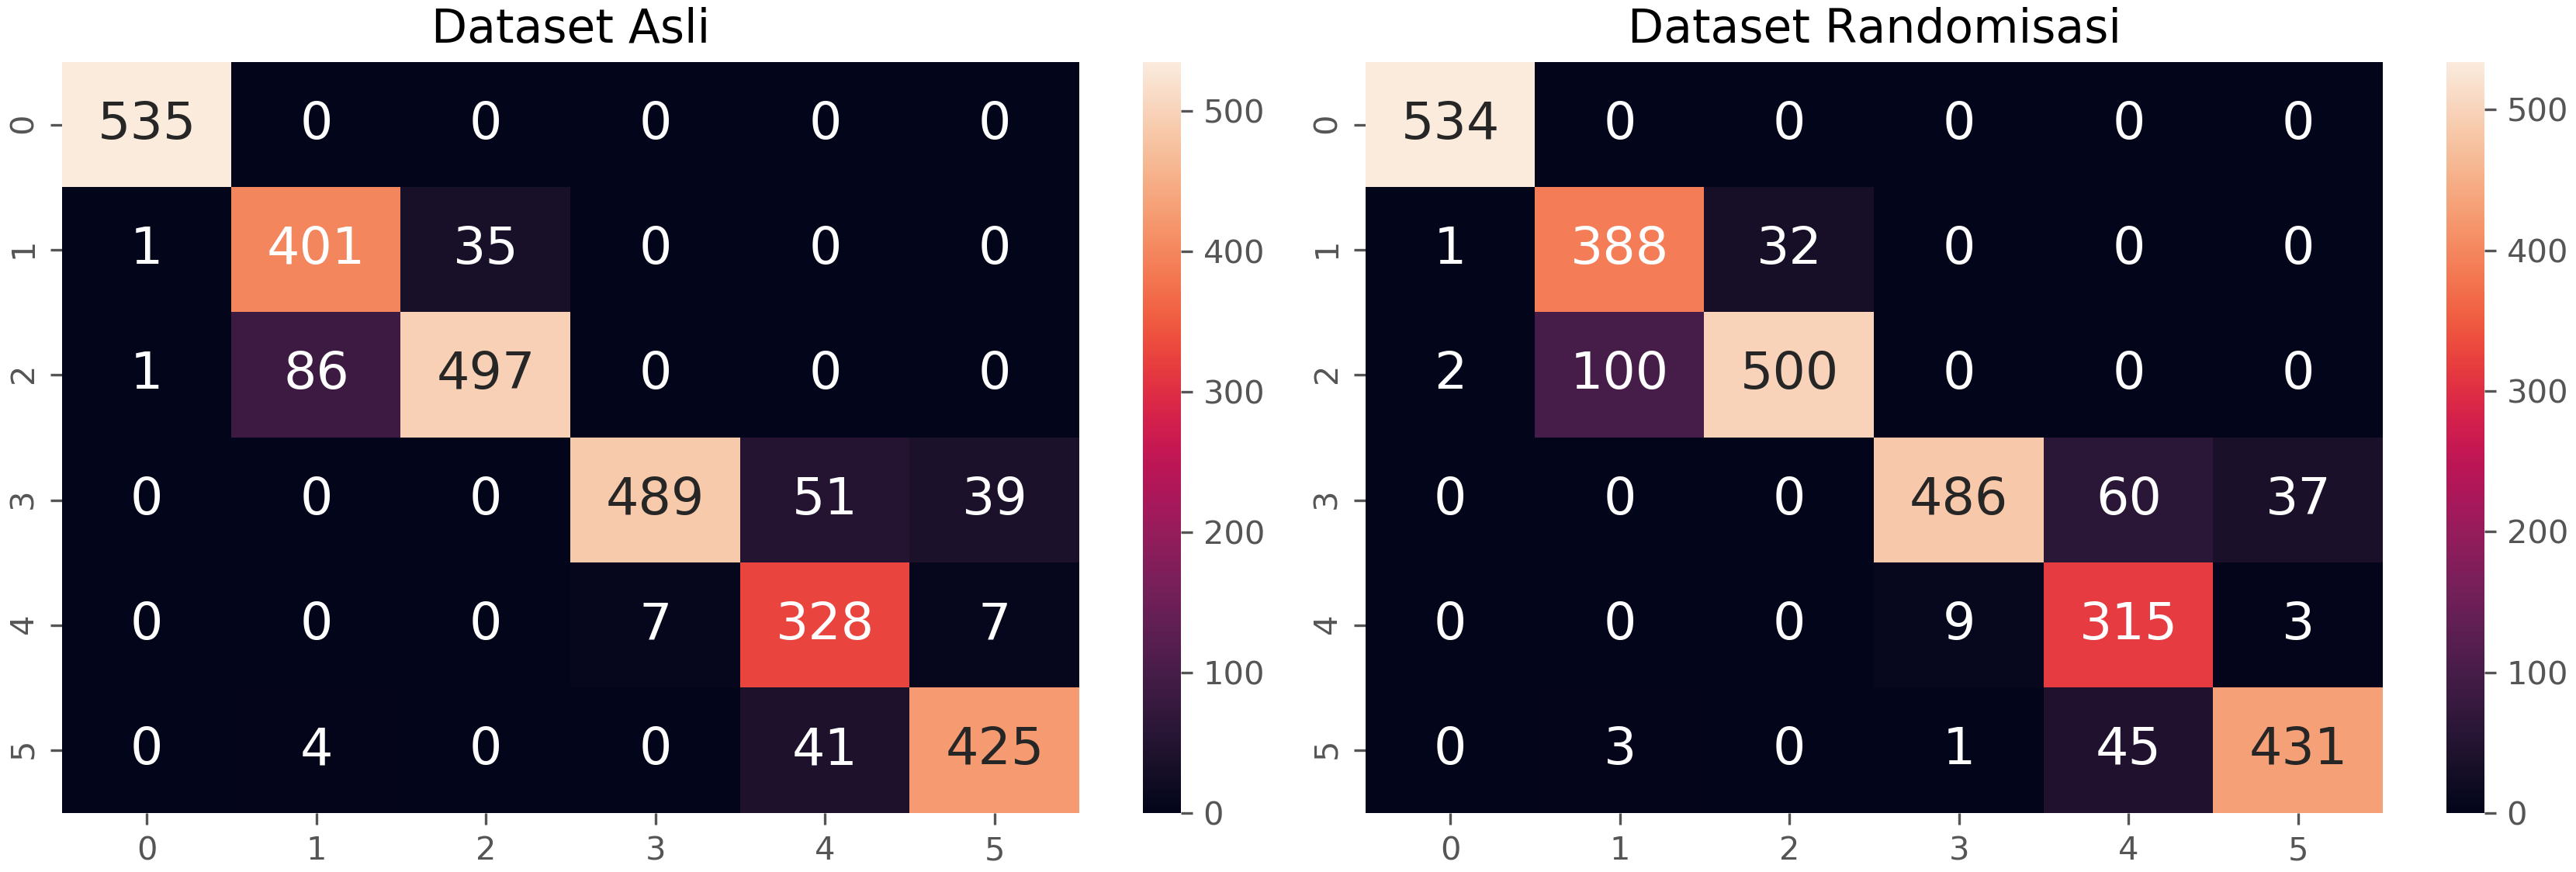
\includegraphics[scale=0.185]{confusion_matrix_mobile_sensor}
		\caption{\textit{Confusion matrix} pada hasil prediksi \textit{test set} dataset \textit{mobile\_sensor}}
		\label{fig:confusion_matrix_mobile_sensor}
	\end{figure}
\end{itemize}

Teknik \textit{Random Projection Perturbation} terbukti bekerja dengan baik untuk mengacak data yang ukurannya cukup besar sehingga privasi pada data tersebut hilang tetapi data masih dapat digunakan untuk membuat model klasifikasi dengan algoritma \textit{K-nearest Neighbors} dengan hasil yang memuaskan.

\subsection{Penambangan Data \textit{Clustering}}
\label{sec:pengujian-clustering}

Pengujian dengan penambangan data \textit{clustering} akan berpusat pada pembuatan model \textit{clustering} dengan dataset asli dan dataset yang telah dirandomisasi dan membandingkan kualitas model tersebut. Teknik penambangan data \textit{clustering} yang digunakan adalah \textit{K-means}. Berikut hasil pengujian eksperimental yang telah dilakukan.

\subsubsection{\textit{Random Rotation Perturbation}}
\label{sec:pengujian-clustering-rrp}

Pengujian teknik \textit{Random Rotation Perturbation} untuk penambangan data \textit{clustering} dengan algoritma \textit{K-means} akan dilakukan dengan dataset \textit{mall\_customers} yang dapat dilihat 20 baris pertamanya pada Gambar~\ref{fig:mall_customers_asli}. Dataset ini dirandomisasi dengan teknik \textit{Random Rotation Perturbation} dan hasil randomisasi dapat dilihat pada Gambar~\ref{fig:rotated_mall_customers}. Dengan kedua dataset tersebut, dilakukan penambangan data terhadap kedua dataset tersebut dan dihasilkan berbagai macam informasi yang dapat dibandingkan. Berikut adalah hasil pengujian dan penjelasannya.

\begin{itemize}
	\item Properti-properti pada dataset \textit{mall\_customers} asli dapat dilihat pada Tabel~\ref{table:properti-mall-customers-asli}. Sementara untuk dataset \textit{diabetes} yang telah dirandomisasi dapat dilihat pada Tabel~\ref{table:properti-mall-customers-randomisasi}. Jika dilihat pada kedua tabel tersebut, seluruh properti pada dataset yang telah dirandomisasi mempunyai nilai yang berbeda kecuali jumlah baris (\textit{count}). Hal ini menunjukkan selain nilai pada setiap data, teknik \textit{Random Rotation Perturbation} juga mengacak bermacam properti data seperti rata-rata, standar deviasi, batas bawah dan batas atas nilai pada data.


	\begin{table}
		\centering
		\caption{Properti-properti pada dataset \textit{mall\_customers} asli}
		\begin{tabular}{l|lll}
			\hline
			& Age & Annual Income (k\$) & Spending Score (1-100) \\ 
	 count& 200.000000 & 200.000000 & 200.000000 \\
	 mean & 38.850000 & 60.560000 & 50.200000 \\
	 std & 13.969007 & 26.264721 & 25.823522 \\
	 min & 18.000000 & 15.000000 & 1.000000 \\
	 25\% & 28.750000 & 41.500000 & 34.750000 \\
	 50\% & 36.000000 & 61.500000 & 50.000000 \\
	 75\% & 49.000000 & 78.000000 & 73.000000 \\
	 max & 70.000000 & 137.000000 & 99.000000 \\
			\hline
		\end{tabular}
		\label{table:properti-mall-customers-asli}
	\end{table}
	
	\begin{table}
		\centering
		\caption{Properti-properti pada dataset \textit{mall\_customers} yang telah dirandomisasi}
		\begin{tabular}{l|lll}
			\hline
			& Age & Annual Income (k\$) & Spending Score (1-100) \\ 
	 count& 200.000000 & 200.000000 & 200.000000 \\
	 mean & 59.295607 & -72.113582 & -192.830387 \\
	 std & 24.832342 & 22.891719 & 20.276760 \\
	 min & 3.246983 & -113.632925 & -246.309601 \\
	 25\% & 43.595492 & -92.541715 & -206.989917 \\
	 50\% & 56.497882 & -68.628508 & -190.676923 \\
	 75\% & 73.795114 & -53.968669 & -180.098255 \\
	 max & 140.690958 & -17.887145 & -131.806548 \\
			\hline
		\end{tabular}
		\label{table:properti-mall-customers-randomisasi}
	\end{table}
	\item Pada Gambar~\ref{fig:pairplot_mall_customers} terdapat \textit{scatter plot} antara satu fitur dengan fitur lainnya pada dataset asli dan dataset yang telah dirandomisasi. Dapat terlihat pada kedua \textit{scatter plot} tersebut, lokasi pada titik-titik pada seluruh scatter plot berbeda. Hal ini menunjukkan teknik \textit{Random Rotation Perturbation} berhasil mengacak dengan baik setiap nilai yang ada dengan rotasi sehingga visualisasi seperti ini akan terlihat acak karena dataset dirotasi pada dimensi yang lebih besar.

	\begin{figure}
		\centering
		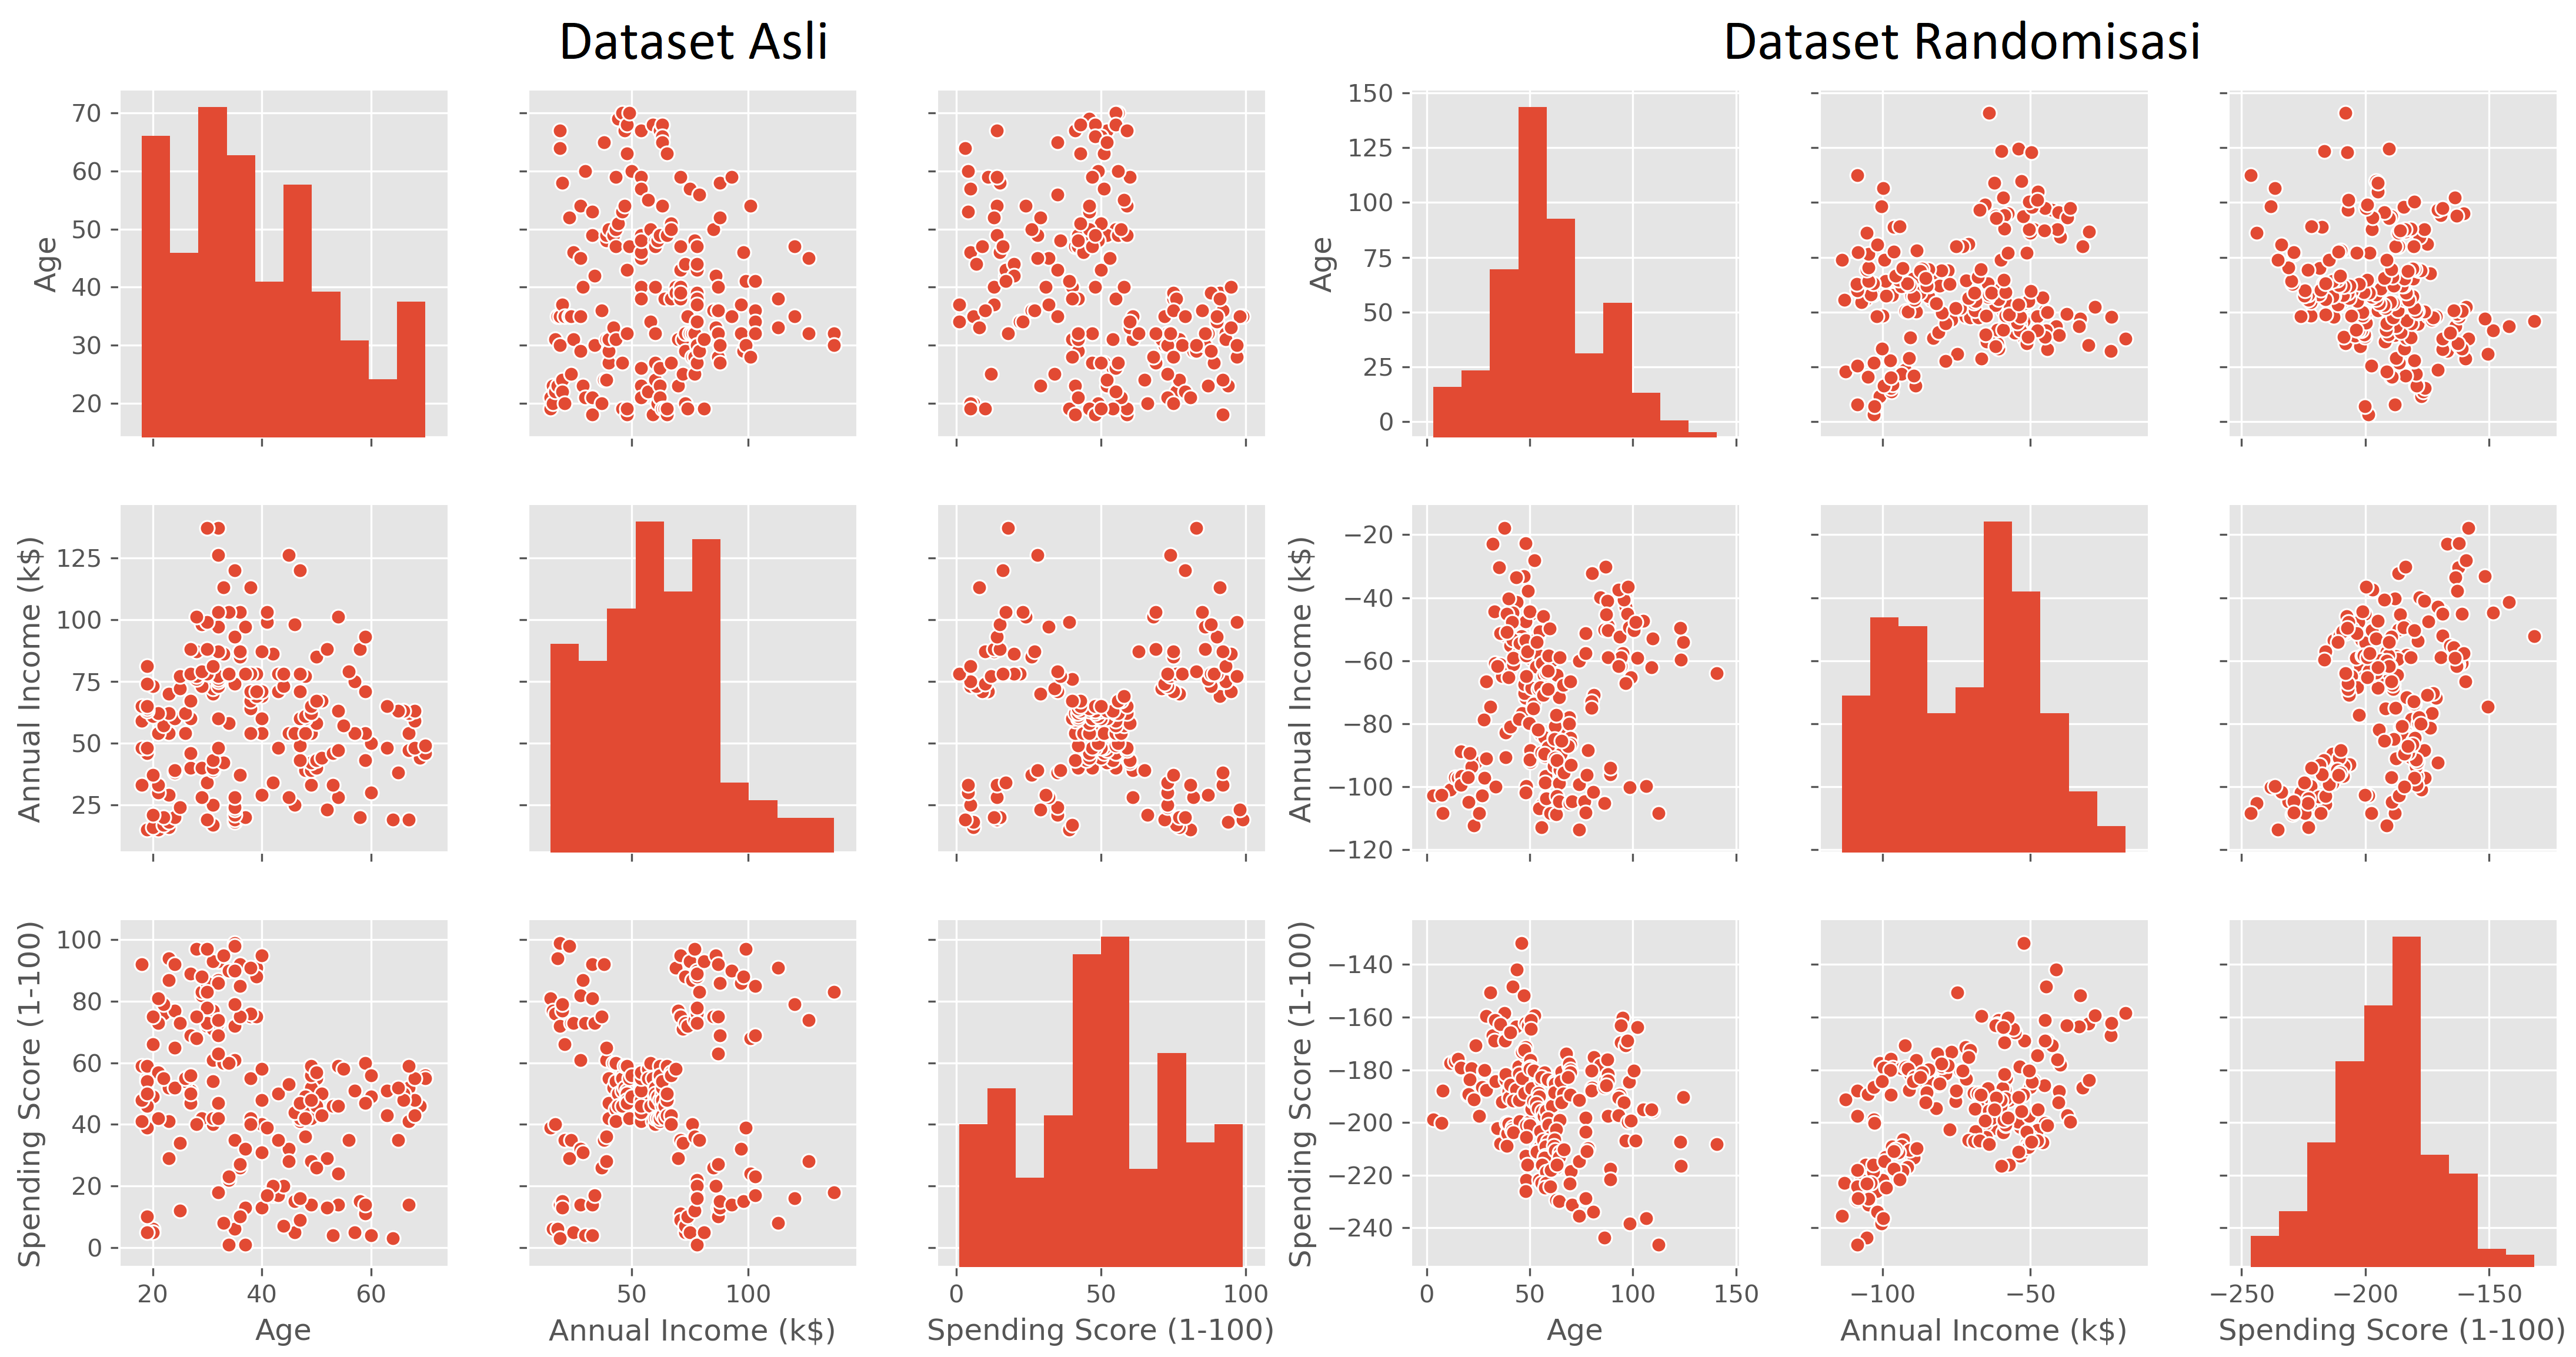
\includegraphics[scale=0.13]{pairplot_mall_customers}
		\caption{\textit{Scatter plot} antara seluruh fitur pada dataset \textit{mall\_customers} yang asli}
		\label{fig:pairplot_mall_customers}
	\end{figure}
	
	\item Pada Gambar~\ref{fig:heatmap_mall_customers} dapat dilihat korelasi antara satu fitur dengan fitur lainnya pada dataset asli dan dataset yang telah dirandomisasi. Apabila dibandingkan korelasi antar fitur pada dataset randomisasi sangat berbeda dengan dataset asli, bahkan tidak terlihat ada indikasi kesamaan atau ada properti pada dataset asli yang sama dengan dataset randomisasi. Hal ini menunjukkan teknik \textit{Random Rotation Perturbation} mengacak setiap nilai pada data tanpa menjaga properti lain selain jarak Euclidean.

	\begin{figure}
		\centering
		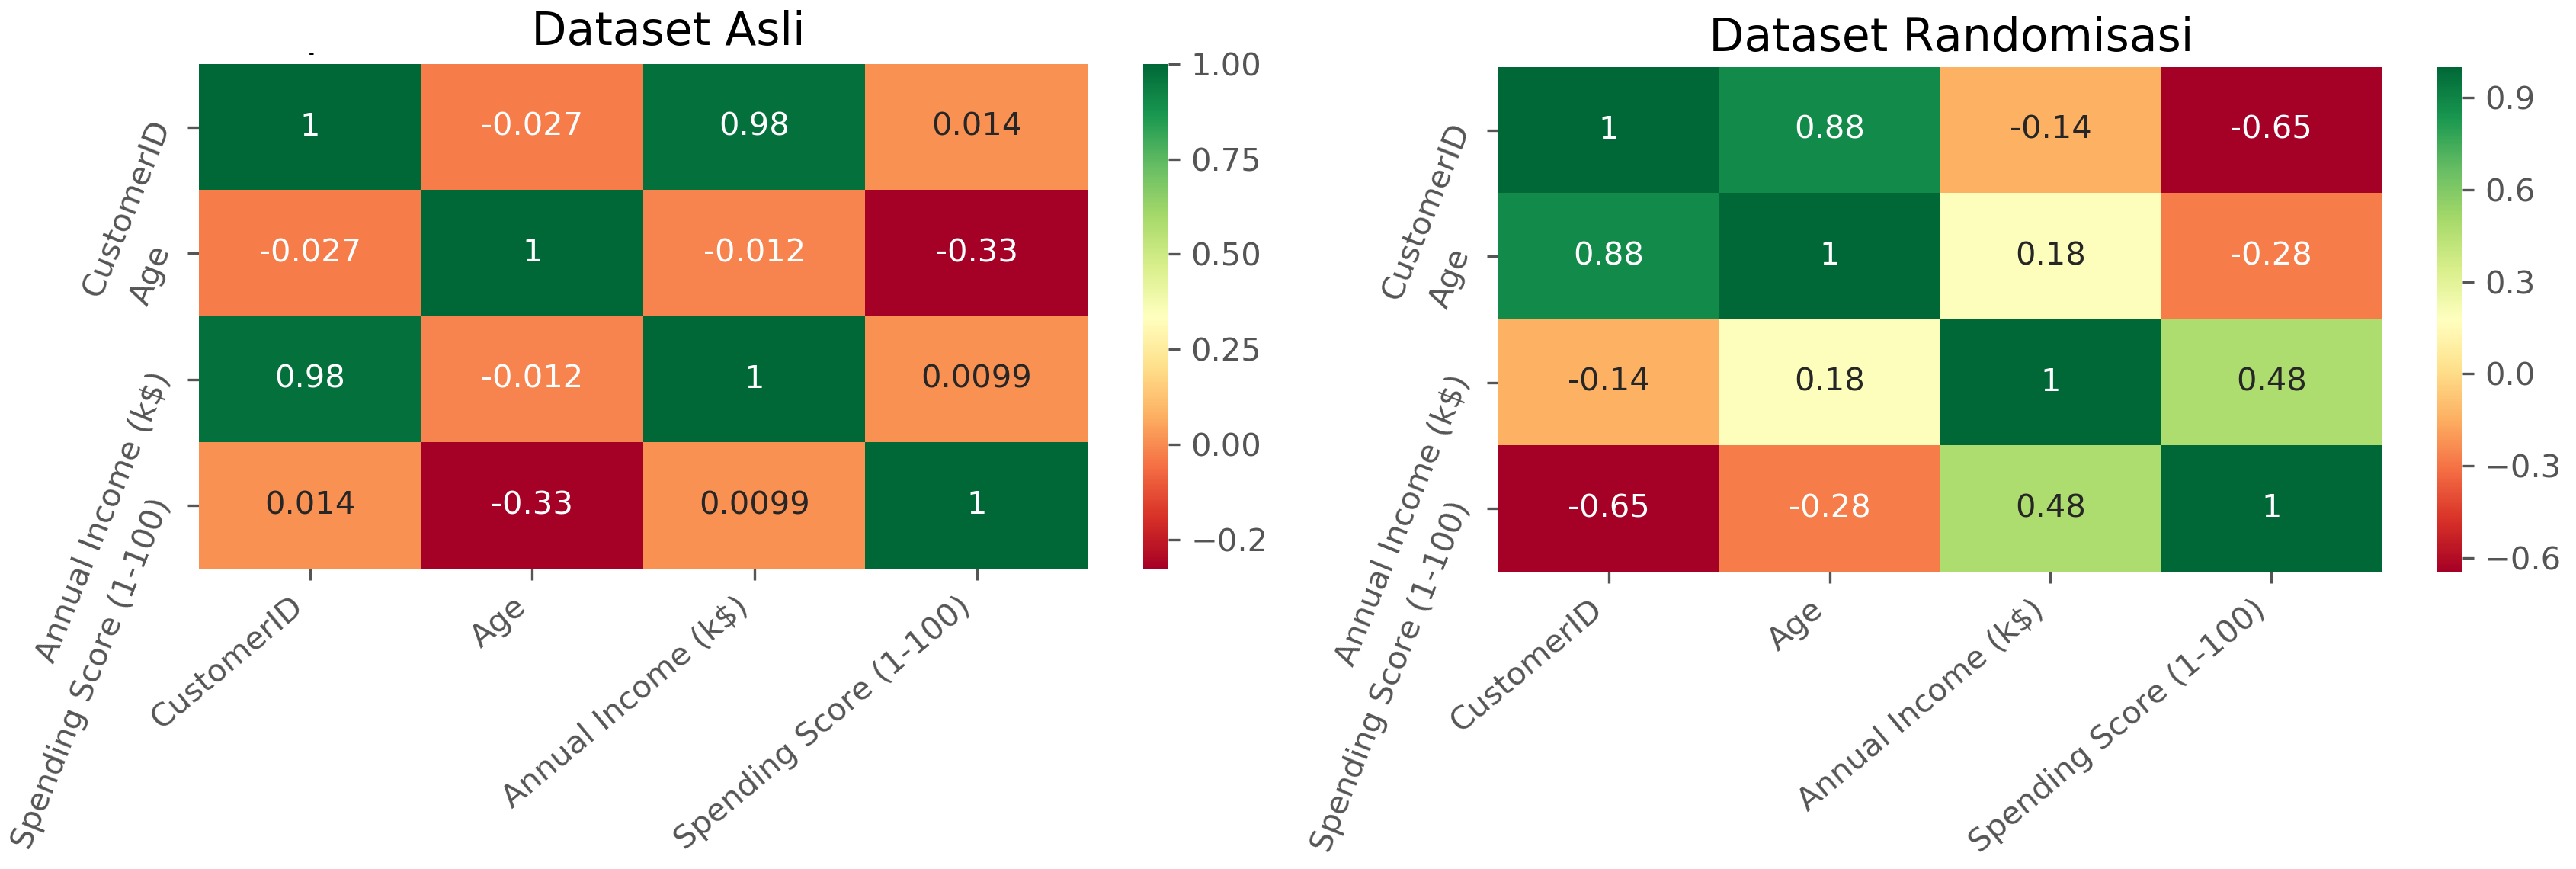
\includegraphics[scale=0.18]{heatmap_mall_customers}
		\caption{\textit{Heatmap} korelasi antar fitur pada dataset \textit{mall\_customers}}
		\label{fig:heatmap_mall_customers}
	\end{figure}

	\item Dalam menentukan jumlah \textit{cluster} atau nilai \textit{k} yang terbaik untuk membuat model \textit{clustering} dengan algoritma \textit{k-means} perlu ada metode untuk menentukan nilai tersebut. Metode Elbow menjadi salah satu metode yang digunakan untuk menentukan nilai \textit{k} yang terbaik untuk dipakai. Pada Gambar~\ref{fig:elbow_mall_customers} terdapat grafik \textit{SSE} untuk menggunakan metode Elbow pada dataset asli dan dataset yang telah dirandomisasi. Terlihat nilai \textit{k} sebesar 5, 6, dan 7 adalah kandidat yang terbaik untuk menjadi nilai \textit{k} yang dipakai pada dataset asli maupun dataset randomisasi. Pada kedua dataset tersebut grafik \textit{SSE}-nya terlihat sama persis dikarenakan teknik \textit{Random Rotation Perturbation} menjaga jarak Euclidean dengan sempurna. Dalam menentukan nilai \textit{k} yang terbaik antara ketiga nilai tersebut, \textit{Sillhoutte Score} dapat digunakan untuk metode alternatif untuk menentukan nilai \textit{k} yang terbaik.

	\begin{figure}
		\centering
		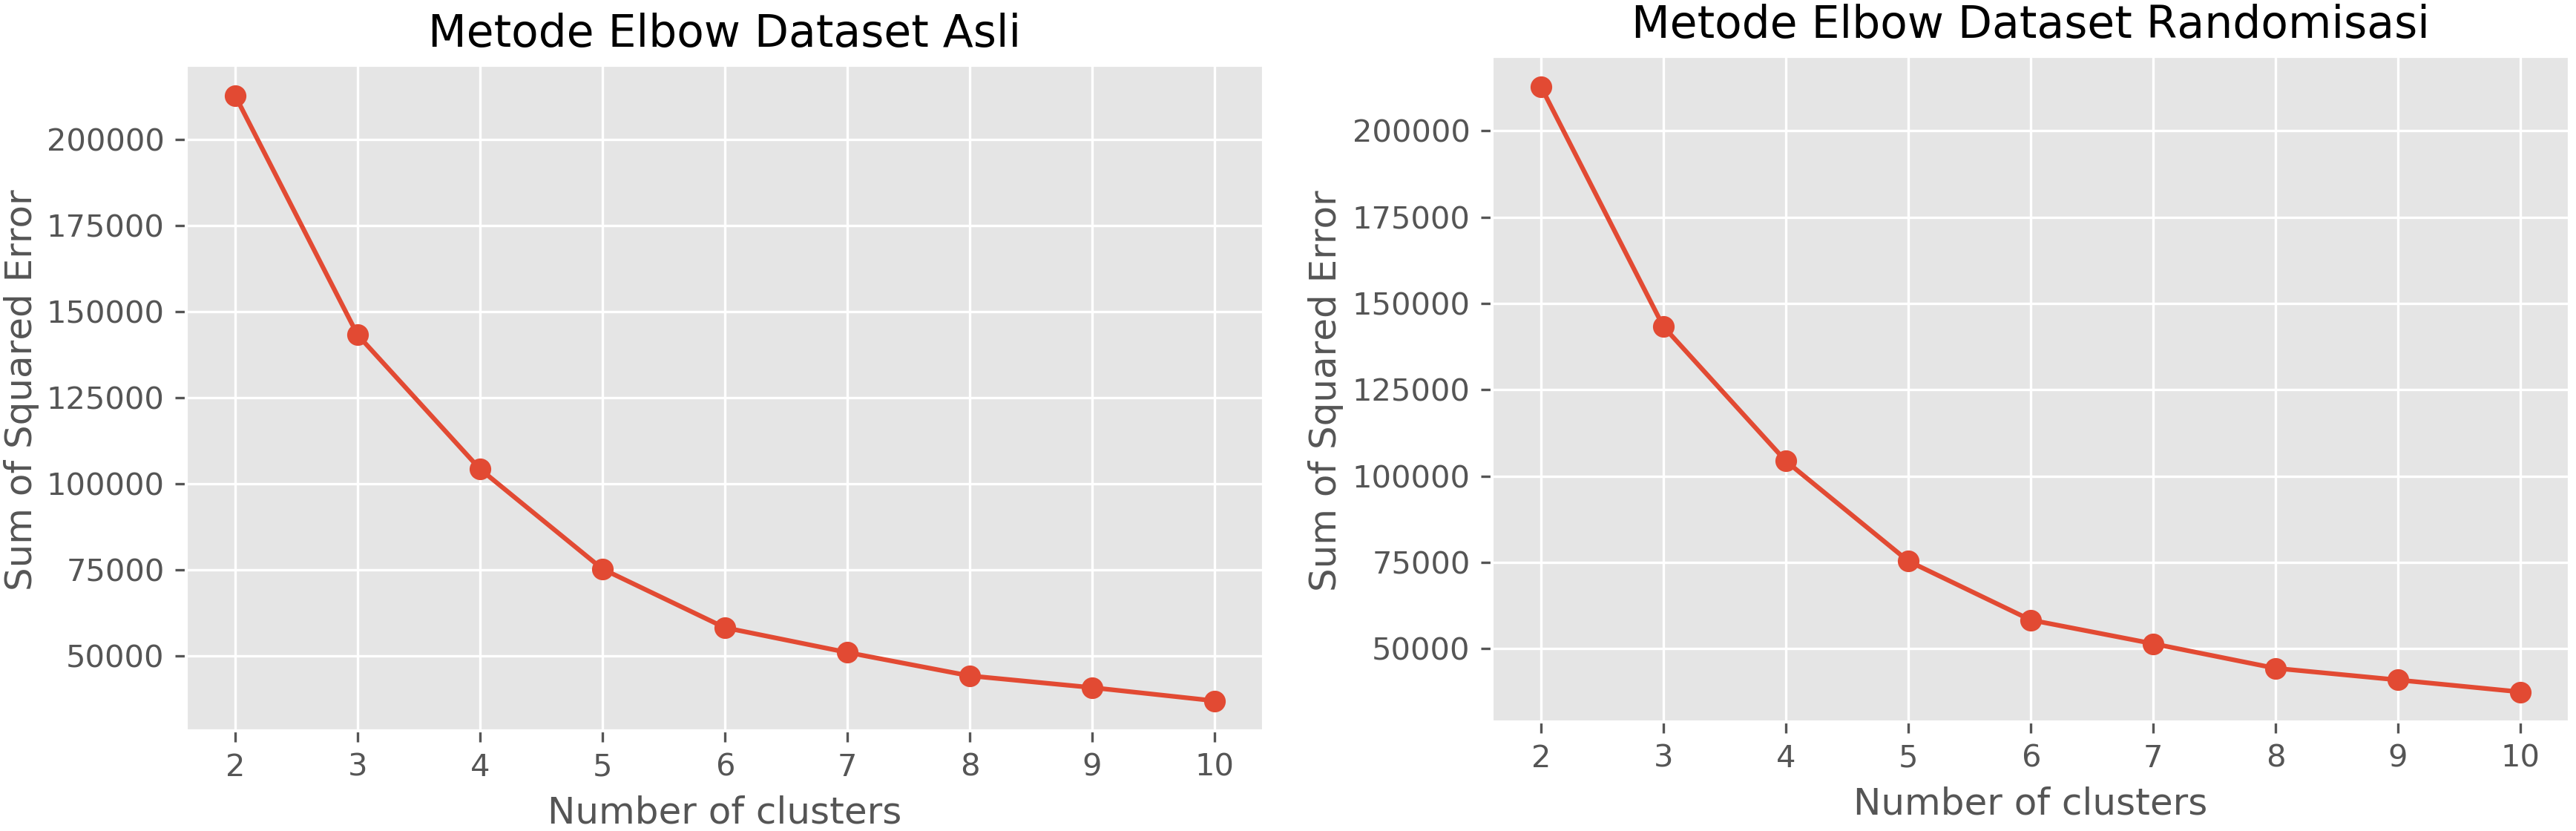
\includegraphics[scale=0.17]{elbow_mall_customers}
		\caption{Grafik \textit{SSE} untuk menggunakan metode Elbow untuk mencari nilai \textit{k} terbaik}
		\label{fig:elbow_mall_customers}
	\end{figure}

	\item Pada Gambar~\ref{fig:siluet_mall_customers} terdapat grafik \textit{Sillhoutte Score} dari dataset \textit{mall\_customers} asli dan yang telah dirandomisasi. Dapat terlihat kedua grafik \textit{Sillhoutte Score} terlihat sama persis dan dapat dilihat nilai-nilai pada setiap \textit{k} tersebut di Listing~\ref{mall_customers_siluet_asli} dan Listing~\ref{mall_customers_siluet_randomisasi} ada sedikit perbedaan yang tidak terlalu signifikan. Hal ini mungkin dikarenakan oleh nilai pada setiap data yang berbeda dan mempengaruhi sedikit algoritma pada \textit{Sillhoutte Score}. Dapat terlihat \textit{Sillhoutte Score} pada nilai \textit{k} 6 adalah nilai paling besar yaitu 0.4523443947724053 pada dataset asli dan 0.4523443947780976 pada dataset yang telah dirandomisasi. Hal ini menunjukkan teknik \textit{Random Rotation Perturbation} tidak mempengaruhi secara signifikan nilai \textit{Sillhoutte Score} pada setiap \textit{k}.

	\begin{figure}
		\centering
		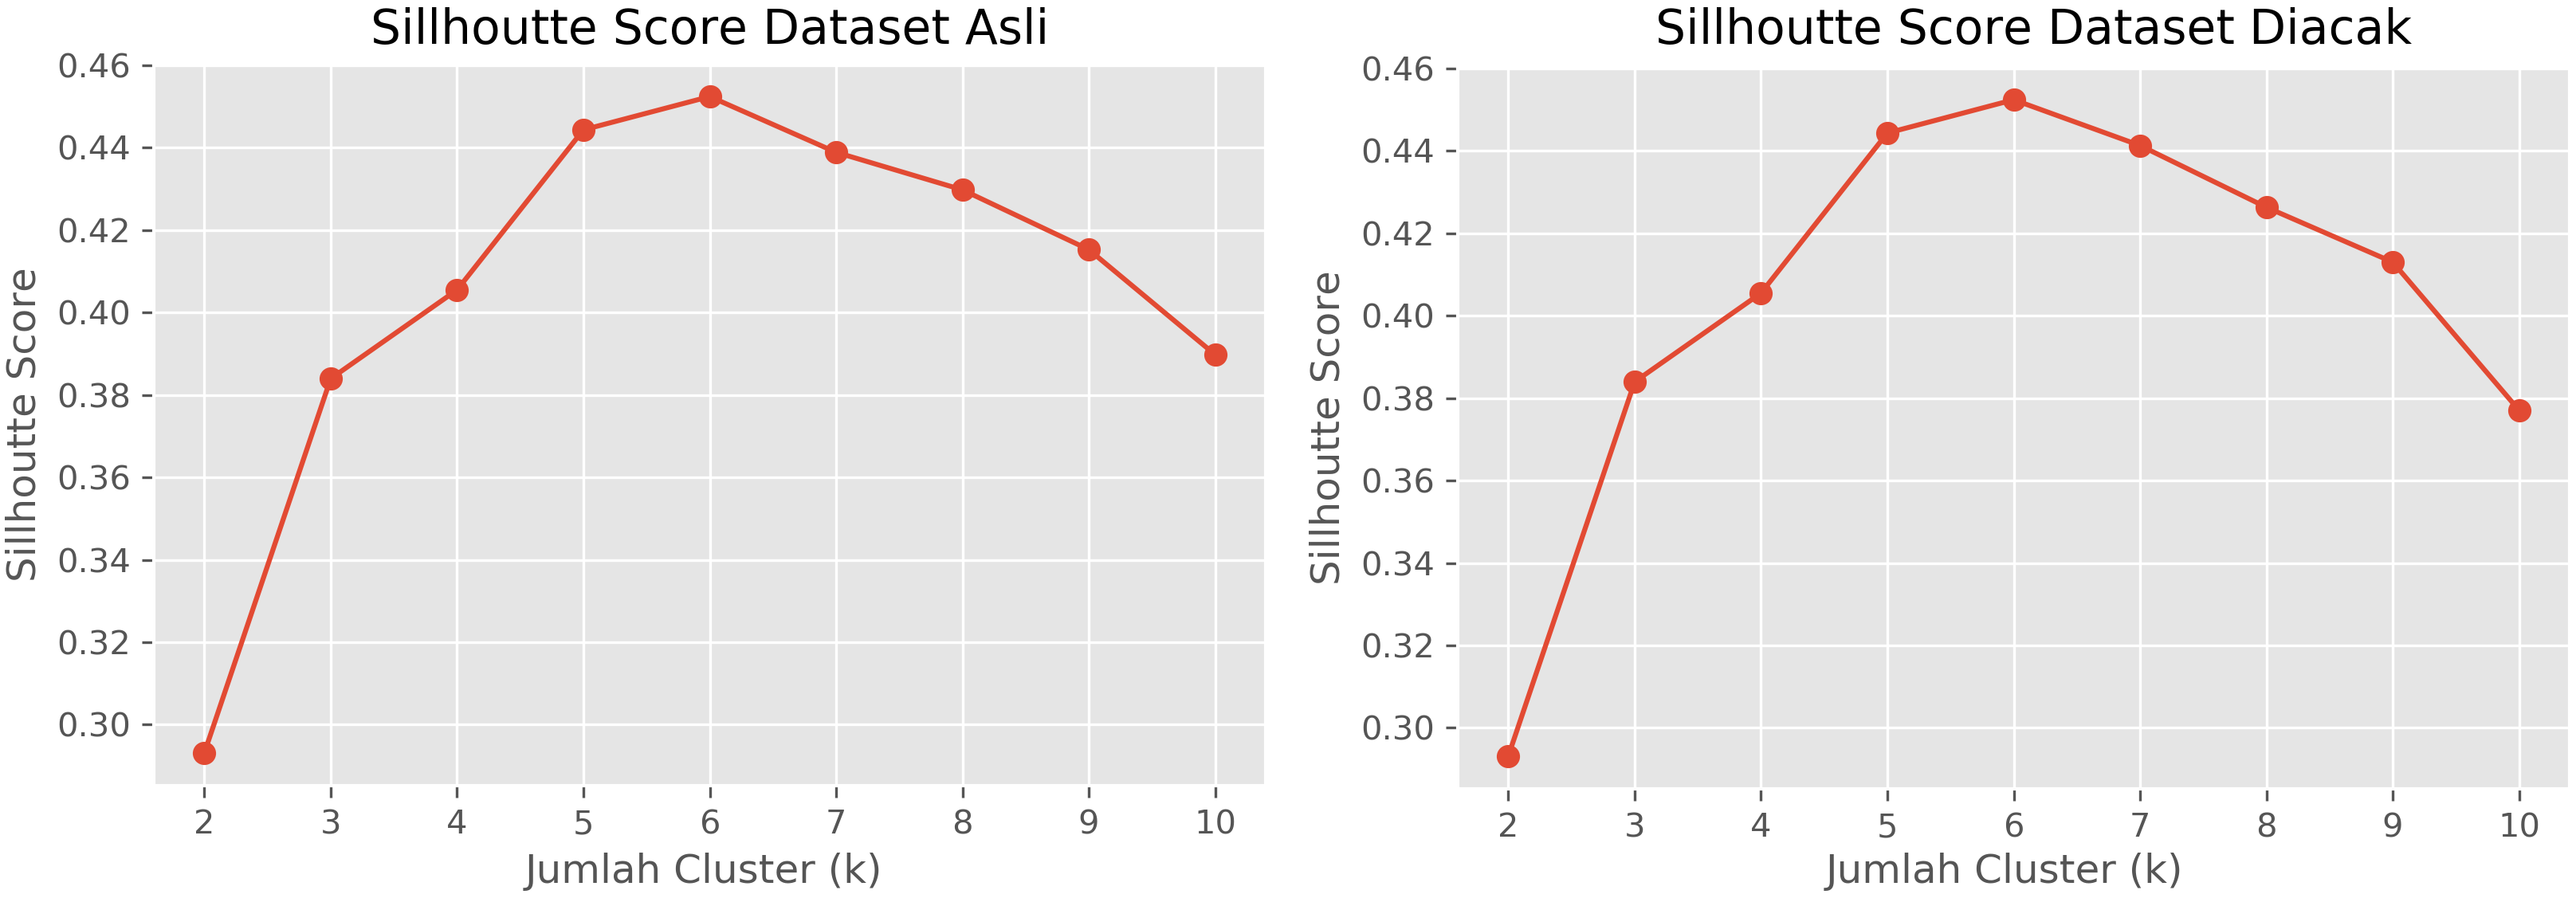
\includegraphics[scale=0.185]{siluet_mall_customers}
		\caption{Grafik \textit{Sillhoutte Score} model \textit{clustering} pada dataset \textit{mall\_customers}}
		\label{fig:siluet_mall_customers}
	\end{figure}
	
	\noindent\begin{minipage}{.44\textwidth}
	\begin{lstlisting}[caption=Sillhoutte Score Dataset Asli,frame=tlrb, label=mall_customers_siluet_asli]{Name}
Sillhoutte Score setiap K
pada dataset asli: 
2: 0.293166070535953
3: 0.3839349967742105
4: 0.40546302077733304
5: 0.44504314844253573
6: 0.4523443947724053
7: 0.43978902692261157
8: 0.42790288922594905
9: 0.4137641526186506
10: 0.3750147687842441
	\end{lstlisting}
	\end{minipage}\hfill
	\begin{minipage}{.44\textwidth}
	\begin{lstlisting}[caption=Sillhoutte Score Dataset Randomisasi,frame=tlrb, label=mall_customers_siluet_randomisasi]{Name}
Sillhoutte Score setiap K
pada dataset randomisasi: 
2: 0.29316607053507854
3: 0.383934996807901
4: 0.40546302082487856
5: 0.44428597567883826
6: 0.4523443947780976
7: 0.44128075766857394
8: 0.42815090435529995
9: 0.3861502477348431
10: 0.3897532214988177
	\end{lstlisting}
	\end{minipage}

	\item Teknik penambangan data \textit{K-means} diterapkan menggunakan empat buah fitur yang ada untuk menguji apakah dataset asli dan dataset yang telah dirandomisasi menghasilkan kluster dan bentuk yang sama dengan sudut yang berbeda saat divisualisasikan. Pengujian tersebut didasarkan pada sifat teknik \textit{Random Rotation Perturbation} yang menjamin jarak Euclidean setiap titik tidak berubah sama sekali tetapi merotasi seluruh titik yang ada pada bidang Euclidean. Akurasi akan dihitung dengan jumlah tetangga (nilai \textit{k}) dari 1 sampai 20. Visualisasi \textit{cluster} pada dataset asli dan dataset yang telah dirandomisasi masing-masing dapat dilihat pada Gambar~\ref{fig:kmeans_mall_asli} dan Gambar~\ref{fig:kmeans_mall_rotated}. Implementasi kode teknik penambangan data ini diterapkan dengan bahasa pemograman Python dan dibantu oleh \textit{library} Scikit-learn. Visualisasi model \textit{clustering} dengan nilai \textit{k} sebesar 6 pada dataset \textit{mall\_customers} asli dan yang telah dirandomisasi dapat dilihat pada Gambar~\ref{fig:kmeans_mall_asli} dan Gambar~\ref{fig:kmeans_mall_rotated}. 

	\begin{figure}
		\centering
		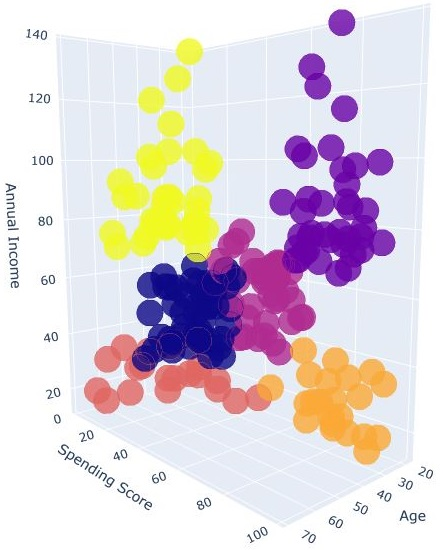
\includegraphics[scale=1]{kmeans_mall_asli}
		\caption{Visualisasi \textit{cluster} pada dataset yang asli}
		\label{fig:kmeans_mall_asli}
	\end{figure}
	
	\begin{figure}
		\centering
		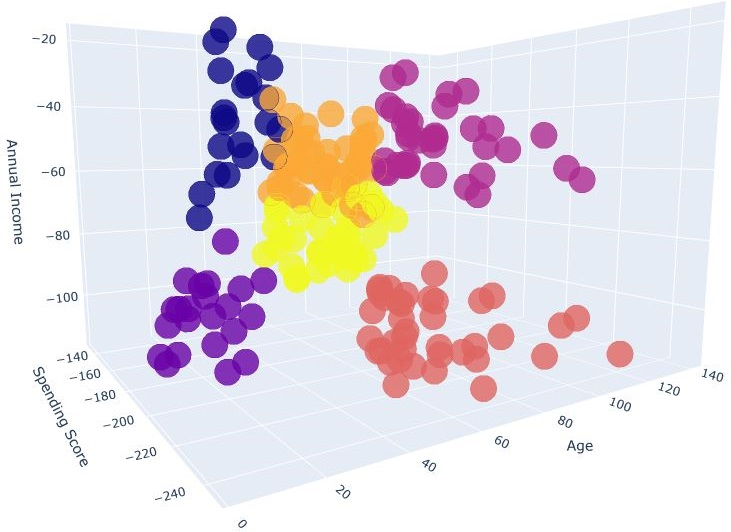
\includegraphics[scale=0.7]{kmeans_mall_rotated}
		\caption{Visualisasi \textit{cluster} pada dataset yang telah dirotasi}
		\label{fig:kmeans_mall_rotated}
	\end{figure}

	Dapat dilihat pada kedua visualisasi tersebut mempunyai jumlah \textit{cluster} yang sama dan terlihat dari lokasi titik-titik yang ada jika dibandingkan terlihat seperti dirotasi searah jarum jam dan bentuknya masih terlihat sama. Apabila dihitung kemiripan \textit{cluster} tersebut dengan metode \textit{Adjusted Rand Index} maka kedua hasil \textit{clustering} tersebut mempunyai nilai 1.0 yang berarti titik-titik yang ada pada setiap \textit{cluster} pada kedua model persis adanya.
	
	\item Waktu eksekusi yang dibutuhkan untuk melatih model \textit{clustering} dengan algoritma \textit{K-means} adalah 0.02995157241821289 detik pada dataset yang asli dan 0.032910823822021484 detik pada dataset yang telah dirandomisasi, hal ini menunjukkan bahwa teknik \textit{Random Rotation Perturbation} tidak memepengaruhi secara signifikan waktu eksekusi untuk melatih model \textit{K-means}.
\end{itemize}

Teknik \textit{Random Rotation Perturbation} terbukti bekerja dengan baik untuk mengacak data sehingga privasi pada data tersebut hilang tetapi data masih dapat digunakan untuk membuat model \textit{clustering} dengan algoritma \textit{K-means} dengan hasil yang memuaskan. 

\subsubsection{\textit{Random Projection Perturbation}}
\label{sec:pengujian-clustering-rpp}

Pengujian teknik \textit{Random Projection Perturbation} untuk penambangan data \textit{clustering} dengan algoritma \textit{K-means} akan dilakukan dengan dataset \textit{mobile\_sensor} yang dapat dilihat 20 baris pertamanya pada Gambar~\ref{fig:mobile_sensor_asli}. Dataset ini dirandomisasi dengan teknik \textit{Random Projection Perturbation} dan hasil randomisasi dapat dilihat pada Gambar~\ref{fig:projected_mobile_sensor}. Dengan kedua dataset tersebut, dilakukan penambangan data terhadap kedua dataset tersebut dan dihasilkan berbagai macam informasi yang dapat dibandingkan. Berikut adalah hasil pengujian dan penjelasannya.

\begin{itemize}
	\item Sebelum melakukan teknik \textit{clustering} dengan algoritma \textit{K-means}, dataset yang memiliki fitur yang sangat banyak tersebut dimensinya harus direduksi terlebih dahulu agar model dapat divisualisasikan dengan mudah. Dataset yang akan di\textit{cluster} akan direduksi dimensinya sampai hanya memiliki 2 dimensi. Reduksi dimensi dilakukan dengan menerapkan teknik \textit{Principal Component Analysis} yang sudah umum digunakan saat penambangan data dan hasilnya relatif baik. Walaupun teknik \textit{Principal Component Analysis} membuat visualisasi mudah untuk dilakukan tetapi ada kekurangannya yaitu sebagian informasi pada dataset akan hilang dan hal ini mempengaruhi hasil \textit{clustering} sehingga \textit{cluster} yang ada akan bersifat lebih umum, tidak spesifik. 
	
	Dalam menguji teknik \textit{Random Projection Perturbation}, dataset yang tidak diterapkan teknik tersebut langsung direduksi dimensinya dengan metode \textit{Principal Component Analysis} dan dataset yang akan dirandomisasi, akan terlebih dahulu diterapkan teknik \textit{Random Projection Perturbation} baru direduksi dimensinya menjadi 2 dimensi dengan metode \textit{Principal Component Analysis}. Visualisasi hasil metode \textit{Principal Component Analysis} dataset yang asli dan yang telah dirandomisasi dapat dilihat pada Gambar~\ref{fig:scatter_mobile_sensor}.

	\begin{figure}
		\centering
		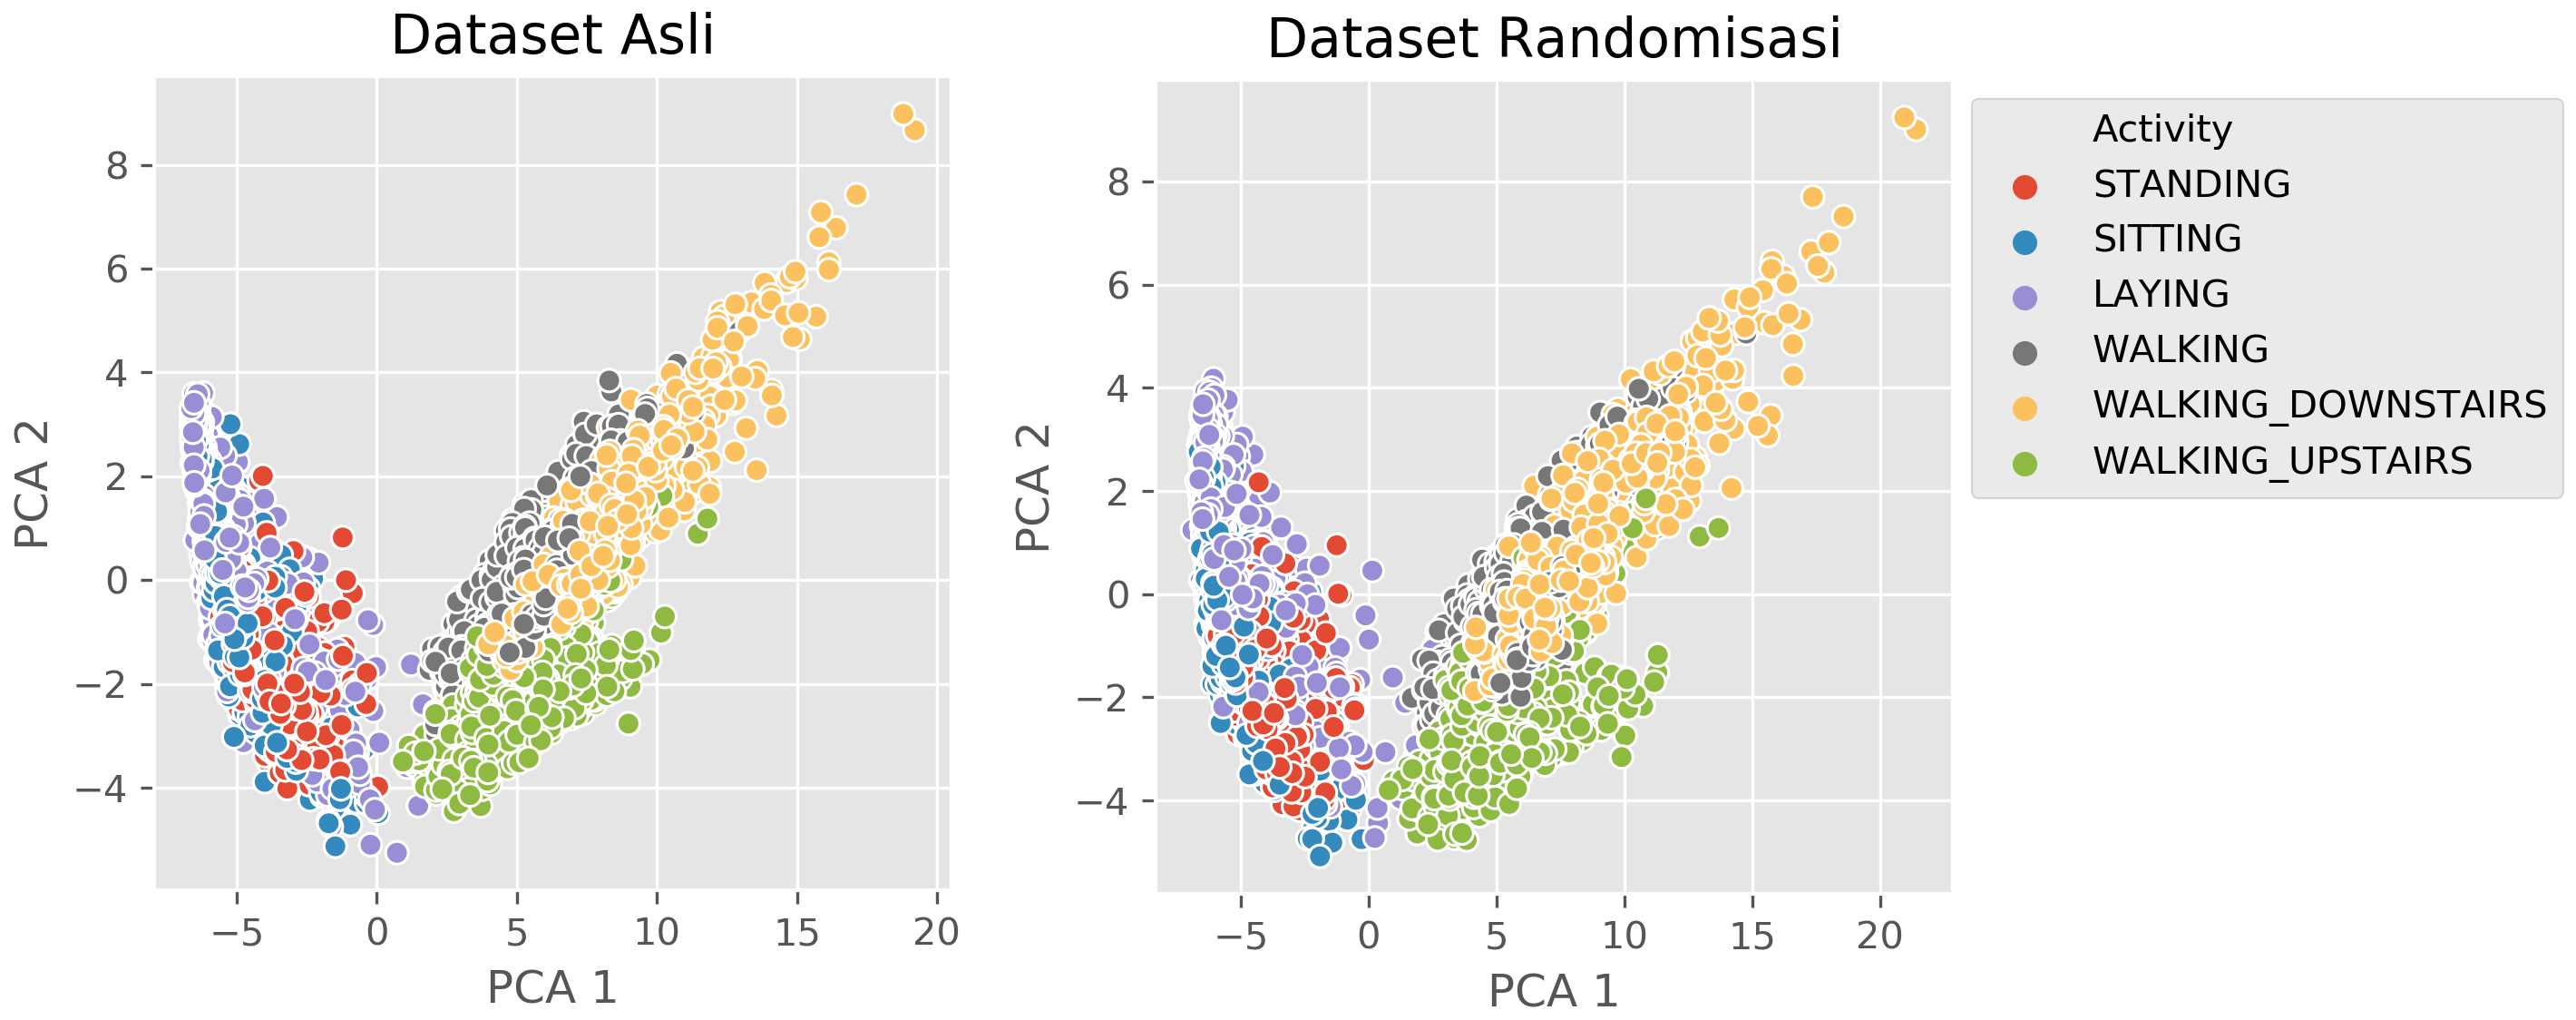
\includegraphics[scale=0.2]{scatter_mobile_sensor}
		\caption{\textit{Scatter plot} dataset \textit{mobile\_sensor} yang telah direduksi dimensinya menjadi 2 dimensi dengan metode \textit{Principal Component Analysis}}
		\label{fig:scatter_mobile_sensor}
	\end{figure}
	\item Pada Gambar~\ref{fig:elbow_mobile_sensor} terdapat grafik \textit{SSE} untuk menggunakan metode Elbow pada dataset asli dan dataset yang telah dirandomisasi. Pada grafik ini tidak terlalu terlihat nilai yang terbaik untuk menjadi nilai \textit{k} yang dipakai pada dataset asli maupun dataset randomisasi. Walaupun seperti itu, pada kedua dataset tersebut grafik \textit{SSE}-nya terlihat sangat mirip dikarenakan teknik \textit{Random Projection Perturbation} menjaga jarak Euclidean dengan baik dan terkontrol. Dalam menentukan nilai \textit{k} yang terbaik untuk dipakai membuat model, \textit{Sillhoutte Score} dapat digunakan untuk metode alternatif untuk menentukan nilai \textit{k} yang terbaik.

	\begin{figure}
		\centering
		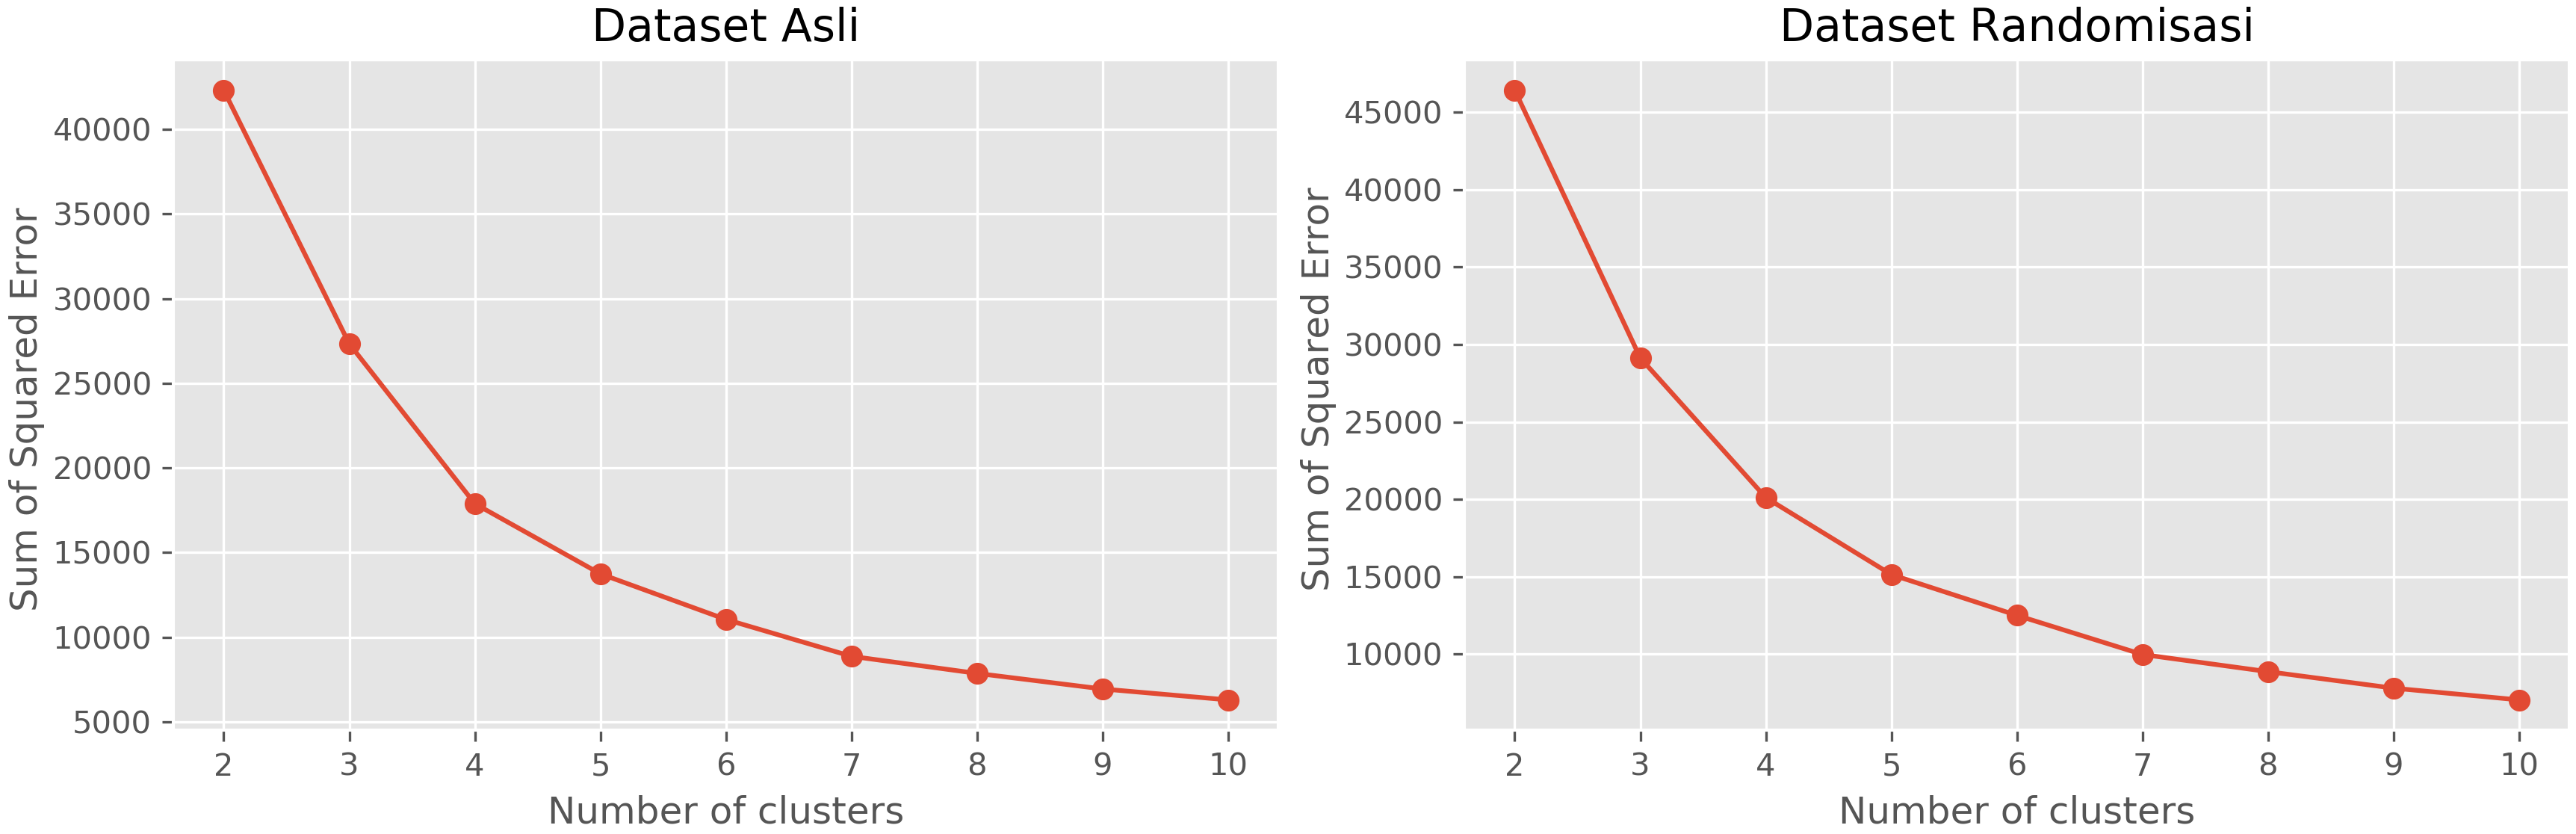
\includegraphics[scale=0.18]{elbow_mobile_sensor}
		\caption{Grafik \textit{SSE} untuk menggunakan metode Elbow untuk mencari nilai \textit{k} terbaik}
		\label{fig:elbow_mobile_sensor}
	\end{figure}
	\item Pada Gambar~\ref{fig:siluet_mobile_sensor} terdapat grafik \textit{Sillhoutte Score} dari dataset \textit{mobile\_sensor} yang asli dan yang telah dirandomisasi. Dapat terlihat kedua grafik \textit{Sillhoutte Score} terlihat sangat mirip dan dapat dilihat nilai-nilai pada setiap \textit{k} tersebut di Listing~\ref{mobile_sensor_siluet_asli} dan Listing~\ref{mobile_sensor_siluet_randomisasi} ada sedikit perbedaan yang tidak terlalu signifikan. Hal ini dikarenakan oleh jarak Euclidean pada dataset asli dan yang telah dirandomisasi sedikit berbeda sehingga mempengaruhi sedikit pada hasil algoritma \textit{Sillhoutte Score}. Dapat terlihat \textit{Sillhoutte Score} pada nilai \textit{k} sebesar 2 adalah nilai paling besar yaitu 0.7568010158989575 pada dataset asli dan 0.7581796759180272 pada dataset yang telah dirandomisasi. Hal ini menunjukkan teknik \textit{Random Projection Perturbation} tidak mempengaruhi secara signifikan nilai \textit{Sillhoutte Score} pada setiap \textit{k}.

	\begin{figure}
		\centering
		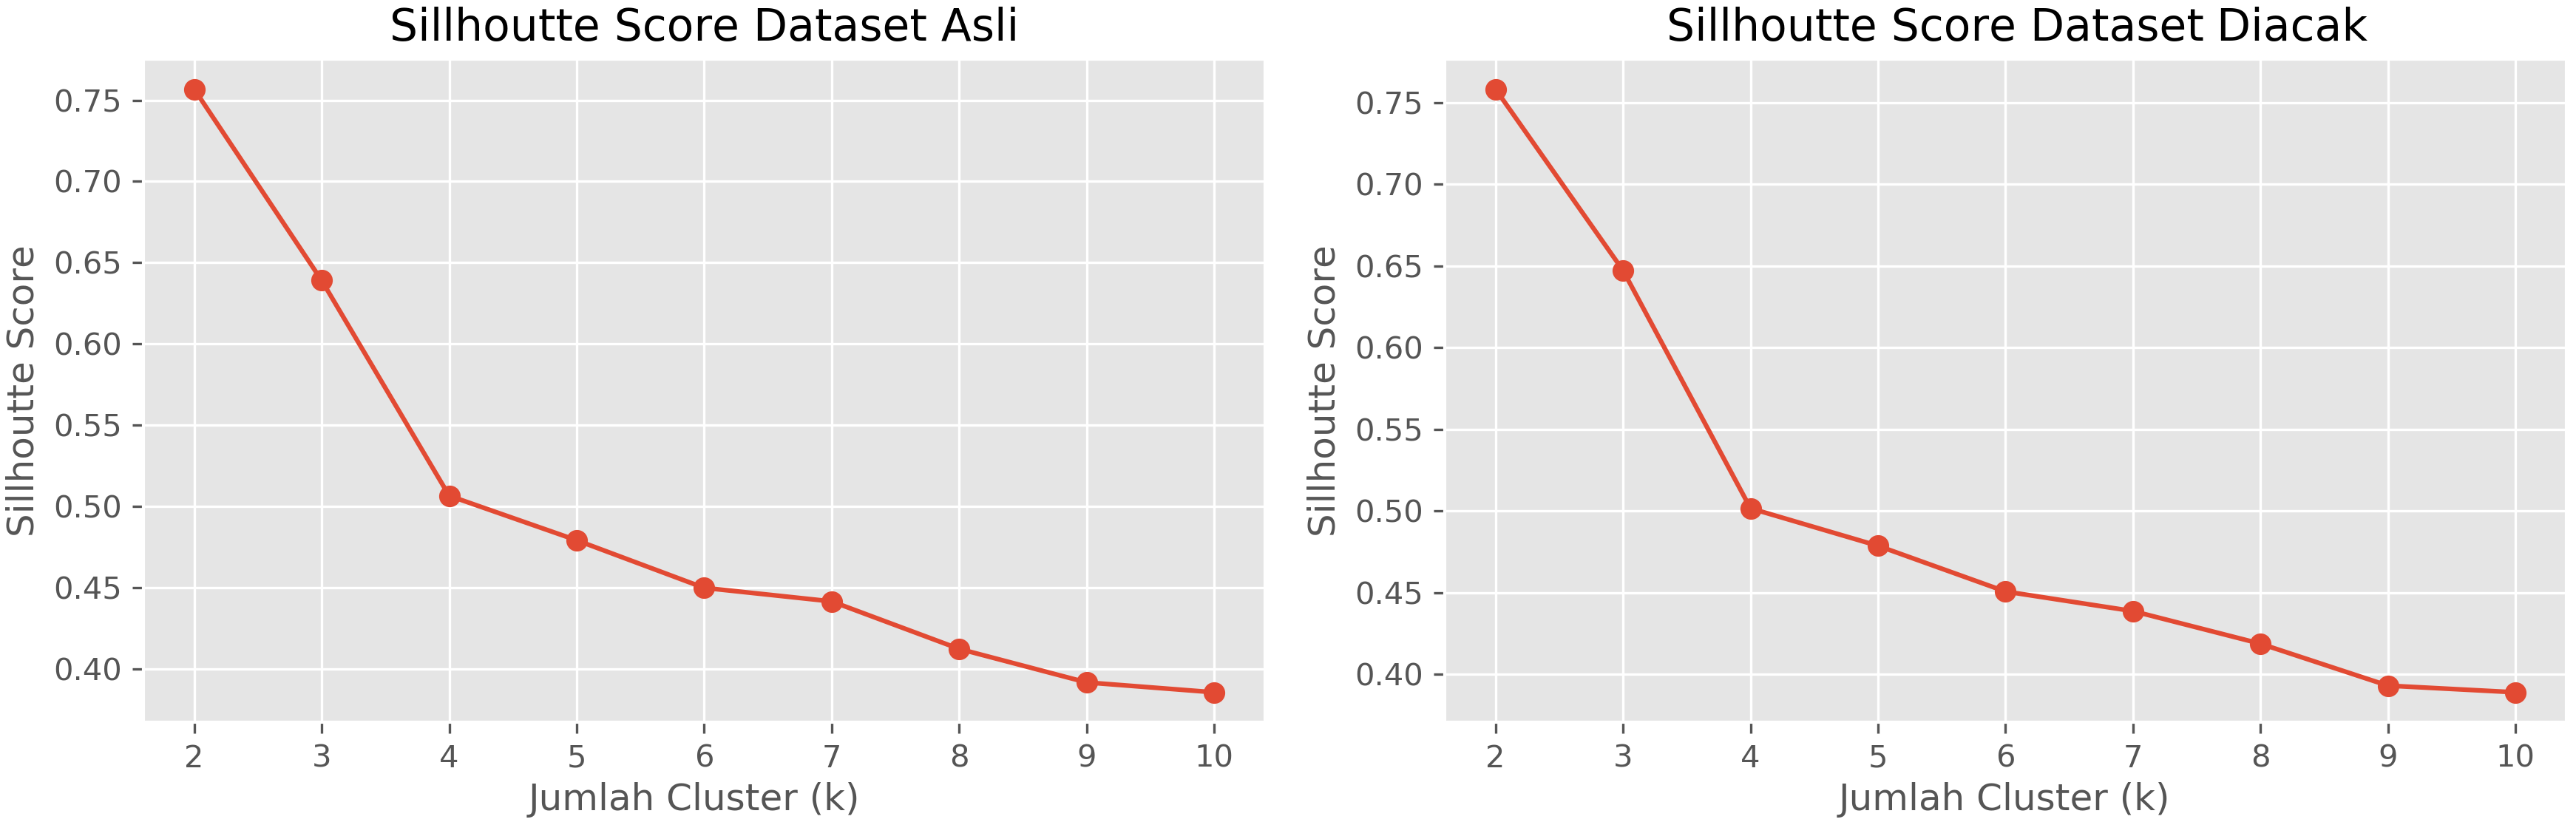
\includegraphics[scale=0.175]{siluet_mobile_sensor}
		\caption{Grafik \textit{Sillhoutte Score} model \textit{clustering} pada dataset \textit{mobile\_sensor}}
		\label{fig:siluet_mobile_sensor}
	\end{figure}
	
	\noindent\begin{minipage}{.44\textwidth}
	\begin{lstlisting}[caption=Sillhoutte Score Dataset Asli,frame=tlrb, label=mobile_sensor_siluet_asli]{Name}
Sillhoutte Score setiap K
pada dataset asli: 
2: 0.7568010158989575
3: 0.6390101777235029
4: 0.506497255331499
5: 0.4790910470659918
6: 0.4497981866661921
7: 0.4414685328088866
8: 0.4122363491089296
9: 0.39158160384319435
10: 0.3854996654126945
	\end{lstlisting}
	\end{minipage}\hfill
	\begin{minipage}{.44\textwidth}
	\begin{lstlisting}[caption=Sillhoutte Score Dataset Randomisasi,frame=tlrb, label=mobile_sensor_siluet_randomisasi]{Name}
Sillhoutte Score setiap K
pada dataset randomisasi: 
2: 0.7581796759180272
3: 0.6472419899391577
4: 0.5015650888399312
5: 0.47862510668209096
6: 0.45064475921629954
7: 0.43865532313764366
8: 0.4186927518384631
9: 0.3930205669353965
10: 0.3889412224520463
	\end{lstlisting}
	\end{minipage}
	\item Teknik penambangan data \textit{K-means} diterapkan menggunakan dua buah fitur yang ada hasil dari teknik \textit{Principal Component Analysis} untuk menguji apakah dataset asli dan dataset yang telah dirandomisasi menghasilkan \textit{cluster} yang hampir sama. Pengujian tersebut didasarkan pada sifat teknik \textit{Random Projection Perturbation} yang menjamin jarak Euclidean terjaga dengan besar \textit{error} yang ditentukan pengguna. Model \textit{K-means} akan dibuat dengan nilai \textit{k} yang terbaik dihitung menggunakan metode Elbow dan nilai \textit{k} yang memiliki \textit{Sillhoutte Score} tertinggi. Implementasi kode teknik penambangan data ini diterapkan dengan bahasa pemograman Python dan dibantu oleh \textit{library} Scikit-learn. 

	Visualisasi model \textit{clustering} dengan nilai \textit{k} sebesar 2 pada dataset \textit{mobile\_sensor} asli dan yang telah dirandomisasi dapat dilihat pada Gambar~\ref{fig:kmeans_mobile_sensor_asli} dan Gambar~\ref{fig:kmeans_mobile_sensor_randomisasi}. Dapat dilihat pada kedua visualisasi tersebut mempunyai jumlah \textit{cluster} yang sama yaitu 2 \textit{cluster} dan terlihat dari lokasi titik-titik yang ada jika dibandingkan ada sedikit perbedaan tetapi tidak terlalu signifikan. Hasil \textit{clustering} menyatakan bahwa ada dua buah \textit{cluster} yaitu kelompok orang-orang yang diam dan kelompok orang-orang yang bergerak, hasil \textit{clustering} ini tidak secara spesifik menentukan aktivitas setiap orang karena informasi tersebut sudah hilang oleh teknik yang digunakan sebelumnya, \textit{Principal Component Analysis}. 
	
	\begin{figure}
		\centering
		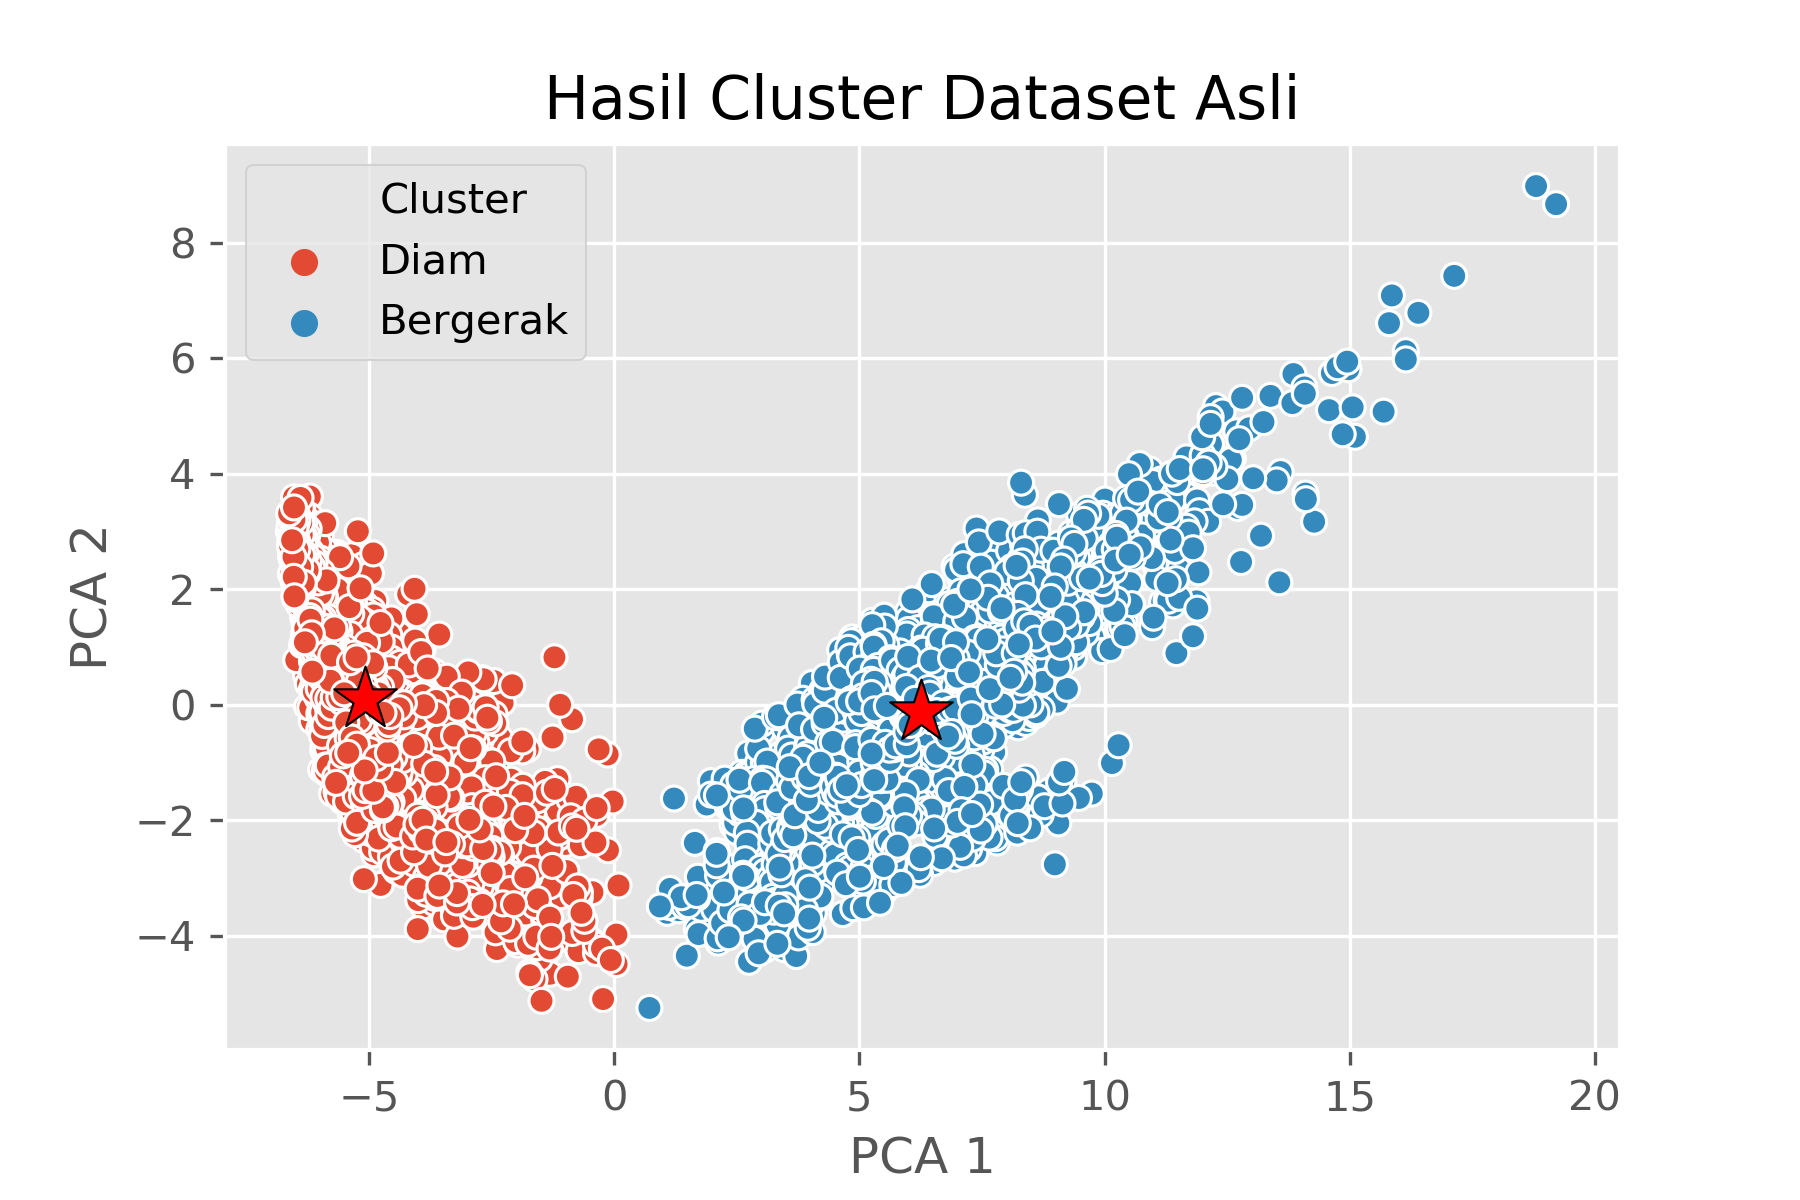
\includegraphics[scale=1]{kmeans_mobile_sensor_asli}
		\caption{Visualisasi \textit{cluster} pada dataset yang asli}
		\label{fig:kmeans_mobile_sensor_asli}
	\end{figure}
	
	\begin{figure}
		\centering
		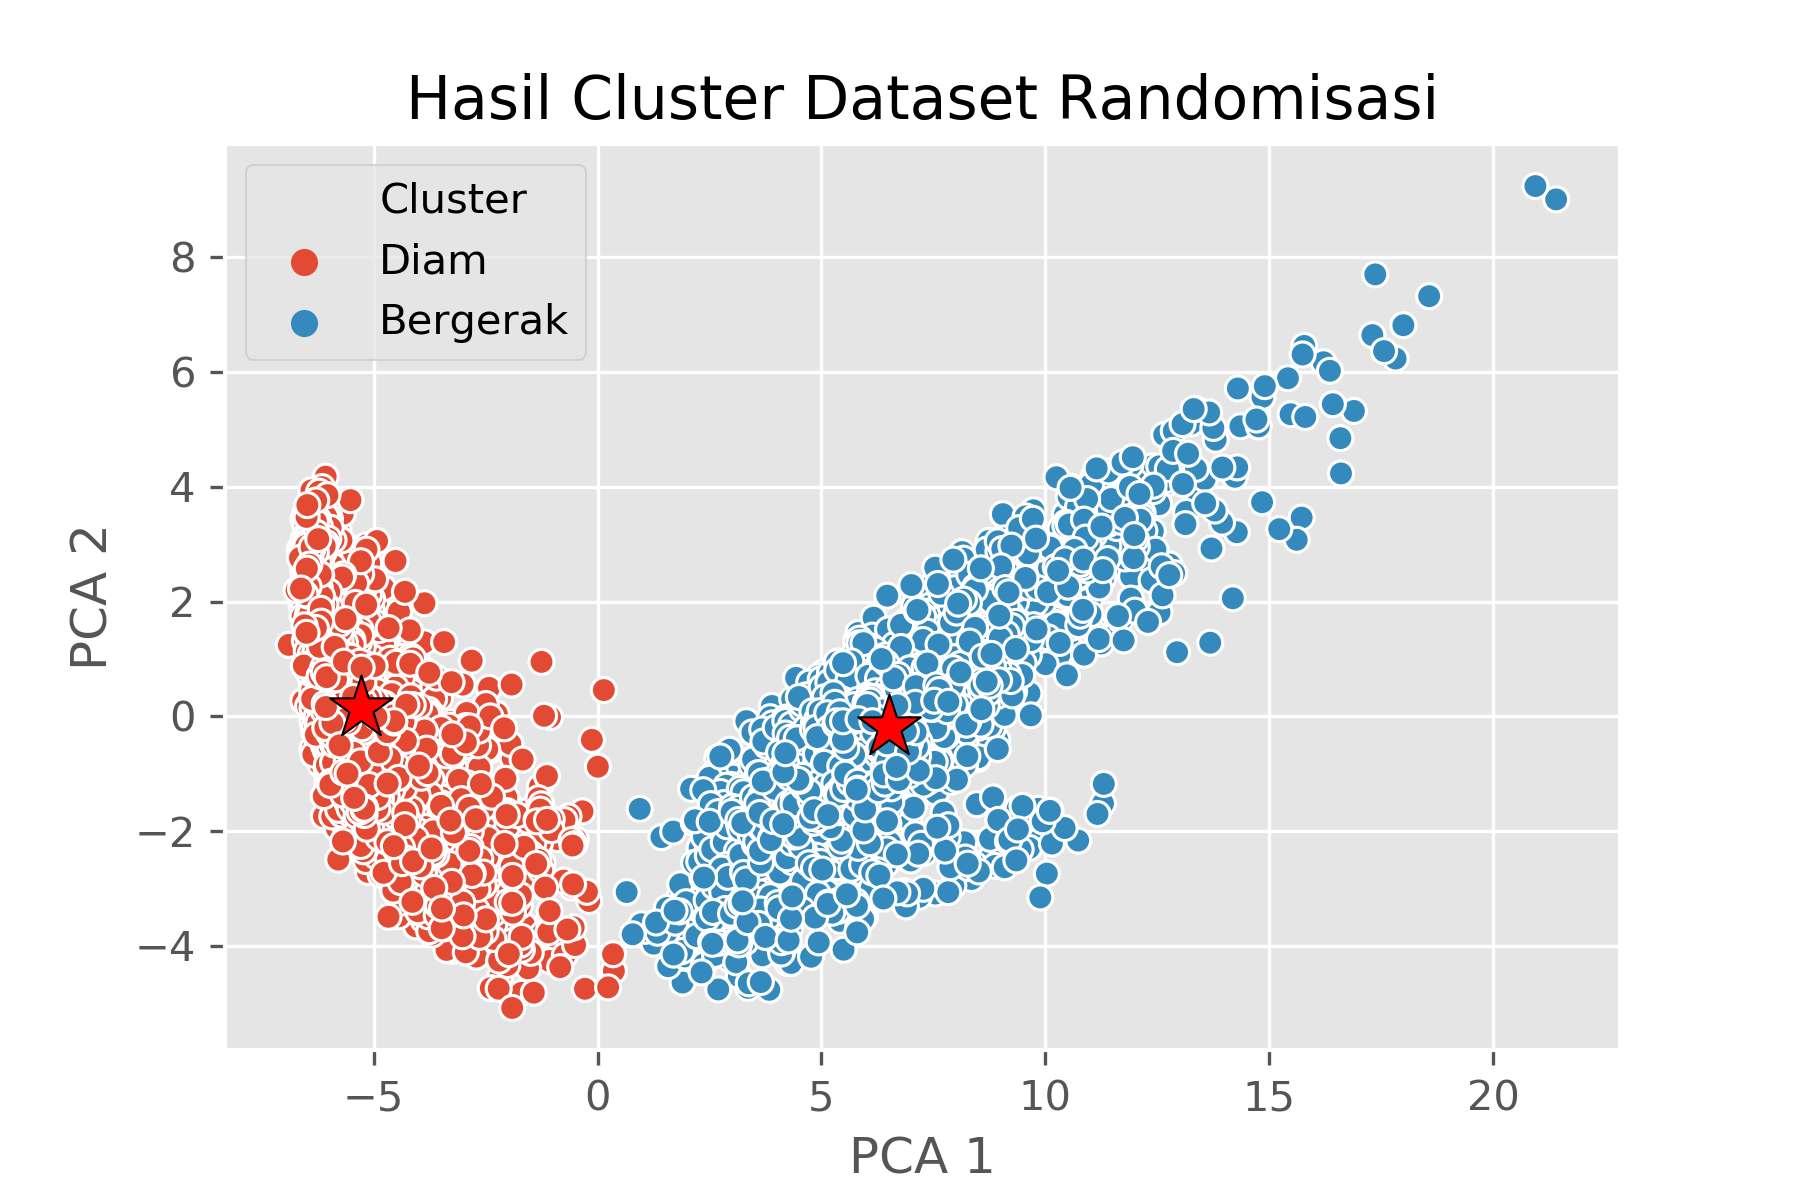
\includegraphics[scale=1]{kmeans_mobile_sensor_randomisasi}
		\caption{Visualisasi \textit{cluster} pada dataset yang telah diproyeksi}
		\label{fig:kmeans_mobile_sensor_randomisasi}
	\end{figure}
	
	\item Apabila dihitung kemiripan \textit{cluster} tersebut dengan metode \textit{Adjusted Rand Index} maka kedua hasil \textit{clustering} tersebut mempunyai nilai 0.9994558701020273 yang berarti titik-titik yang ada pada setiap \textit{cluster} pada kedua model sangat mirip sekali. Hal ini dikarenakan jarak Euclidean kedua buah dataset tidak rusak secara signifikan dan \textit{error}nya terkendali sesuai yang pengguna inginkan.
	\item Waktu eksekusi yang dibutuhkan untuk melatih model \textit{K-means} dengan nilai \textit{k} sebesar 2 adalah sebesar 0.031239032745361328 detik pada dataset asli dan 0.031217575073242188 detik pada dataset yang telah dirandomisasi. Jika dibandingkan, kedua dataset memiliki waktu eksekusi yang hampir sama, hal ini dikarenakan kedua dataset tersebut diterapkan terlebih dahulu teknik \textit{Principal Component Analysis} sehingga kedua dataset memiliki ukuran yang sama. Perbedaan pada kedua dataset dapat terlihat pada waktu eksekusi teknik  \textit{Principal Component Analysis} pada kedua dataset yang mana masing-masing sebesar 0.1405951976776123 detik dan 0.1093449592590332 detik. Oleh karena itu, teknik \textit{Random Projection Perturbation} mempengaruhi waktu eksekusi karena ukuran dataset berkurang sehingga waktu eksekusinya juga berkurang.
\end{itemize}

Teknik \textit{Random Projection Perturbation} terbukti bekerja dengan baik untuk mengacak data sehingga privasi pada data tersebut hilang tetapi data masih dapat digunakan untuk membuat model \textit{clustering} dengan algoritma \textit{K-means} dan menggunakan teknik \textit{Principal Component Analysis} dengan hasil yang memuaskan.
